\newcommand{\typeOfWork}{Master Thesis}
\newcommand{\titleToObtain}{Master of Science in Engineering}
\newcommand{\studyProgram}{Master Program Cloud Computing Engineering}
\newcommand{\yourNameInclTitle}{Thomas Stadler, BSc}
\newcommand{\yourMatNumber}{12345678}
\newcommand{\supervisorNameInclTitle}{Akademische(r) Grad(e)  Vorname Zuname}
\newcommand{\departmentName}{Department Informationstechnologie und Informationsmanagement}
\newcommand{\yourThesisTitle}{Energieeffizienz-orientiertes adaptives Scheduling in heterogenen Clustern}
\newcommand{\thesisDate}{March \ordinalnum{17} 2021}
\newcommand{\universityCityCountry}{FH-Burgenland, Eisenstadt, Österreich}
\newcommand{\thesisBookLiteratureLabel}{References}

% choose a language
%\newcommand{\toObtainLabel}{for obtaining the academic degree}
\newcommand{\submittedByLabel}{Submitted by:}
\newcommand{\matNumberLabel}{Matriculation number:}
\newcommand{\dateLabel}{Date:}
\newcommand{\advisorLabel}{Supervised by:}
\newcommand{\toObtainLabel}{zur Erlangung des akademischen Grades}
\newcommand{\submittedByLabel}{Eingereicht von:}
\newcommand{\matNumberLabel}{Personenkennzeichen:}
\newcommand{\dateLabel}{Datum:}
\newcommand{\advisorLabel}{Betreut von:}

% choose a format
\input{00_preamble/thesis-book}

% if not used with overleaf add data input here
%\input{01_data/yourData}
\hypersetup{
    pdftitle={\yourThesisTitle},
    pdfsubject={\typeOfWork},
    pdfauthor={\yourNameInclTitle},
    breaklinks, % permits line breaks for long links
    bookmarksnumbered,        % ... and include section numbers
    linktocpage,        % "make page number, not text, be link on TOC ..."
    colorlinks,            % yes ...
    linkcolor=black,        % normal internal links;
    anchorcolor=black,   
    citecolor=black,
    urlcolor=blue,        % quite common
    pdfstartview={Fit},        % "Fit" fits the page to the window
    pdfpagemode=UseOutlines,    % open bookmarks in Acrobat
    plainpages=false      % avoids duplicate page number problem
}

\begin{document}
\pagestyle{empty}
\pagenumbering{gobble}


\begin{flushleft}
    \LARGE{\yourThesisTitle}
\end{flushleft}
\subsectionfont{\fontsize{13}{16}\normalfont}
\titlespacing\subsection{0pt}{0ex}{0ex}
\subsection*{\yourNameInclTitle}
\vspace{-0.5em}
\noindent{\textit{\universityCityCountry}}

% define header appearance
\titleformat{\chapter}{\normalfont\large}{\thechapter}{20pt}{\normalfont\large\MakeUppercase}
\chapterfont{\fontsize{13}{16}\normalfont\MakeUppercase}
\titlespacing\chapter{0pt}{2ex}{2ex}
\sectionfont{\fontsize{13}{16}\normalfont}
\titlespacing\section{0pt}{0ex}{0ex}
\subsectionfont{\fontsize{13}{16}\normalfont}
\titlespacing\subsection{0pt}{0ex}{0ex}
\subsubsectionfont{\fontsize{13}{16}\normalfont}
\titlespacing\subsection{0pt}{0ex}{0ex}
% numbering subsubsections
\setcounter{secnumdepth}{5}

% do not start chapter on new page
\makeatletter
\patchcmd{\chapter}{\clearpage}{\leavevmode\flushleft}{}{}
\makeatother

\vspace{5em}
\begin{abstract}
    \input{A_FrontMatter/abstract-plain-de}
\end{abstract}
\vspace{2em}
%\input{B_Chapters/01_Introduction}
%\input{B_Chapters/02_Fundamentals}
%\input{B_Chapters/03_Methodology}
%\input{B_Chapters/04_Empirical_work}
%\input{B_Chapters/05_Discussion}
%\input{B_Chapters/06_Synopsis}
\input{B_Chapters/TB_Einleitung_und_Problemhintergrund}

\titleformat{\chapter}{\normalfont\Large}{\thechapter}{20pt}{\normalfont\Large}
\printbibliography[title=\thesisBookLiteratureLabel]
\end{document}


% if not used with overleaf add data input here
%% if not using overleaf - data is needed separately
\newcommand{\typeOfWork}{Master Thesis}
\newcommand{\titleToObtain}{Master of Science in Engineering}
\newcommand{\studyProgram}{Master Program Cloud Computing Engineering}
\newcommand{\yourNameInclTitle}{Akademische(r) Grad(e)  Vorname Zuname}
\newcommand{\yourMatNumber}{12345678}
\newcommand{\supervisorNameInclTitle}{Akademische(r) Grad(e)  Vorname Zuname}
\newcommand{\departmentName}{Department Informationstechnologie und Informationsmanagement}
\newcommand{\yourThesisTitle}{Please enter your Thesis Title here, up to 70 characters. If necessary, adapt spaces in FHBgld\_Thesis.}
\newcommand{\thesisDate}{March \ordinalnum{17} 2021}
\newcommand{\universityCityCountry}{FH-Burgenland, Eisenstadt, Österreich}
\newcommand{\thesisBookLiteratureLabel}{Literaturverzeichnis}
\hypersetup{
    pdftitle={\yourThesisTitle},
    pdfsubject={\typeOfWork},
    pdfauthor={\yourNameInclTitle},
    breaklinks, % permits line breaks for long links
    bookmarksnumbered,        % ... and include section numbers
    linktocpage,        % "make page number, not text, be link on TOC ..."
    colorlinks,            % yes ...
    linkcolor=black,        % normal internal links;
    anchorcolor=black,   
    citecolor=black,
    urlcolor=blue,        % quite common
    pdfstartview={Fit},        % "Fit" fits the page to the window
    pdfpagemode=UseOutlines,    % open bookmarks in Acrobat
    plainpages=false      % avoids duplicate page number problem
}

\begin{document}
\pagestyle{empty}
\pagenumbering{gobble}


\begin{flushleft}
    \LARGE{\yourThesisTitle}
\end{flushleft}
\subsectionfont{\fontsize{13}{16}\normalfont}
\titlespacing\subsection{0pt}{0ex}{0ex}
\subsection*{\yourNameInclTitle}
\vspace{-0.5em}
\noindent{\textit{\universityCityCountry}}

% define header appearance
\titleformat{\chapter}{\normalfont\large}{\thechapter}{20pt}{\normalfont\large\MakeUppercase}
\chapterfont{\fontsize{13}{16}\normalfont\MakeUppercase}
\titlespacing\chapter{0pt}{2ex}{2ex}
\sectionfont{\fontsize{13}{16}\normalfont}
\titlespacing\section{0pt}{0ex}{0ex}
\subsectionfont{\fontsize{13}{16}\normalfont}
\titlespacing\subsection{0pt}{0ex}{0ex}
\subsubsectionfont{\fontsize{13}{16}\normalfont}
\titlespacing\subsection{0pt}{0ex}{0ex}
% numbering subsubsections
\setcounter{secnumdepth}{5}

% do not start chapter on new page
\makeatletter
\patchcmd{\chapter}{\clearpage}{\leavevmode\flushleft}{}{}
\makeatother

\vspace{5em}
\begin{abstract}
    % TODO:  abstract!

\noindent
Aus den Prinzipien von DevOps entstand GitOps,
als eine Sammlung von Prinzipien und Best Practices
für die Operation von Softwaresystemen. Im Zentrum
bzw. der Quelle - als einzig wahre Quelle (Single Source of Truth) -
steht dabei das Git-Repository bzw. ein Revisions-Kontrollsystem.
Der Zustand des zu verwaltenden Systems wird
vollständig deklarativ als Code definiert. Ein GitOps-Controller
kümmert sich um den kontinuierlichen Abgleich zwischen dem
definierten Ziel-Zustand und dem tatsächlichen Systemzustand.
Die Promotion neuer Software-Releases zwischen mehreren Umgebungen
zeigt sich als derzeit offenes Problem.
Es fehlen einheitliche Standardpraktiken, sowie nötige Tools in der Open-Source-Community.
Diese Arbeit hat als Ziel,
die Promotion von Releases in GitOps-Umgebungen
zu addressieren.
Es sollen abstrakte Modelle von Deployment-Umgebungen
sowie Promotion-Workflows definiert werden.
Aufbauend auf den zuvor definierten Modellen soll eine
standardisierte Lösung zur Promotion von Releases
nach den GitOps-Prinzipien implementiert,
und den bestehenden Lösungen gegenübergestellt werden.

%Der Leser der Kurzfassung soll verstehen, welche Problemstellung / Fragestellung durch die vorliegende Arbeit bearbeitet wird und welche Erkenntnisse und Ergebnisse vorliegen.



\end{abstract}
\vspace{2em}
%
\chapter{Introduction}

TODO

\section{Problem Statement}

% 1. Absatz: Beschreibe uns das Forschungsfeld in dem du dich befindest (DevOps / GitOps)

%\noindent
Increasingly more organizations are adopting 
a DevOps culture to develop new applications and services at high velocity. 
After all, a culture that encourages shared responsibility, transparency and rapid feedback, 
helps to narrow the gaps between teams and thus accelerate the development process.
In order to
reduce friction between engineering teams who are involved in the software development lifecycle (SDLC),
a new practice called GitOps has emerged.
It allows developers who are already familiar with the revision control system Git,
to easily deploy their applications to target environments in a self-service model.
System administrators and operators can also manage IT infrastructure
purely by interfacing with declarative state definitions stored in Git.
%GitOps is a set of principles for operating and managing software systems.
%These principles are derived from modern software operations, but also have their roots 
%in existing and widely adopted best practices. 
\bigskip

% 2. Absatz: Beschreib uns das Problem bzw. die Challenge in diesem Forschungsfeld (Was ist die Problemstellung, die es zu bearbeiten gilt)

% why is it important to solve the problem?

\noindent
GitOps as a practice for releasing software has many advantages,
but like other solutions, GitOps also has some shortcomings.
One of the unresolved problems is
the process of promoting releases between multiple deployment environments (illustrated in Figure \ref{fig:releasePromotionProcess}).

\begin{figure}[h]
	\centering
	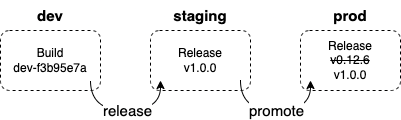
\includegraphics[width=.55\linewidth]{figures/release-promotion.drawio.png}
	\caption{release promotion process.
		%		(\citeauthor{ref}, \citeyear{ref}).
	}
	\label{fig:releasePromotionProcess}	
\end{figure}

\noindent
Current GitOps tools do not provide an integrated solution for this process,
nor do they provide any sort of abstraction for defining environments.
Users currently need to rely on separation of duties
on a file and folder level within the Git repository,
for modeling different environments.
Promotions are often achieved via hard-coded file copy operations,
which is done manually or by a
Continuous Integration (CI)/Continuous Delivery (CD) system.
Due to the nature of Git, a certain flow of promotion can not currently be enforced
(e.g. QA --> Staging --> Production).
Furthermore, for each configuration or templating tool which is used
(e.g. kustomize, helm, jsonnet, etc.),
the modeling of different deployment environments, as well as the
process of promotion, is unique.
This results in the process of promoting releases with GitOps
not being a streamlined task.
Clear guidelines and best practices,
as well as tools which implement them,
are missing in the GitOps ecosystem.
\bigskip

% 3. Absatz: Was schlägst du vor, wie man die Problemstellung bearbeiten könnte? Beschreibe uns deinen Lösugnsvorschlag dieser Arbeit, wie man das Problem bearbeiten könnte

\noindent
%
The given problem could be addressed by
providing standardised models 
for defining deployment environments and promotion processes.
%
An application programming interface (API) extension for Kubernetes
could provide custom resource definitions for these models.
%
This would allow users to define abstract representations of
their environments,
and how they want releases to be promoted between them.
%
Additional logic could be introduced into the promotion process,
like specifying a rule which ensures that new releases must first pass
certain environments or other objectives before being promoted to production.
%
The abstraction would also enable transparent replacement of the
configuration or templating tool,
while keeping the desired state definition intact.
%
Following the principles of GitOps,
an operator would ensure the continuous reconciliation
between the desired and the actual state of the resources.
\bigskip

% 4. Absatz: gib uns einen Ausblick (Paint the Big Picture) wie deine Lösung mit dem großen Ganzen zusammenhängt

\noindent
%
The proposed solution of the problem should
present a possible way of defining environments and promotion processes abstractly,
onto which future work could build upon.
%
Additionally the solution should
provide a protoype of a toolkit,
which could serve as an optional component
in addition to existing tooling within the Cloud Native Computing Foundation (CNCF).
%
Solving the problem of release promotion natively within the GitOps toolkit,
would make the adoption of GitOps more appealing,
especially for organisations, which have the need for many different environments.
%
As a result
this could generally accelerate the widespread use of GitOps
and thus enable more organisations to develop higher quality software.
%








\section{Research Questions}
\label{introduction:research-question}


% TODO: goal of this reasearch is ...
%The goal of this thesis is to
%address the problem of promoting releases between different environments in GitOps.
%\bigskip
%
%\noindent
Large organizations in particular typically have many
non-production and production environments
such as:
Development (Dev),
Quality Assurance (QA),
Staging-US,
Staging-EU,
Production-US,
Production-EU.
Usually new releases are automatically deployed to an environment,
such as QA, 
by a CI/CD system.
Now the task is to promote
new changes, which are brought about by a new release,
into subsequent or other environments.
Current GitOps tools do not have a simple answer to
the question about what is the right approach for the process of promotion.
\bigskip

%\noindent
%In particular, this thesis aims to explore
%existing strategies for the solution of the problem
%with existing tools.
%Furthermore, a prototype of a newly proposed strategy will be developed.
%Subsequently, the prototype will be tested in a laboratory experiment
%and compared to currently existing strategies.
%\bigskip

\noindent
To achieve the goal of the thesis, the following research questions (RQ) were identified:

\begin{itemize}
	\item RQ 1: How can the promotion of releases in GitOps environments be designed?
	\begin{itemize}
		\item RQ 1.1: What possibilities do existing tools offer for the promotion of releases with multiple deployment environments?
		\item RQ 1.2: How can deployment environments, as well as promotion processes be modeled abstractly?
		\item RQ 1.3: How can the abstract models be used to implement a standardized solution for promoting releases?
	\end{itemize}
\end{itemize}

% ensure bullet points do not span over page break on final PDF export






\section{Research Methodology}
\label{introduction:research-methodology}







\section{Thesis Structure}
\label{introduction:thesis-structure}








%Welcome to the \LaTeX{} template prepared for the Computer Science department at the university of applied sciences of Burgenland\footnote{\url{https://www.fh-burgenland.at/en/information-technology/about-the-department/}}. 
%
%Introduction, Problem, Objective, Demarcation, Question, Method, and a description of the overall structure should go into this chapter.


%
%\section{Instruction included in the original FHBgld word processor template}
%\subsection{Problem stating[!]}
%In der Problemstellung erfolgt eine Hinführung zum Thema aus dem globalen
%Zusammenhang heraus betrachtet: Warum es wichtig ist, sich mit dem konkreten
%Thema zu beschäftigen bzw. welche Bedeutung hat dieses Thema zum Beispiel für die
%Wirtschaft, Gesellschaft und Umwelt.
%\subsection{Research question and added value}
%Hier werden die konkrete(n)wissenschaftliche(n) Fragestellung(en) klar angeführt.
%Neben dem inhaltlichen Ziel der Arbeit wird fallweise auch angegeben, wie
%vorgegangen wird, um die Fragestellung zu bearbeiten (z.B. mit einem Online-
%Fragebogen). Auch die Zielgruppe der Arbeit und der für die Zielgruppe angestrebte
%Nutzen kann an dieser Stelle angeführt werden.
%Anmerkung:
%Die Erfahrung zeigt, dass es hilfreich ist, das erste Einleitungskapitel an die Betreuerin
%/ an den Betreuer zu schicken und Feedback dazu zu erhalten.
%Bitte auch darauf achten, dass alle Absatz-Abstände gleich groß sind.
%Jedes Kapitel sollte mit einem Satz beginnen und einem Satz enden und ca. mind. 1⁄2
%A4-Seite umfassen.
%
%\section{Using the \LaTeX{} template}
%
%Everything in the template revolves around the\verb|main.tex| file. Here all the other files are put together to create the thesis.
%There are three different sections to consider: 
%\begin{itemize}
%	\item Front Matter,
%	\item Chapters, and
%	\item Back Matter.
%\end{itemize}
%Each section has a folder where you can put the different parts of your thesis. In the Front Matter section you should put everything that comes before your first chapter of the thesis. Respectively, in the Back Matter section you put everything that comes after your last chapter. And finally all the chapters are put into the Chapters folder. You can put things like abstract, summaries, etc... wherever they suit your thesis. In the end it really only matters how you add them into your \verb|main.tex| file. With the \verb|\input{}| command you can add the parts if they should appear in your thesis, the order within the \verb|main.tex| also determines the order in the final pdf.
%
%\subsection{Title-page}
%The Layout of the Title-page is in the \verb|FHBgld_Thesis.cls|, normally it remains unchanged. You can use all the commands as seen in the \verb|Titlepage.tex|. 
%
%The template and also the titlepage is based on the scrbook class. So if you want to use a different class without changing the title page in the \verb|FHBgld_Thesis.cls|, it is recommended creating the title page separately and then include the compiled pdf file here, using the 
%\verb|\includepdf{<filename>}| from the \verb|pdfpages| package. Alternatively, you may use the word template for the title- page and add it using this package. In that way you can avoid any differences to the original title page template. The word templates can be found here:
%\begin{enumerate}
%	\item \url{https://moodle.fh-burgenland.at/pluginfile.php/34046/mod_folder/content/0/03_Vorlage_zur_Erstellung_wissenschaftlicher_Arbeiten\%20V2.8.docx?forcedownload=1}
%	\item \url{https://moodle.fh-burgenland.at/pluginfile.php/34046/mod_folder/content/0/03_Vorlage_zur_Erstellung_wissenschaftlicher_Arbeiten\%20V2.8\%20eng.docx?forcedownload=1}
%\end{enumerate}
%
%If you use the \verb|includepdf| package make sure that the pdf still has the correct metadata afterwards.
%
%\subsection{Citing}
%As per requirement of the FH Burgenland, the template class is configured for APA\footnote{\url{https://ctan.org/pkg/biblatex-apa?lang=en}} style: \verb|[natbib=true, backend=biber, style=apa, sorting=nty]|. It uses Biblatex and the Biber backend. The location of the bibliography file is defined in the \verb|main.tex|. Citation xamples:
%\begin{itemize}
%	\item \verb|\parencite{bibid}| provides \parencite{lamport94}
%	\item \verb|\parencite[p. 123ff]{bibid}| provides \parencite[p. 123ff]{lamport94}
%	\item \verb|\parencite{lamport94,talbot2013using}| provides \parencite{lamport94,talbot2013using}
%\end{itemize}
%
%\subsection{Temporary packages and settings}
%Some packages and settings are included to make creating your thesis easier, e.g. FixMe.
%Before building your final PDF, those should be removed. Use \verb|grep -r RMF *| in the root folder of the template to find the packages and settings that should be removed.
%
%\section{Creating the pdf}
%To create a proper pdf file of your thesis there are some things to consider
%
%\subsection{PDF build}
%The script \verb|build.sh| is provided to compile the thesis in four steps:
%\begin{enumerate}
%	\item pdflatex main.tex
%	\item biber main
%	\item bib2gls main
%	\item pdflatex main.tex
%\end{enumerate}
%\verb+bib2gls+ is used to prepare the indexes for glossaries and acronyms. Both are edited in \verb|defns.bib|, therefore, Jabref can be used to manage entries. 
%
%In case you already have your definitions in \LaTeX{} format, such as
%\begin{itemize}
%	\item \verb|\newacronym{gcd}{GCD}{Greatest Common Divisor}}|, or
%	\item \verb|\newglossaryentry{latex}{name=latex,description={Is a mark up language specially suited for scientific documents}}|
%\end{itemize}
%use \verb|convertgls2bib defns.tex defns.bib| to convert from \LaTeX{} to Bibtex.
%
%\subsection{Embed all fonts in pdf}
%Please make sure that you embed all fonts in your pdf. Also make sure all the fonts of any figures that were used in the document are embedded. 
%If you don't use any pdf figures, pdfLaTeX should embed all fonts automatically.
%
%\subsubsection{Linux}
%On Linux you can use the command \begin{verbatim}
%	pdffonts my_file.pdf
%\end{verbatim}
%to check if the fonts are embbeded. Check if all the fonts listed have a "yes" in the "emb" column. 
%\begin{verbatim}
%name                                 type              encoding         emb sub uni 
%------------------------------------ ----------------- ---------------- --- --- --- 
%BXJBCJ+NimbusSanL-Bold               Type 1            Custom           yes yes no     
%HEMYJL+NimbusSanL-Regu               Type 1            Custom           yes yes no     
%OOJWDR+SFRM1000                      Type 1            Custom           yes yes no      
%OHLNOC+SFRM0900                      Type 1            Custom           yes yes no   
%...
%\end{verbatim}
%For more information see 
%
%\url{https://www.karlrupp.net/2016/01/embed-all-fonts-in-pdfs-latex-pdflatex/}
%\subsubsection{Windows}
%On Windows using the Adobe Acrobat Reader the fonts can be found at
%\begin{verbatim}
%	File > Properties > Fonts
%\end{verbatim}
%For more information please consult
%\begin{enumerate}
%	\item \url{https://helpx.adobe.com/acrobat/using/pdf-fonts.html}
%	
%	\item \url{https://www.overleaf.com/learn/latex/Questions/My_submission_was_rejected_by_the_journal_because_%22Font_XYZ_is_not_embedded%22._What_can_I_do%3F} 
%	\end{enumerate}
%	
%	%\subsection{Making a PDF/A-1 compatible pdf}
%	\subsection{Making a PDF}
%
%	
%	\subsubsection{validation}
%	To validate the produced PDF, you can either use the Preflight tool included in Adobe Acrobat Pro or a free online version. E.g. \url{https://www.pdf-online.com/osa/validate.aspx}.
%	Please take caution as different validation tools can report different results.
%	
%	\subsubsection{metadata}
%	There may be a section in the beginning of a .tex file where you define metadata.
%	Setting your Name, Title, Subject, Keywords and remove/add Information for example. To find out what fields are possible please check here. \url{http://texdoc.net/texmf-dist/doc/latex/pdfx/pdfx.pdf#subsection.2.3}
%	
%	A file containing the metadata (jobname.xmpdata) is created when compiling. 
%	
%	Watch out, the metadata .xmpdata file is only created one time. So if you need to update it you need to clear the cache of overleaf. Or delete the .xmpdata file. It is then recreated the next time you compile. 
%	
%	\url{https://www.overleaf.com/learn/how-to/Clearing_the_cache}
%	
%	You can check the metadata of your PDF with Acrobat Reader by going to File-> properties. Or alternatively check it with an online tool.
%	
%	\subsubsection{figures}
%	As already mentioned, make sure that all the fonts used in the pictures are included. Furthermore transparency in pictures causes issues, please convert transparent figures into their nontransparent version. 
%	
%	Using Linux the command \verb|pdfimages -list <pdf>| shows the typpe of all images used. The type should always be \verb|image| and not \verb|smask|. Check and convert these images.
%	
%	\subsubsection{color}
%	Additionally, there can be problems if figures use different color spaces. Use the same command as before and check if all images use the same color. 
%	
%	If color is really important in your work it might also be a good idea to use an ICC profile for the color. 
%	For more details about colors check \url{http://texdoc.net/texmf-dist/doc/latex/pdfx/pdfx.pdf#subsection.2.5}
%	
%	It is also possible to convert the pictures automatically using ghostscript. But always check the results manually. 
%	
%	\subsubsection{Other errors}
%	Due to the complexity of Latex files there can be many more errors that are not covered here.
%	
%	The Preflight tool included in Adobe Acrobat Pro also has the ability to fix some errors. For example EOL (End of Line) errors can be fixed with its analyize and fix option. 
%	Please also check if any of the following pages might have a solution to your problem:
%	\begin{enumerate}
%		\item \url{https://www.mathstat.dal.ca/~selinger/pdfa/}
%		\item \url{https://blog.zhaw.ch/icclab/creating-pdfa-documents-for-long-term-archiving/}
%		\item german: \url{http://kulturreste.blogspot.com/2014/06/grrrr-oder-wie-man-mit-latex-vielleicht.html}
%		\item \url{https://support.stmdocs.in/wiki/?title=Generating_PDF/A_compliant_PDFs_from_pdftex}
%		\item \url{http://texdoc.net/texmf-dist/doc/latex/pdfx/pdfx.pdf}
%	\end{enumerate}
%	
%	\subsubsection{Tagged PDF}
%	Currently with Latex it is only possible to create files that are in the PDF/A-1b format. The PDF/A-1a format required the PDF to be tagged which is currently not possible in a satisfactory way.
%	A manual tagging with Adobe Acrobat Pro is possible but not recommended.
%	
%	More information about the current status of tagged pdfs can be found here:
%	\begin{enumerate}
%		\item \url{https://umij.wordpress.com/2016/08/11/the-sad-state-of-pdf-accessibility-of-latex-documents/} 
%		\item \url{https://www.tug.org/TUGboat/tb30-2/tb95moore.pdf}
%	\end{enumerate}
%	
%	\subsection{General Remarks to create the pdf}
%	Highest priority should always be the embedding of all fonts. Further compliance with the PDF/A standards is always desired, but talk to your advisor in any case.
%	
%	Please also check the following resources if you have problems and need assistance
%	
%	\begin{enumerate}
%		\item \url{https://spl29.univie.ac.at/fileadmin/user_upload/s_spl29/Studium/abschluss_master/Infoblatt_Hochschulschriften.pdf} 
%		\item \url{https://e-theses.univie.ac.at/E-Theses_erstellen_von_pdf.pdf}
%	\end{enumerate}
%	
%	\section{Further tips on the template}
%	In the following chapters there are some general tips on the elements of Latex. You can check them out if you think they have useful information for you. Then you delete these chapters and replace them with the real chapters of your thesis.

%\chapter{Theoretical Background} 	% Produces section heading.  Lower-level
\label{theoretical-background}

%Basics such as theory, definitions, relevant theories, related work and state of the art should be included here.

TODO

% TODO: maximal 1.1.1 
% TODO: wenns 1.1 gibt, muss es auch 1.2 geben

\section{General Definitions}
\label{theoretical-background:general-definitions}

The following section includes general definitions of terms on the topic.

\subsection*{Cloud Computing}

\begin{quotation}
\noindent
\enquote*{Cloud computing is a model for enabling ubiquitous, convenient, on-demand network access to a shared
	pool of configurable computing resources (e.g., networks, servers, storage, applications, and services) that
	can be rapidly provisioned and released with minimal management effort or service provider interaction.
	This cloud model is composed of five essential characteristics, three service models, and four deployment
	models.}
\autocite{cloudComputingNistDefinition2011}
\end{quotation}

The characteristics are
\autocite{cloudComputingNistDefinition2011}:

\begin{itemize}
	\item On-demand self-service
	\item Broad network access
	\item Resource pooling
	\item Rapid elasticity
	\item Measured service
\end{itemize}

The service models are
\autocite{cloudComputingNistDefinition2011}:

\begin{itemize}
	\item Software as a Service (SaaS)
	\item Platform as a Service (PaaS)
	\item Infrastructure as a Service (IaaS)
\end{itemize}

The deployment models are
\autocite{cloudComputingNistDefinition2011}:

\begin{itemize}
	\item Private cloud
	\item Community cloud
	\item Public cloud
	\item Hybrid cloud
\end{itemize}

\subsection*{Cloud Native Application}

\begin{quotation}
\noindent
\enquote*{A cloud-native application (CNA) is a distributed, elastic and horizontal scalable system composed of (micro)services which isolates state in a
minimum of stateful components. The application and each self-contained
deployment unit of that application is designed according to cloud-focused
design patterns and operated on a self-service elastic platform.}
\autocite{cloudNativeApplicationDefinition2017}
\end{quotation}

\subsection*{Continuous}
\begin{quotation}
\noindent
\enquote*{"Continuous" is intended to match the industry standard term: reconciliation continues to happen, not that it must be instantaneous.}
\autocite{gitopsGlossary}
\end{quotation}

\subsection*{Declarative Description}
\begin{quotation}
\noindent
\enquote*{A configuration that describes the desired operating state of a system without specifying procedures for how that state will be achieved. This separates configuration (the desired state) from the implementation (commands, API calls, scripts etc.) used to achieve that state.}
\autocite{gitopsGlossary}
\end{quotation}

\subsection*{Desired State}
\begin{quotation}
\noindent
\enquote*{The aggregate of all configuration data that is sufficient to recreate the system so that instances of the system are behaviourally indistinguishable. This configuration data generally does not include persistent application data, eg. database contents, though often does include credentials for accessing that data, or configuration for data recovery tools running on that system.}
\autocite{gitopsGlossary}
\end{quotation}

\subsection*{DevOps}

\citeauthor{devopsDefinition2016} (\citeyear{devopsDefinition2016})
define DevOps as
a development methodology aimed at bridging the gap between
development and operations, emphasizing communication and collaboration,
continuous integration, quality assurance and delivery with automated deployment
utilizing a set of development practices
\autocite{devopsDefinition2016}.

\subsection*{Drift}
\begin{quotation}
\noindent
\enquote*{When a system's actual state has moved or is in the process of moving away from the desired state, this is often referred to as drift.}
\autocite{gitopsGlossary}
\end{quotation}

\subsection*{Environment}

An Environment
- or GitOps Environment -
in the context of this thesis
is defined as a target deployment environment for a given application;
e.g. Development, Testing, or Production.
Most of the time this is a Kubernetes cluster or namespace.

In the context of the proposed Kubernetes Custom Resource Definition
Environment, however it represents a folder/directory in a Git repository,
which points to a deployment environment or cluster/namespace as defined
in the previous paragraph.

\subsection*{Feedback}
\begin{quotation}
	\noindent
	\enquote*{Open GitOps follows control-theory and operates in a closed-loop. In control theory, feedback represents how previous attempts to apply a desired state have affected the actual state. For example if the desired state requires more resources than exist in a system, the software agent may make attempts to add resources, to automatically rollback to a previous version, or to send alerts to human operators.}
	\autocite{gitopsGlossary}
\end{quotation}

\subsection*{GitOps}

This thesis aims at adhering to the definition of the term GitOps,
%for the term GitOps, its principles and the glossary around it.
as specified by the CNCF project OpenGitOps.
The overall goal of OpenGitOps is to establish a clear vendor-neutral,
principle-driven meaning of GitOps,
which shall provide a foundation for interoperability between tools, conformance and certification through enduring programs, documents and code
\autocite{opengitopsDocuments}.

\noindent
\enquote*{The primary four principles
	for the desired state of a
	system managed by GitOps are the following} \autocite{gitopsPrinciplesv100}:

\begin{itemize}
	\item \textbf{Declarative} \\
	\enquote*{A system managed by GitOps must have its desired state expressed declaratively.}
	\item \textbf{Versioned and Immutable} \\
	\enquote*{Desired state is stored in a way that enforces immutability, versioning and retains a complete version history.}
	\item \textbf{Pulled Automatically} \\
	\enquote*{Software agents automatically pull the desired state declarations from the source.}
	\item \textbf{Continuously Reconciled} \\
	\enquote*{Software agents continuously observe actual system state and attempt to apply the desired state.}
	\autocite{gitopsPrinciplesv100}
\end{itemize}

% ensure list does not span over multiple pages in PDF export

These principles are defined in OpenGitOps version 1.0.0,
along with glossary
\autocite{gitopsGlossary}
for associated terms and concepts.
%The ones needed for understanding of this thesis,
%are the following:

\subsection*{Internal Developer Platform}

\begin{quotation}
	\noindent
	\enquote*{An Internal Developer Platform (IDP) is built by a platform team to build golden paths and enable developer self-service. An IDP consists of many different techs and tools, glued together in a way that lowers cognitive load on developers without abstracting away context and underlying technologies. Following best practices, platform teams treat their platform as a product and build it based on user research, maintain and continuously improve it.}
	\autocite{internaldeveloperplatformWhatIsIDP}
\end{quotation}

\subsection*{Phase scheme}
The ideal-typical structure of a project in sections of logically related tasks including the methodology,
methods and techniques of task solution. Synonym: phase model
\autocite{riedlManagementInformatik2019}.

\subsection*{Platform Engineering}

Platform Engineering represents the engineering processes
for providing an internal developer platform (as defined in this section).

\subsection*{Promotion}

Promotion in the context of this thesis is defined as
the process of promoting a new application or infrastructure version (release)
to another deployment environment.
In the context of GitOps and Git repositories,
this often means changing declarative definitions of the desired state in Git repositories.

\subsection*{Prototype}
An executable model of the planned product, produced with little effort and easy to modify,
which can be tested and evaluated by the future user
\autocite{riedlManagementInformatik2019}.

\subsection*{Prototyping}
The entirety of activities, methods and tools required to produce prototypes
\autocite{riedlManagementInformatik2019}.

\subsection*{Prototyping cycle}
A sequence of steps consisting of using, evaluating and modifying a prototype
\autocite{riedlManagementInformatik2019}.





\subsection*{Reconciliation}
\begin{quotation}
\noindent
\enquote*{The process of ensuring the actual state of a system matches its desired state. Contrary to traditional CI/CD where automation is generally driven by pre-set triggers, in GitOps reconciliation is triggered whenever there is a divergence. Divergence could be due to the actual state unintentionally drifting from the desired state declarations, or a new desired state declaration version having been changed intentionally. Actions are taken based on policies around feedback from the system and previous reconciliation attempts, in order to reduce deviation over time.}
\autocite{gitopsGlossary}
\end{quotation}

\subsection*{Release}

A release in the context of this thesis
represents the process of
publishing a new version of an application or software component
to the users.
When following GitOps practices,
this usually means
pushing a new Git tag to a Git repository,
which triggers a CI/CD workflow,
which as one of its steps publishes the software artifact of
the new version of the application in an artifact registry.

\subsection*{Software System}
\begin{quotation}
\noindent
\enquote*{A software system managed by GitOps includes} \autocite{gitopsGlossary}:
\begin{itemize}
	\item \enquote*{One or more runtime environments consisting of resources under management}
	\item \enquote*{The management agents within each runtime}
	\item \enquote*{Policies for controlling access and management of repositories, deployments, runtimes}
	\autocite{gitopsGlossary}
\end{itemize}
\end{quotation}

\subsection*{State Store}
\begin{quotation}
\noindent
\enquote*{A system for storing immutable versions of desired state declarations. This state store should provide access control and auditing on the changes to the Desired State. Git, from which GitOps derives its name, is the canonical example used as this state store but any other system that meets these criteria may be used. In all cases, these state stores must be properly configured and precautions must be taken to comply with requirements set out in the GitOps Principles.}
\autocite{gitopsGlossary}
\end{quotation}













\section{Configuration Management Tools, GitOps Engines, and Git Providers}

In the following section,
the role of configuration management tools,
GitOps engines,
and Git providers
is explained.

\subsection*{Configuration Management Tools}

A main component when following the GitOps approach is the configuration management or templating tool
for the Kubernetes manifests.
Since the Kubernetes manifests are declarative and highly configurable in nature,
the configuration can be rather cumbersome.
Many definitions are duplicated, so it is desirable to use variables, templates and the like,
for making the configuration easier to use and maintain.
Popular tools are Kustomize, Helm, cdk8s and Carvel ytt.

\enquote*{Kustomize introduces a template-free way to customize application configuration that simplifies the use of off-the-shelf applications. Now, built into kubectl as apply -k.}
\autocite{kustomizeIoWebsite}

Kustomize provides a way to customize base Kubernetes manifests with minimal additional overhead.
It is built into kubectl and works purely declarative with raw manifests as input and output.

Helm is the de-facto standard package manager for Kubernetes.
It provides a way to package the configuration and easily deploy those packages
which can be highly configurable.
Most third-party applications offer a helm chart for installation.
It is based on using templates with variables and minimal logic,
which can be rendered into plain Kubernetes manifests, usually at deployment time,
as variables may be input for last-mile configuration.

Cdk8s is a development kit for Kubernetes.
It
\enquote*{is an open-source software development framework for defining Kubernetes applications and reusable abstractions using familiar programming languages and rich object-oriented APIs. cdk8s apps synthesize into standard Kubernetes manifests.}
\autocite{cdk8sWebsite}

Carvel ytt is used to template and patch any YAML definitions.
It strives to function deterministically,
meaning the
\enquote*{ytt execution environment is hermetic and side-effect free, with no access to filesystem, network, time, randomness, or the operating system interfaces. This guarantees that templates produce identical output with the same inputs. Your configuration changes only when you change it.}
\autocite{carvelYttWebsite}









\subsection*{GitOps Engines}

The GitOps engine or controller is responsible for the
reconciliation of the desired state with the actual state
in the target deployment environment.
It adheres to the GitOps principles and is the primary tool
to achieve the GitOps pattern.

The different alternative GitOps engines offer similar functionality,
and they have their own advantages and disadvantages.
When extending the GitOps toolchain, it should not make a difference which specific
tool from which provider is used.
GitOps engines should work together with any other tool in the GitOps ecosystem.

The most widely adopted GitOps engines and accompanying projects are those from
the Argo
\autocite{argoProjWebsite}
and Flux
\autocite{fluxWebsite}
projects.








\subsection*{Git Providers}

Git providers or otherwise called Git servers are a relevant component of
a GitOps setup.
For the most important Git functionalities like branches, commits, history
tags, cherry-picking or merges, each Git provider functions the same.
However, one of the most important functions which is part of the primary pattern
of GitOps, is the Git pull request.
As pull requests are not part of the open-source core of Git,
each Git provider offers a different API for the pull requests.
Integrations with the pull request component therefore need to be implemented
for each Git provider separately. Thus many software tools support only a limited amount
of Git providers.

Some of the most prominent Git providers are
Github,
Gitlab,
Bitbucket,
Azure DevOps, and
Gitea.










\section{DevOps \& Internal Developer Platforms}

DevOps, as defined in section \ref{theoretical-background:general-definitions},
is still seeing increasingly more adoption.
One of the most important principles of DevOps is
to allow the developer who brings new code changes
which end up in new product releases,
to have as much insight into the software development lifecycle as possible.
So it is not just bringing developers and operations closer together,
but to shift many processes into the developers hands.
This is to give developers as much insight as possible,
in order to decrease efficiency and productivity to finally
decrease the time-to-market for product releases, features and bug fixes.
This is essentially needed for organizations to continue to thrive in todays
rapidly changing world.

Cloud native technologies have allowed for this movement to happen.
An important aspect of cloud technologies is the self-service.
When previously it was necessary to have many different teams and departments
within a software development organization,
each being responsible for individual parts of the 
software development lifecycle,
it is now easier than ever before possible to reduce the amount of
teams down to a minimum, in order to reduce friction between people communications.
This additionally gives the developers much better insights of what effect their code changes have.

In order to increase the level of self-service for developers,
and increase their productivity,
many organizations implement the concept of internal developer platforms.
While this concept has been around for quite a while,
it has now in recent years explicitely gotten more meaning and attention.

Internal Developer Platforms have received a lot of attention
when Spotify released their project Backstage
\autocite{backstageIOWebsite}
with an open-source license in 2020; it later got accepted into the CNCF in 2022.

%
Backstage was initially created at Spotify, due to the need for it.
As Spotify grew and added increasingly more microservices to their software catalog,
their developers were observed to becoming less and less productive.
Engineering teams at Spotify were spending too much time context switching between
a burden of tasks, which were the result of bad organization of all their
information around applications, microservices, infrastructure, etc.
What was actually valuable, building, testing and releasing code,
was becoming less frequent and more difficult to achieve over time.
Engineers at Spotify decided that they needed to make it easier 
for their developers to do their work
\autocite{backstageSpotifyStory}.

Their idea was to
\enquote*{centralize and simplify end-to-end software development
with an abstraction layer that sits on top of all of our infrastructure and developer tooling.}
\autocite{backstageSpotifyStory}

The resulting product Backstage,
is a developer portal with a centralized software catalog,
with a pluggable architecture,
which allows for extensibility and customization.
Services and software tooling can be managed via the Backstage platform.
To summarize, the platform makes it easier for developers to create and maintain
microservices, keep track of service owners, and the like
\autocite{backstageSpotifyStory}.

The term Platform Engineering basically refers to this concept of
providing internal developer platforms to increase developer productivity
in todays world of distributed microservice applications,
and dozens of languages and frameworks,
and tools to choose from.






\section{Git + Ops Does Not Equal GitOps}

Infrastructure-as-Code which is stored in a Git repository,
and executed by a CI/CD pipeline,
is not actually the concept behind GitOps.

A visual representation of what is not GitOps can be seen in
fig. \ref{fig:iacIsNotGitOps}.

\begin{figure}[h]
	\centering
	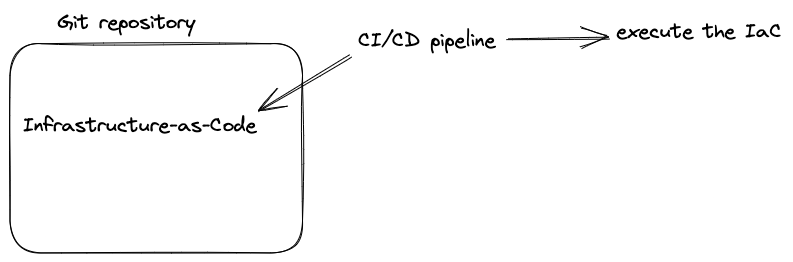
\includegraphics[width=1.00\linewidth]{assets/iac-is-not-gitops.png}
	\caption{IaC is not GitOps.
		%		(\citeauthor{ref}, \citeyear{ref}).
	}
	\label{fig:iacIsNotGitOps}	
\end{figure}

To avoid confusion with what GitOps actually is, 
the OpenGitOps project
\autocite{openGitOpsProject}
was created within the CNCF;
which is maintained by the GitOps working group.

The overall goal of OpenGitOps is to establish a clear vendor-neutral,
principle-driven meaning of GitOps,
which shall provide a foundation for interoperability between tools, conformance and certification through enduring programs, documents and code
\autocite{opengitopsDocuments}.

The definition of GitOps as per the OpenGitOps project
is stated in section \ref{theoretical-background:general-definitions} of this thesis.

In fig. \ref{fig:gitOpsConcept} a visual representation can be seen of the main GitOps concept.

\begin{figure}[h]
	\centering
	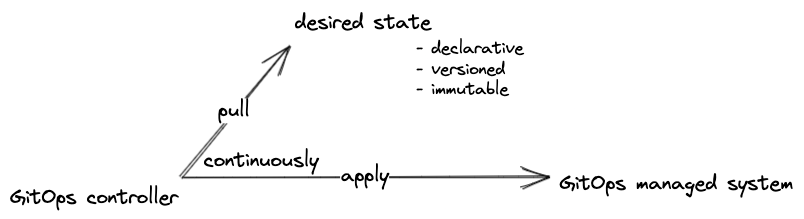
\includegraphics[width=1.00\linewidth]{assets/gitops-concept.png}
	\caption{GitOps concept.
		%		(\citeauthor{ref}, \citeyear{ref}).
	}
	\label{fig:gitOpsConcept}	
\end{figure}







\section{How GitOps changed Continuous Delivery}
\label{theoretical-background:gitops-cd}

Before GitOps, Continuous Delivery was primarliy push-based.
This means that a code change is introduced by a developer,
this code change is commited to a Git repository.
Then a CI/CD system gets triggered to execute a certain pipeline
of jobs.
These jobs may be to test the code and build an artifact, push the artifact
to a registry, etc.
The jobs are run in a pipeline - one after the other -
if one fails, the pipeline is cancelled.
The commit, that is a new version of the code -
is pushed through the pipeline.
Eventually at the end of the pipeline
the new version is deployed by pushing the new artifact
to the deployment environment in an imperative way.
Once the new version is deployed, the pipeline stops.

\begin{figure}[h]
	\centering
	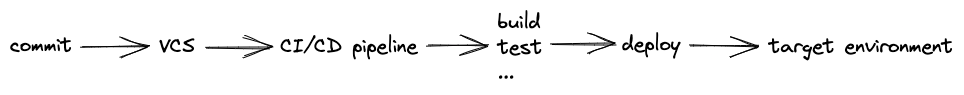
\includegraphics[width=1.00\linewidth]{assets/push-based-cd.png}
	\caption{Push based Continuous Delivery.
		%		(\citeauthor{ref}, \citeyear{ref}).
	}
	\label{fig:pushBasedCD}	
\end{figure}

With GitOps, this primarily push-based process has changed.
Namely, the last couple of steps when the new version
is deployed to the target environment,
are done asynchronously.
With a GitOps workflow,
the CI/CD pipeline usually stops when the new artifact
is successfully pushed to the artifact registry,
or the desired state is changed in the Git repository.
Then another system - the GitOps controller,
which usually lives inside the deployment environment -
notices that the desired state changed and has now
drifted from the actual state.
The GitOps controller then reconciles the new desired state,
by applying it to the managed system.

\begin{figure}[h]
	\centering
	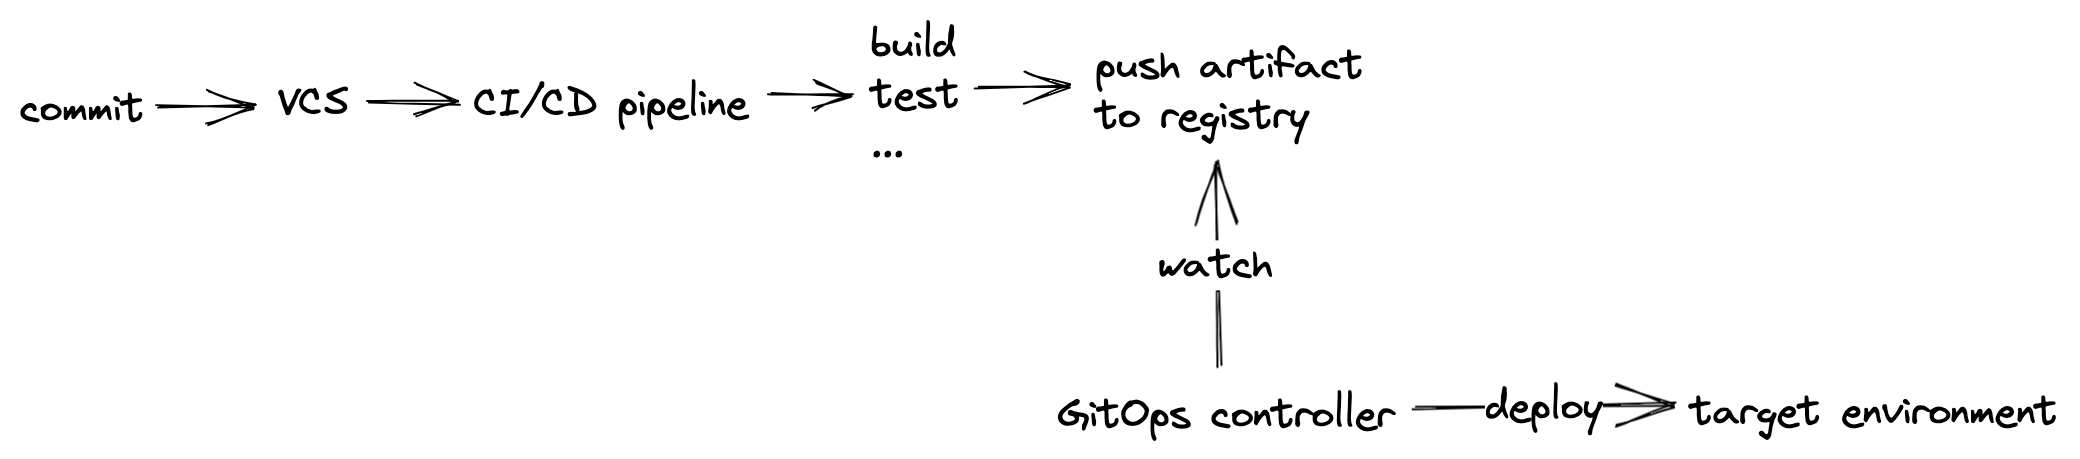
\includegraphics[width=1.00\linewidth]{assets/cd-gitops.png}
	\caption{Continuous Delivery with GitOps.
		%		(\citeauthor{ref}, \citeyear{ref}).
	}
	\label{fig:cd-gitops}	
\end{figure}

One major difference is that with the GitOps workflow,
the CI/CD system no longer knows if and where the application is being
deployed to, since the pipeline usually stops after successful push to the artifact registry.
The desired state, which is stored in a Git repository is continuously being watched
by the GitOps controller. Any changes that it detects are promptly applied to the
target environment.











\section{Promoting Releases Across Environments}

With the push-based pipelines, described in section
\ref{theoretical-background:gitops-cd},
it is typically more straight-forward of how an application
is deployed to multiple target environments.
When the pipeline job to deploy to environment A was successfully done,
the next job to deploy to environment B would be executed.
Since the push-based workflow was a synchronous process from commit
to deployment to target environment,
the whole process could be packed into a single pipeline.

However, with the GitOps workflow the process from
commit to deployment to target environment is usually split up after
publishing of the artifact to the artifact registry.
At this point, the process continues asynchronously.

There are multiple ways how the promotion across environments can be achieved.
In the simplest form, the desired state could be stored in a Git repository,
and the GitOps engine would synchronize every new commit, which is detected -
meaning each and every new change to the desired state is immediately
applied to the actual system state.
For each environment, there would be a representing folder in the Git repository,
or a separate repository.
On every new commit, the reconciliation immediately happens.
It could also be done differently, in that the state or source controller
is configured to watch a specific git refspec, meaning a certain Git tag, for example.
This way, not every commit is deployed, but rather only specific Git tags,
which may be created manually by a human.
When having the desired state as fixed Git tags,
it can possibly provide for more control over what is deployed.

Additionally to leveraging Git tags as fixed and immutable versions,
the desired state could be packaged and pushed to an artifact registry.
Especially when using configuration or templating tools like Kustomize or Helm,
where the Kubernetes manifests need to be rendered before being applied,
it could make sense to go with this approach.
Packaging the desired state into an immutable artifact can also increase
security, when the artifact is signed with a digital signature, and also validated upon deployment.

Whether the desired state is packaged as an artifact with an immutable version and signed signature,
or just stored in a Git repository and secured purely by the built-in Git commit functionality, providing
unique snapshots, which can be rolled back any time;
it always comes down to changing plain text files stored somewhere.
For promotion to other environments, these changes are typically done again for the desired state of the other environment.
There is no way around changing files in Git repositories, as this is within the nature of the GitOps approach.






\section{Towards Progressive Delivery \& Short-Living Environments}

With progressive delivery tools like
Flagger
\autocite{flaggerWebsite}
and
Argo Rollouts
\autocite{argoRolloutsWebsite},
which offer advanced deployment strategies
like canary and blue/green deployments, or A/B testing,
it is now easier to ensure a bad release does not impact the end users
as drastically.
As an example, the named tools make it possible to release new versions
to 10 percent of a specific region of end users,
then this canary rollout is automatically tested and evaluated against metrics,
if certain objectives for metrics fail to be met,
the new release can automatically be rolled back.

\begin{figure}[h]
	\centering
	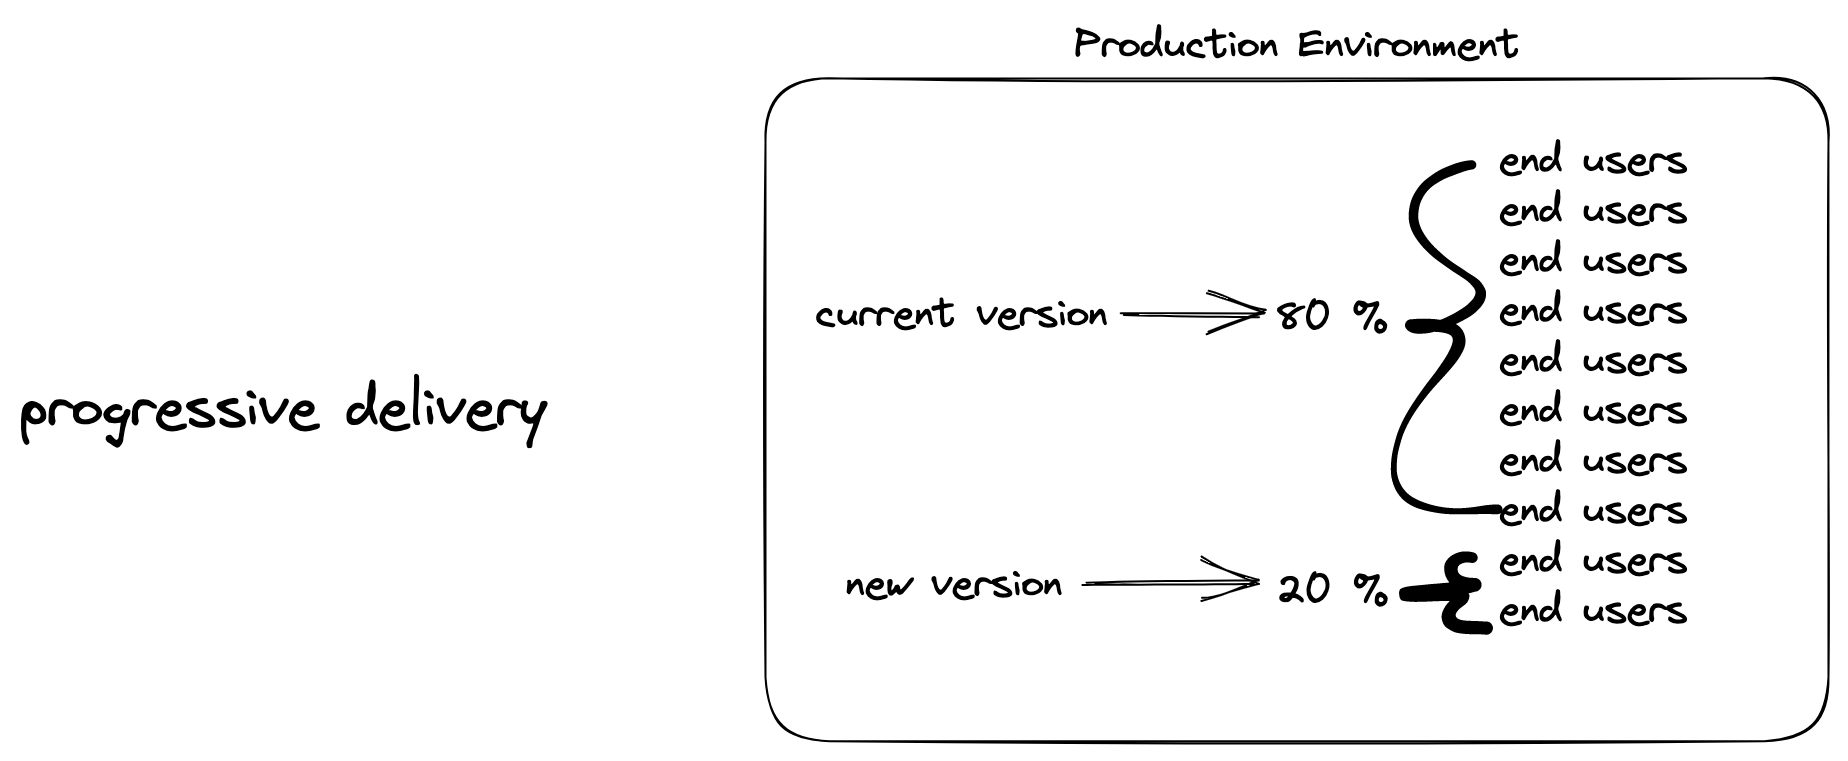
\includegraphics[width=1.00\linewidth]{assets/progressive-delivery.png}
	\caption{Progressive Delivery.
		%		(\citeauthor{ref}, \citeyear{ref}).
	}
	\label{fig:progressive-delivery}	
\end{figure}

Since the progressive delivery tools allow for a more
fine-grained segmentation
of a single environment based on numerous parameters like
client device type, user region, user type (e.g., developer, admin),
registered or unregistered users, etc.
the requirements to have a multitude of deployment environments
have decreased for some organizations.
An illustration can be seen in fig. \ref{fig:progressive-delivery}.

The described segmentation of an environment with the progressive delivery
tools, however might not be possible for every use case or organization.
Financial institutions for example, where the requirement for absolutely zero
errors hitting the production environment is top priority and business critical,
to say the least,
may still want to run multiple environments next to progressive delivery tools,
to ensure an even higher quality and level of caution.
This is illustrated in fig. \ref{fig:deploy-multiple-envs}.

Multiple environments typically mean a big increase in costs;
with progressive delivery the need for multiple environments has decreased,
and this way costs can be reduced.

\begin{figure}[h]
	\centering
	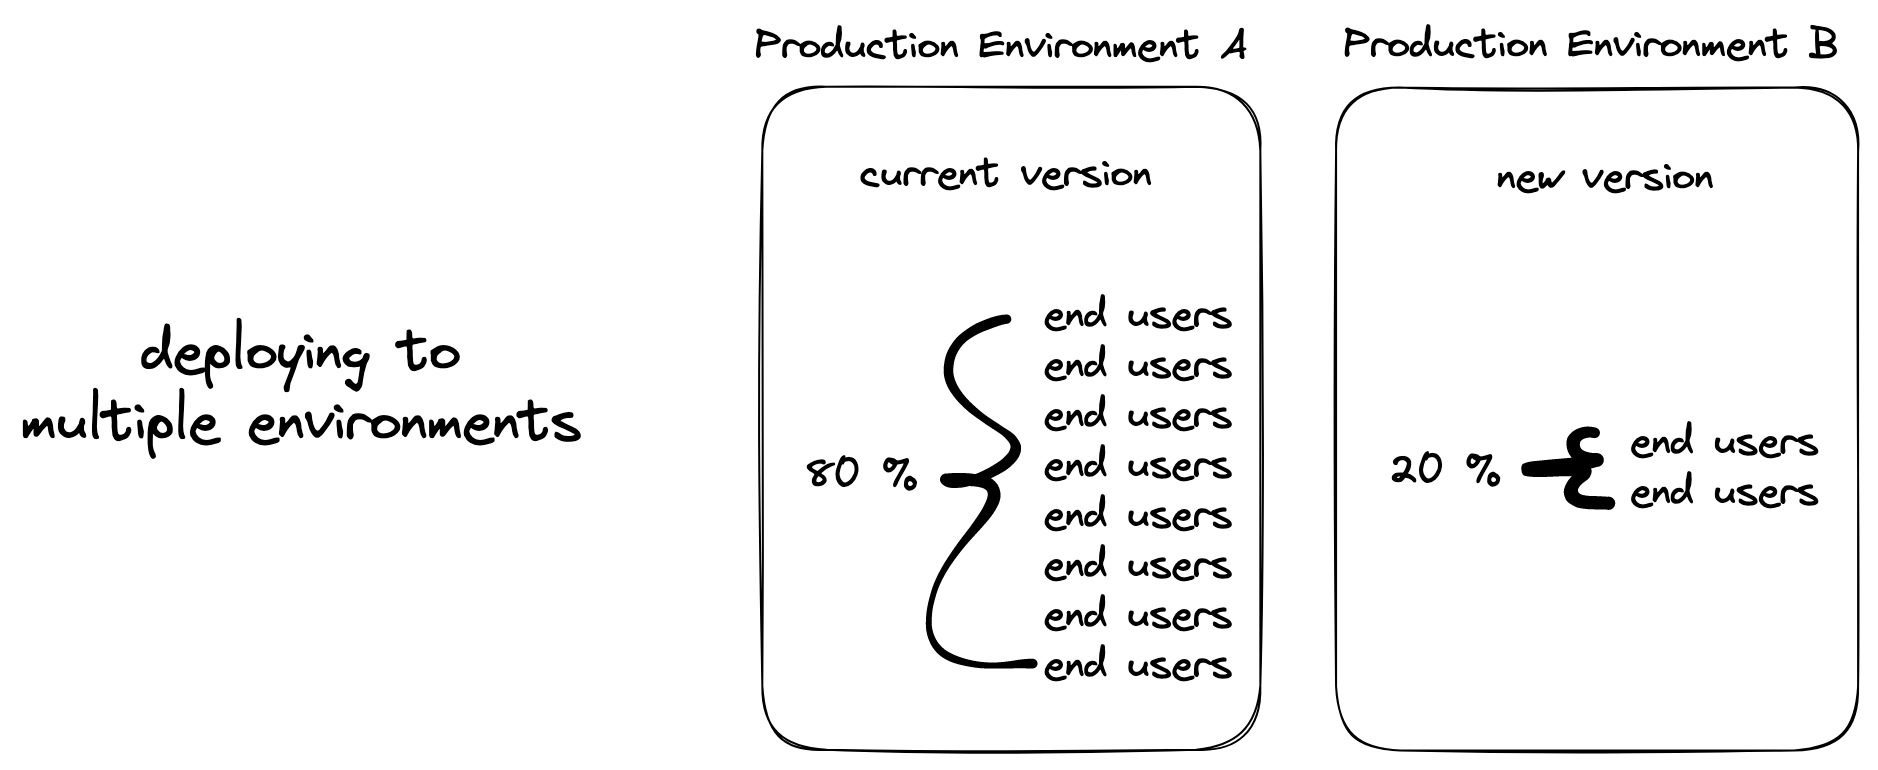
\includegraphics[width=1.00\linewidth]{assets/deploy-multiple-envs.png}
	\caption{Deploying to multiple environments.
		%		(\citeauthor{ref}, \citeyear{ref}).
	}
	\label{fig:deploy-multiple-envs}	
\end{figure}

Nowadays with the rapid development and releasing of new versions,
there has become a need for dynamic, short-living environments.
For every commit of an individual developer,
a deployment environment may be provisioned for previewing the changes
in a live environment that resembles the production environment as well as possible.
This short-living environment may be deleted after a short specified amount of time
has passed.






\section{Beyond container orchestration with Kubernetes}
\label{theoretical-background:kubernetes}

The following section is about
the role Kubernetes plays in the current cloud native ecosystem,
and its extensible architecture.

Since the birth of the cloud native computing foundation (CNCF) in 2015 and the release of Kubernetes as the first CNCF project,
there have emerged more than a hundred projects.
Most of the projects are hosting cloud native technologies and tools to support Kubernetes.
The current ecosystem and toolchains are strongly centered around Kubernetes,
although not strictly tied to it and often times with the explicit effort
for the ability to support alternative cloud native platforms and solutions.

\enquote*{Kubernetes, also known as K8s, is an open-source system for automating deployment, scaling, and management of containerized applications.}
\autocite{kubernetesIoWebsite}
Although this is the primary use case of Kubernetes,
and the reason why it was created initially,
Kubernetes is increasingly being used as a base cloud native platform,
to build other applications and platforms on top of.
The architecture of Kubernetes provides a solid framework and platform,
which is easily extensible.
Developers may extend its API by specifying custom resources and controllers.

There are several advantages when extending the Kubernetes API,
in comparison to a plain REST API.
Some of those are the following
\autocite{kubebuilderBookWebsite}:

\begin{itemize}
	\item \enquote*{Hosted API endpoints, storage, and validation.}
	\item \enquote*{Rich tooling and clis such as kubectl and kustomize.}
	\item \enquote*{Support for Authn and granular Authz.}
	\item \enquote*{Support for API evolution through API versioning and conversion.}
	\item \enquote*{Facilitation of adaptive / self-healing APIs that continuously respond to changes in the system state without user intervention.}
	\item \enquote*{Kubernetes as a hosting environment}
	\autocite{kubebuilderBookWebsite}
\end{itemize}

When developing a Kubernetes-native application,
many of the common capabilities which are often required for all applications,
are being provided by Kubernetes itself, or otherwise easily consumable and integrated.
These may include resource quotas, observability, monitoring, logging and tracing,
configuration state storage, declarative APIs, control loops, and event and message queueing.

\subsection*{Extending Kubernetes}
% https://kubernetes.io/docs/concepts/extend-kubernetes/
Kubernetes offers several different extension points and extension patterns.
Most extension patterns however share the same basic design and principles.
In general, a custom extension is a program which reads and/or writes
to the Kubernetes API. By doing that it can provide useful automation.
Since Kubernetes is based around a declarative API,
where resources are defined as the desired state,
and controllers are responsible for continuously reconciling this
desired state with the actual state,
it has shown to be a good pattern to design custom extensions in the same way
\autocite{extendKubernetes}.

\subsection*{Custom Resources, Controllers and Operators}
% https://kubernetes.io/docs/concepts/architecture/controller/
The concept of a controller and control loop within Kubernetes refers to the
meaning from robotics and automation, where
\enquote*{a control loop is a non-terminating loop that regulates the state of a system.}
\autocite{controllersKubernetes}
Controllers in Kubernetes are continuously running in a control loop,
in specified intervals and sometimes internal or external triggers, 
and watch the actual state of the cluster,
and make changes to it by interacting with the API,
in order to bring the actual state closer to the desired state,
like specified in the declarative definition.
It is typically a good practice to have one controller
be responsible for one resource, 
in order to help with separation of concerns.
Controllers make changes to resources inside the cluster,
like pods and deployments,
but can also be responsible for resources external to the cluster,
like APIs of the infrastructure provider
\autocite{controllersKubernetes}.
A typical controller implementation can be seen in figure
\ref{fig:typicalControllerKubernetes}.
As an example here, the deployment controller continuously ensures the desired state
of three replicas; if it notices the desired state and actual state differ
from one another, it does necessary actions to make them match again.

\begin{figure}[h]
	\centering
	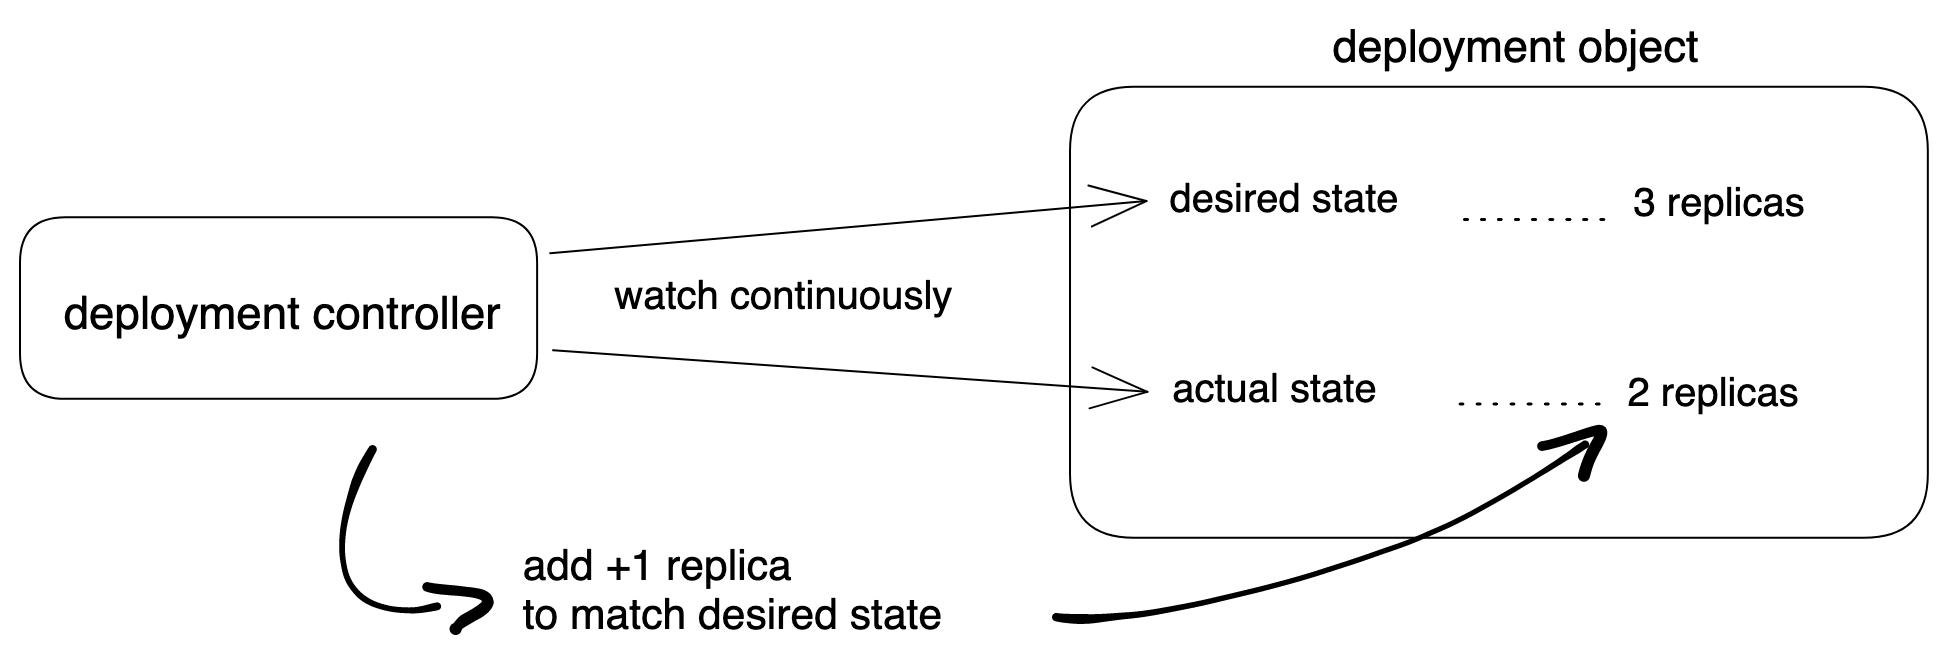
\includegraphics[width=1.00\linewidth]{assets/typical-controller.png}
	\caption{typical controller in Kubernetes.
		%		(\citeauthor{ref}, \citeyear{ref}).
	}
	\label{fig:typicalControllerKubernetes}	
\end{figure}

When a controller has specific domain knowledge,
or does certain tasks, which would usually be done by a human "operator",
it is called an operator.

% https://kubernetes.io/docs/concepts/extend-kubernetes/operator/
Operators typically are a set of controllers and custom resources
with specific codified domain knowledge.
All operational tasks -
which would otherwise have to be done by a human operator -
are written in code.
This code, the controller logic, can then be automated.
Examples for such operational tasks are
backups and restoring of backups, error remediation, database migrations, etc.
\autocite{operatorWhitepaperV1}.
In overly simplified terms:
An operator is a controller plus domain-specific operational knowledge
(fig. \ref{fig:operatorAndController}).

\begin{figure}[h]
	\centering
	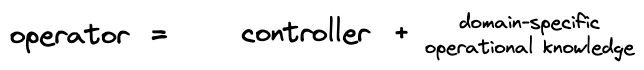
\includegraphics[width=0.85\linewidth]{assets/operator-is-controller-domain-knowledge.png}
	\caption{Operator and Controller.
		%		(\citeauthor{ref}, \citeyear{ref}).
	}
	\label{fig:operatorAndController}	
\end{figure}

The Operator Design Pattern represents a set of principles about
managing complex applications and/or infrastructure resources,
using domain-specific knowledge.
The goal is to limit any manual work that needs to be done,
and try to automate all operational tasks.
This is done by capturing domain-specific knowledge in code,
defining the desired state of resources and exposing them
via a declarative API
\autocite{operatorWhitepaperV1}.

To simplify the process of creating and maintaining Kubernetes-native application
in the form of an operator,
there exist several operator frameworks.
The most prominent framework is the Kubebuilder Framework.
%\url{https://github.com/kubernetes-sigs/kubebuilder}
The Kubebuilder framework makes the process of extending the Kubernetes API
an easy process for developers.
An initial project can easily be boostrapped, allowing the developer to focus
on implementing the custom resource definitions and controller logic.
Any needed Kubernetes primitives, such as service accounts and RBAC permissions
are automatically generated.
Documentation for the OpenAPI resources are also generated from the code,
which is the Go programming language.
There exist rich libraries for interfacing with Kubernetes components,
since Kubernetes itself is also implemented in the Go language
\autocite{kubebuilderBookWebsite}.

With custom resources, the Kubernetes API can dynamically be extended during runtime,
without the need to access its source code or recompile it.

While a resource is
\enquote*{an endpoint in the Kubernetes API that stores a collection of API objects of a certain kind}
\autocite{customResourcesKubernetesIO},
a custom resource is
\enquote*{an extension of the Kubernetes API that is not necessarily available in a default Kubernetes installation}
\autocite{customResourcesKubernetesIO}.
Custom resources can be dynamically registered and independently updated.
Users can interface with its objects as they do with the Kubernetes built-in resources
\autocite{customResourcesKubernetesIO}.









\section{Modeling GitOps Environments}

GitOps environments as defined in section
\ref{theoretical-background:general-definitions},
are currently being modeled using different approaches.
The most prominent approach is to have a folder in a Git repository
per environment. This is straight-forward and easily compatible with
the currently most used configuration and templating tools like Kustomize and Helm.
Promotion would be just a file copy operation from one to another file or folder.
For each environment, or only critical ones, there could be a completely separate Git repository.
Having a separate repository opens up the possibility to have a more strict separation of concerns,
regarding permissions and access rights.
Anyone who has access to a Git repository has read access to the entire repository tree.
While the write access could potentially be limited by administrators or maintainers
to certain folders, the read access will always be open for anyone who has access to the repository.

Another approach is to have a Git branch per environment.
Promotion would be a Git merge from one to another branch.
When taking this approach, and also having environment-specific configuration,
it is possible, when not being careful, that a merge conflict happens,
and the promotion would need to be solved manually.
However when this approach is purely used for the purpose of staging,
meaning environments are identical, but new releases are deployed to some environments first
after other ones,
it could provide a seamless way of promotion by solely leveraging the built-in merge mechanism in Git.
Branches can usually be restricted or limited to certain developers only,
which would make it easier to implement the access permissions than the previous folder-per-environment approach.

This research focuses primarily on the modeling of folder-per-environment.








\section{Promotion Strategies with Existing Tools}

There are many ways for achieving a promotion process when using the GitOps approach for the Continuous Delivery of
an application or any other infrastructure declared in code.
When a push-based CI/CD pipeline is already in place, it is often the first thing that comes to mind
to just append the GitOps deployment as a synchronized process to the end of the pipeline.
GitOps engines like ArgoCD offer the capability for the user to configure webhook receivers
which reconcile an application. This makes it possible to setup a synchronous pipeline,
which results in every code change being delivered through a pipeline step by step in a synchronous manner.
After the push-based synchronous deployment step succeeds in the pipeline process,
the pipeline developer can configure another imperative step which triggers reconcilication for another environment.

However, there is a downside when choosing to go with such a push-based imperative approach.
In fact, this approach would abide by the core principles of GitOps,
namely the principle of desired state being continuously being pulled by the GitOps engine/agent.
So the advantage of drift detection and automatic mending, would no longer be given.

When following the GitOps approach, it may be desirable to decouple Continuous Integration/Delivery and Continuous Deployment.
This means that a code change, namely a Git commit, triggers a Continuous Integration pipeline,
which ends in a step which builds and pushes an artifact of the new version to an artifact registry.
The pipeline ends at this point.
Afterwards the GitOps engine, another system than the CI/CD system, is responsible for detecting the new desired state and starting reconciliation.
However, the desired state first needs to be changed after a new artifact is available,
and especially when multiple environments are needed and promotion should be achieved between them,
this is not straight-forward with this asynchronous process.
It may be desirable to trigger tests after a deployment to a certain environment is done,
and only afterwards promote to another environment.
The GitOps approach proposes to have the source of truth in the Git repository as the desired state of a system.

Currently there is insufficient tooling in the GitOps ecosystem for streamlining such a
multi-environment promotion process.

{\color{red}\larger TODO review section!}



















\section{Summary}

TODO































%
%\section{Instruction included in the original FHBgld word processor template}
%\subsection{General definitions}
%Die in dieser Formatvorlage beispielhaft enthaltenen Überschriften sind auf die im
%konkreten Fall tatsächlich passenden Überschriften anzupassen.
%In diesem Teil der Arbeit werden die zum eindeutigen Verständnis unbedingt
%erforderlichen Grundlagen und Definitionen sowie die Erklärung wichtiger Begriffe
%angeführt.
%Die Gliederungspunkte müssen möglichst prägnant bezeichnet werden.
%\subsection{Related work / state of research}
%Auch die neuesten Entwicklungen und Arbeiten auf diesem Gebiet (Stand der
%Wissenschaft oder auch state-of-the-art) sind darzulegen, wobei diese je nach Thema
%auch in der 1. Gliederungsebene behandelt werden können.
%
%\section{Ordinary text}
%% A '%' character causes TeX to ignore all remaining text on the line,
%% and is used for comments like this one.
%
%% sections are begun with similar 
%% \subsection and \subsubsection commands.
%
%The ends  of words and sentences are marked by spaces. It doesn't matter how many 
%spaces    you type; one is as good as 100.  The
%end of   a line counts as a space.
%
%One   or more   blank lines denote the  end 
%of  a paragraph.  
%
%Since any number of consecutive spaces are treated
%like a single one, the formatting of the input
%file makes no difference to
%\LaTeX,                % The \LaTeX command generates the LaTeX logo.
%but it makes a difference to you.  When you use 
%\LaTeX \cite{lamport94},  % \cite inserts a reference, which you define at the end of the document
%making your input file as easy to read
%as possible will be a great help as you write 
%your document and when you change it.  This sample 
%file shows how you can add comments to your own input 
%file.
%
%Because printing is different from typewriting,
%there are a number of things that you have to do
%differently when preparing an input file than if
%you were just typing the document directly.
%Quotation marks like
%``this'' 
%have to be handled specially, as do quotes within
%quotes:
%``\,`this'            % \, separates the double and single quote.
%is what I just 
%wrote, not  `that'\,''.  
%
%Dashes come in three sizes: an 
%intra-word 
%dash, a medium dash for number ranges like 
%1--2, 
%and a punctuation 
%dash---like 
%this.
%
%A sentence-ending space should be larger than the
%space between words within a sentence.  You
%sometimes have to type special commands in
%conjunction with punctuation characters to get
%this right, as in the following sentence.
%Gnats, gnus, etc.\ all  % `\ ' makes an inter-word space.
%begin with G\@.         % \@ marks end-of-sentence punctuation.
%You should check the spaces after periods when
%reading your output to make sure you haven't
%forgotten any special cases.  Generating an
%ellipsis
%\ldots\               % `\ ' is needed after `\ldots' because TeX 
%% ignores spaces after command names like \ldots 
%% made from \ + letters.
%%
%% Note how a `%' character causes TeX to ignore 
%% the end of the input line, so these blank lines 
%% do not start a new paragraph.
%%
%with the right spacing around the periods requires
%a special command.
%
%\LaTeX\ interprets some common characters as
%commands, so you must type special commands to
%generate them.  These characters include the
%following:
%\$ \& \% \# \{ and \}.
%
%In printing, text is usually emphasized with an
%\emph{italic}  
%type style.  
%
%\begin{em}
%	A long segment of text can also be emphasized 
%	in this way.  Text within such a segment can be 
%	given \emph{additional} emphasis.
%\end{em}
%
%It is sometimes necessary to prevent \LaTeX\ from
%breaking a line where it might otherwise do so.
%This may be at a space, as between the ``Mr.''\ and
%``Jones'' in
%``Mr.~Jones'',        % ~ produces an unbreakable interword space.
%or within a word---especially when the word is a
%symbol like
%\mbox{\emph{itemnum}} 
%that makes little sense when hyphenated across
%lines.
%
%Footnotes\footnote{This is an example of a footnote.}
%pose no problem.
%
%\LaTeX\ is good at typesetting mathematical formulas
%like
%\( x-3y + z = 7 \) 
%or
%\( a_{1} > x^{2n} + y^{2n} > x' \)
%or  
%\( AB  = \sum_{i} a_{i} b_{i} \).
%The spaces you type in a formula are 
%ignored.  Remember that a letter like
%$x$                   % $ ... $  and  \( ... \)  are equivalent
%is a formula when it denotes a mathematical
%symbol, and it should be typed as one.
%Furthermore you can add a formula as Images or Tables, see Formula  \hyperref[eq:abc]{\ref{eq:abc}}
%\begin{equation}
%	\label{eq:abc}
%	a+b=c
%\end{equation}
%
%It is sometimes necessary to prevent \LaTeX\ from
%breaking a line where it might otherwise do so.
%This may be at a space, as between the ``Mr.''\ and
%``Jones'' in
%``Mr.~Jones'',        % ~ produces an unbreakable interword space.
%or within a word---especially when the word is a
%symbol like
%\mbox{\emph{itemnum}} 
%that makes little sense when hyphenated across
%lines.

%\chapter{Methodology}

In this chapter,
the methodological approach,
as well as
the used scientific research methods
are presented.


\section{Approach}
\label{methodology:approach}

To achieve the main goal of the thesis and answer the identified research questions,
a mix of different scientific methods will be used.
In order to help with the recognition and legitimization of the conducted research,
a commonly accepted framework, namely
the methodology for conducting design science (DS) research
in information systems (IS)
\autocite{designScienceResearchMethodologyForInformationSystemsResearch}
will be applied.
It consists of six activities
(illustrated in Figure \ref{fig:dsrmProcessReleasePromotionGitOps}):

\begin{itemize}
	\item \nameref{methodology:activity1}
	\item \nameref{methodology:activity2}
	\item \nameref{methodology:activity3}
	\item \nameref{methodology:activity4}
	\item \nameref{methodology:activity5}
	\item \nameref{methodology:activity6}
\end{itemize}

%Since the model allows for process iteration,
%it will be decided by the researcher
%whether, at the end of activity 5,
%to iterate back to activity 3 to try to improve the artifact.
The process is structured in a nominally sequential order.
For this concrete research,
the problem-centered initiation is chosen as the entry point,
thus the process will begin with activity 1.
Afterwards the research will proceed sequentially,
because the idea of the research resulted from observation of the problem
\autocite{designScienceResearchMethodologyForInformationSystemsResearch}.
\bigskip

% TODO: add activity 1-6 to illustration?

\begin{figure}[h]
	\centering
	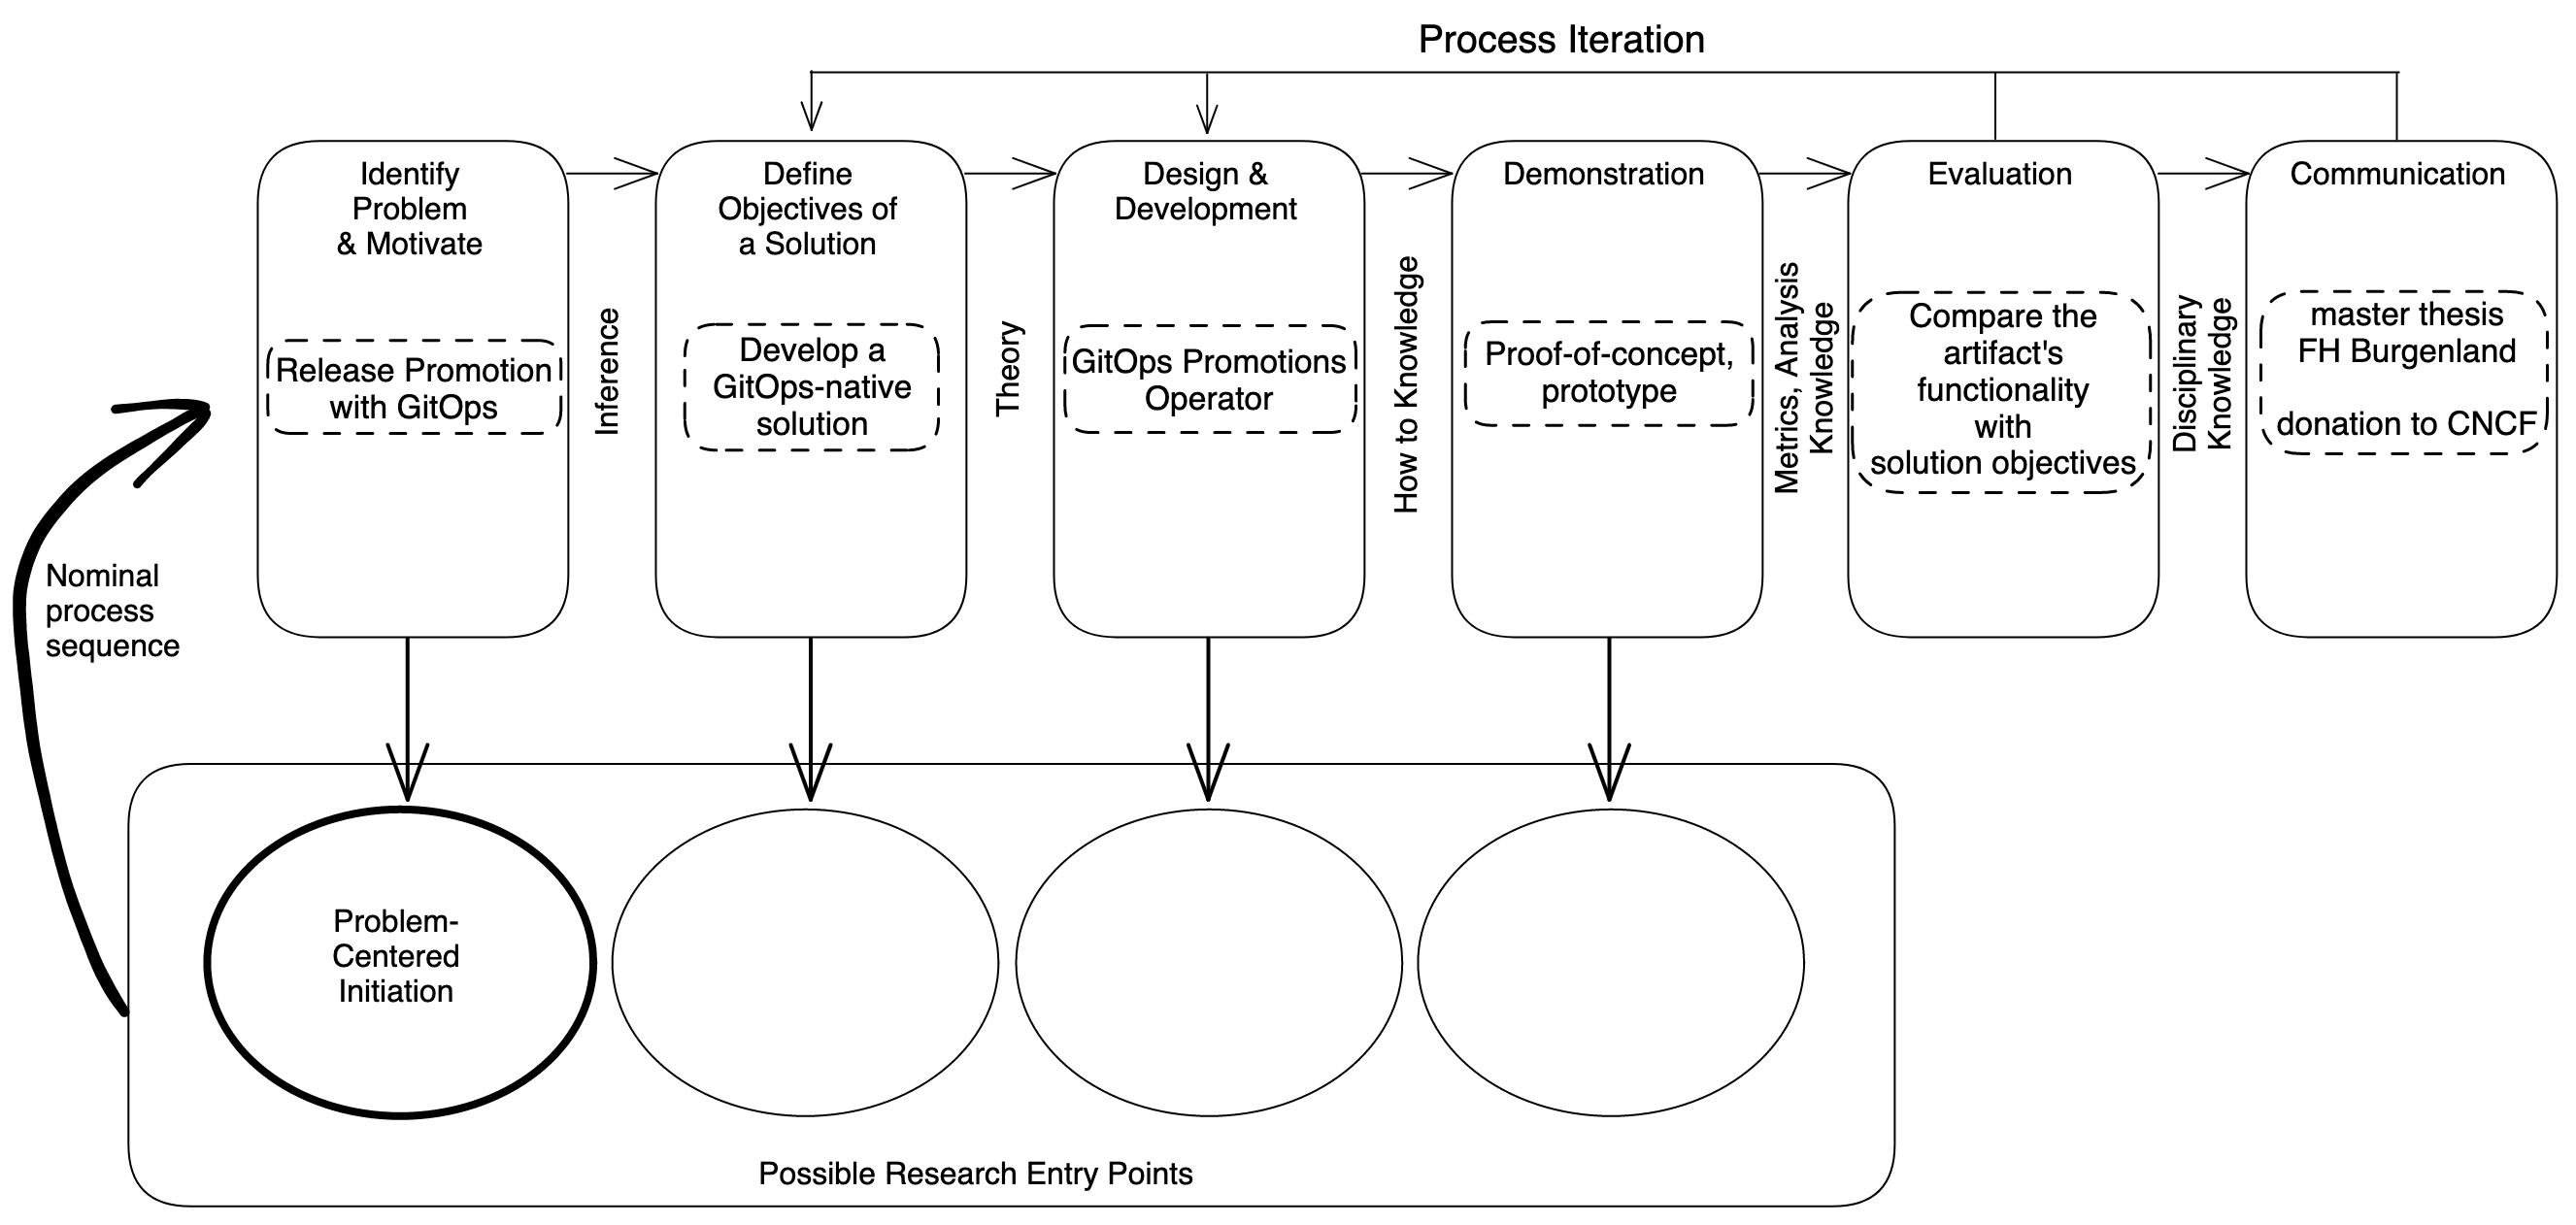
\includegraphics[width=1.00\linewidth]{figures/dsrm-process-release-promotion-gitops.png}
	\caption{DSRM Process for this thesis.
		%		(\citeauthor{ref}, \citeyear{ref}).
	}
	\label{fig:dsrmProcessReleasePromotionGitOps}	
\end{figure}

\subsection{Activity 1: Identify Problem \& Motivate}
\label{methodology:activity1}

\noindent
In activity 1,
the research problem of
release promotion with GitOps
is defined.
This is accomplished, by
seeking knowledge of the state of the problem
from practicing professionals.
This is done by conducting
semi-structured interviews, as described in section \ref{methodology:interview},
as well as analysing prior written literature.
To assist later evaluation,
the problem is conceptually broken down into distinct items.
The value of a solution is highlighted,
in order to help the audience of the research
understand the reasoning associated with the
researcher's understanding of the problem
\autocite{designScienceResearchMethodologyForInformationSystemsResearch}.
\bigskip

\begin{figure}[h]
	\centering
	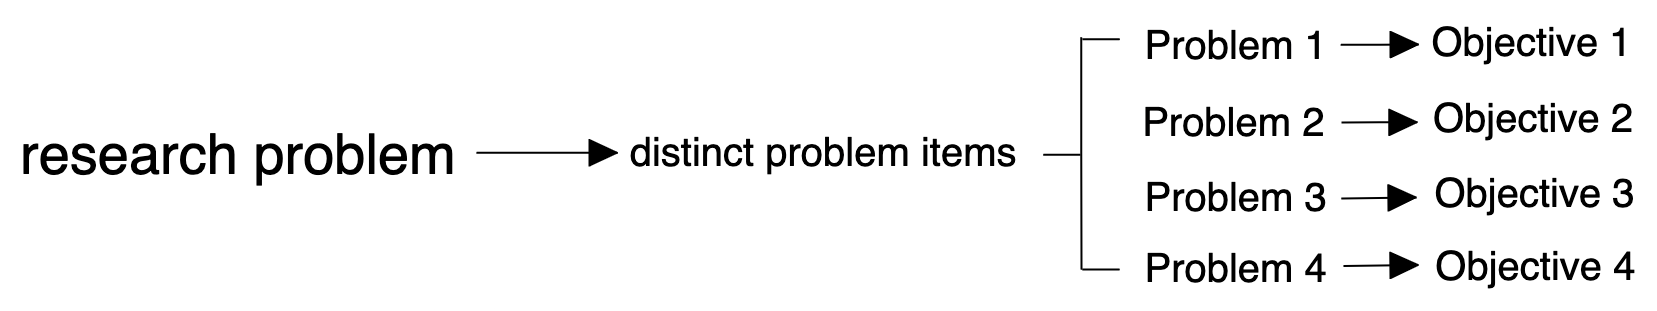
\includegraphics[width=0.75\linewidth]{assets/problem-to-objective-mapping.png}
	\caption{Inference of objectives from problems.
		%		(\citeauthor{ref}, \citeyear{ref}).
	}
	\label{fig:problemToObjectiveMapping}	
\end{figure}

\subsection{Activity 2: Define Objectives of a Solution}
\label{methodology:activity2}

\noindent
In activity 2,
research objectives are inferred from the problem definition in activity 1.
Each objective maps to a distinct item from the problem specification
(illustrated in Figure \ref{fig:problemToObjectiveMapping}),
which helps with later evaluation in activity 5.
In practice, a research objective will be a qualitative description of
how a new artifact is expected to support a solution to the problem definition.
\bigskip

\subsection{Activity 3: Design \& Development}
\label{methodology:activity3}

\noindent
In activity 3,
solutions for the previously defined objectives are designed and developed
by means of producing an artifact.
This is achieved by
determining the artifact's desired functionality and its architecture,
followed by actually creating the artifact
\autocite{designScienceResearchMethodologyForInformationSystemsResearch}.
In practice this means that:
Abstract model definitions are designed;
with the specification of the model definitions in place,
the "release promotion operator" is developed as an artifact.
\bigskip

\subsection{Activity 4: Demonstration}
\label{methodology:activity4}

\noindent
In activity 4,
the in-context use of the artifact is demonstrated.
After outlining how to use the artifact to effectively provide a solution to the problem definition,
the artifact is implemented in a proof-of-concept-level prototype.
%In practice,
%the prototype 
\bigskip

\subsection{Activity 5: Evaluation}
\label{methodology:activity5}

\noindent
In activity 5,
the implementation of the artifact,
and how well it supports a solution to the problem,
is evaluated.
This is achieved by
comparing the objectives of a solution to actual observed results
from use of the artifact in the demonstration
\autocite{designScienceResearchMethodologyForInformationSystemsResearch}.
In practice this means, that
the functionality of the artifact implemented in the prototype in activity 4,
is compared with the solution objectives from activity 2.
\bigskip

\subsection{Activity 6: Communication}
\label{methodology:activity6}

\noindent
In activity 6, as a final step,
the whole conducted research is communicated by means of
disclosing
the problem and its importance,
the artifact and its utility and novelty,
and the demonstration accompanied by the evalution results
\autocite{designScienceResearchMethodologyForInformationSystemsResearch},
within the publication of a master thesis at
the University of Applied Sciences Burgenland \autocite{fhBurgenlandWebsite}.
In addition, it is communicated to relevant audiences such as
the GitOps Working Group \autocite{gitopsWG} of the CNCF.






\section{Research methods}

In the following section,
the used research methods
semi-structured interview
by
\citeauthor{glaser2010experteninterviews} (\citeyear{glaser2010experteninterviews})
and
design science research methodology for information systems
by
\citeauthor{designScienceResearchMethodologyForInformationSystemsResearch} (\citeyear{designScienceResearchMethodologyForInformationSystemsResearch})
are explained in detail.
%The procedure in the course of the research work is also described.




\subsection{Semi-structured Interview}\label{methodology:interview}

For \nameref{methodology:activity1},
semi-structured interviews with working professionals
are conducted.
For this research method,
the suggested practices and guidelines from
the textbook of
\citeauthor{glaser2010experteninterviews} (\citeyear{glaser2010experteninterviews})
are used.
These interviews have the primary goal of aiding with
problem identification and motivation,
because prior written scientific literature is insufficient on the topic.
For conducting the interviews,
a semi-structured interview guide (Appendix \ref{appendix:interview-guide}) is used.

The interview guide is created on the basis of preliminary theoretical considerations.
The use of a guide facilitates the comparability of several interviews,
but still leaves enough room for spontaneous statements.
The advantage of a guide is that the researcher can stick to concrete questions.
Follow-up questioning is allowed and the questions are mostly open.
The open questioning enables the interviewee to present their point of view
\autocite{berger2016wissenschaftliches}.


\subsubsection*{Preparing the Interviews}

As an initial step,
a semi-structured interview guide is developed.
It serves as a rough guideline for the structure of the interview process.
Additionally it encompasses the content-related interview questions,
which are specific to the given research problem.
These questions can be seen at section \ref{appendix:interview-questions} in the appendix.

The selection of the interview partners is based on the questions mentioned in
\citeauthor{glaser2010experteninterviews} (\citeyear{glaser2010experteninterviews}):

\begin{itemize}
	\item Who has the information relevant to this work?
	\item Who can describe it precisely?
	\item Who is most willing to be interviewed?
	\item Who is available?
\end{itemize}

The pool of potential interview partners is mainly oriented around
contacts from friends and acquaintances,
who are working professionally in the GitOps field.
The contact to the interview partners is done via Slack \autocite{slackWebsite} or e-mail.
Prior to conducting the interview, the interview guide is sent to the interviewee.

\subsubsection*{Conducting the interviews}

Appointments for the interviews are made with each interview partner in advance. 
Eventually, the interview is conducted with a web video conferencing tool like Zoom \autocite{zoomWebsite}.
The interviews are recorded for later transcription.
The semi-structured interview guide
is used as a guideline for the interview process as a whole.
However, the actual structure of the interview may differ for each individual interview and according interview partner.

\subsubsection*{Transcription and post-processing of the interviews}

The output of the interviews are in the form of audio-video recordings.
These are transcribed word-for-word into a written form afterwards.
The transcriptions can be seen in Appendix \ref{appendix:interview-transcriptions}.
The content-related answers of the interview partners are taken into consideration
for \nameref{methodology:activity1}, and there further processed.





\subsection{Qualitative Content Analysis}

For \nameref{methodology:activity2},
the transcriptions of the interviews are evaluated with
the qualitative content analysis by
\citeauthor{mayring2019qualitative} (\citeyear{mayring2019qualitative}).

\subsubsection*{Object and research question}

The underlying object for the content analysis are
the conducted semi-structured interviews as described in section \ref{methodology:interview}.

The research questions are presented in the earlier section \ref{introduction:research-question}.

\subsubsection*{Approach}

As the main approach,
the inductive category formation
is chosen.
The first text passage is read,
then a category is formed,
and finally you proceed to the next passage.
For the next passage,
you decide if an existing category matches
or you need to form a new one.
This process continues until all text passages are handled.
At the end, similar categories may be merged together.

\subsubsection*{Coding}

Each text passage is labelled with the according category.

\subsubsection*{Review of categories}

About halfway through the coding process,
\citeauthor{mayring2019qualitative} (\citeyear{mayring2019qualitative})
advises to review the already formed categories.
The following questions may be asked:
Do they represent the content well?
Were they formed in an appropriate relation?
How do possible denotations look?
Could you merge certain categories?

\subsubsection*{Completion of coding process}

After reviewing the categories,
and taking appropriate measures,
the coding process is completed.

\subsubsection*{Reliability check}

Once coding is completed,
a reliability check is done.
How much do the results differ in replication?
This is achieved by letting another independent researcher
execute the coding process.

%Cohens's Kappa (1960)
%Krippendorff's Alpha (1970)

\subsubsection*{Evaluation and interpretation}

A possible way for evaluation would be to check frequencies.

How often does each of the categories occur in the data set?
What does this mean in terms of my research question?
How do my results relate to the existing state of research?













\subsection{Design Science Research Methodology}

The
design science research methodology (DSRM)
has already been described and applied in the earlier section
\ref{methodology:approach} \nameref{methodology:approach}
of this thesis.

\citeauthor{designScienceResearchMethodologyForInformationSystemsResearch} (\citeyear{designScienceResearchMethodologyForInformationSystemsResearch})
describe DSRM as follows:

\begin{quotation}
\noindent
We propose and develop a design science research methodology (DSRM) for the
production and presentation of DS research in IS. This effort contributes to IS research
by providing a commonly accepted framework for successfully carrying out DS research
and a mental model for its presentation. It may also help with the recognition
and legitimization of DS research and its objectives, processes, and outputs, and it
should help researchers to present research with reference to a commonly understood
framework, rather than justifying the research paradigm on an ad hoc basis with each
new paper.

\noindent
\autocite{designScienceResearchMethodologyForInformationSystemsResearch}
\end{quotation}

\enquote*{DS is of importance in a discipline oriented to the creation of successful artifacts.}
\autocite{designScienceResearchMethodologyForInformationSystemsResearch}


%DSRM provides a nominal process model consisting of six steps:
%problem identification and motivation, definition of the objectives for a solution, design and development, demonstration, evaluation, and communication


















%\section{Approach}
%Alle im durchgeführten Untersuchungen und Versuche müssen systematisch und
%nachvollziehbar sein. Daher ist die gewählte Vorgangsweise genau zu beschreiben
%und zu begründen. Es empfiehlt sich, dafür Literatur zum wissenschaftlichen Arbeiten
%heranzuziehen.
%
%\section{Research methods}
%Die eingesetzte Methoden (z.B. Online-Befragung, Inhaltsanalyse, Interviews) müssen
%ebenfalls nachvollziehbar beschrieben werden.
%Unterschiedliche Untersuchungsmethoden haben oft unterschiedliche Genauigkeit.
%Neben der Begründung und Beschreibung der Untersuchungsmethoden ist auch eine
%Begründung und Beschreibung der verwendeten Auswertungsmethoden bzw. dafür
%verwendete Software unerlässlich\footnote{Wenn der Abstand zwischen Fußnotentrennstrich und Fußnote zu groß wird, gehen Sie folgend vor:
%	Wählen Sie im Hauptmenü „Ansicht | Entwurf | Verweise | Notizen anzeigen |
%	Fußnotentrennlinie". Dann können Sie unnötige Leerzeichen entfernen.
%}.
%Wenn es ein Kapitel 3.2.1 gibt, muss es auch ein Kapitel 3.2.2 geben.

%\subsubsection{<<Überschrift 4. Ebene>>}
%4 Überschriftenebenen müssen reichen.
%
%
%\section{Displayed Text}
%Text is displayed by indenting it from the left
%margin.  Quotations are commonly displayed.  There
%are short quotations
%\begin{quote}
%	This is a short quotation.  It consists of a 
%	single paragraph of text.  See how it is formatted.
%\end{quote}
%and longer ones.
%\begin{quotation}
%	This is a longer quotation.  It consists of two
%	paragraphs of text, neither of which are
%	particularly interesting.
%	
%	This is the second paragraph of the quotation.  It
%	is just as dull as the first paragraph.
%\end{quotation}
%Another frequently-displayed structure is a list.
%The following is an example of an \emph{itemized}
%list.
%\begin{itemize}
%	\item This is the first item of an itemized list.
%	Each item in the list is marked with a ``tick''.
%	You don't have to worry about what kind of tick
%	mark is used.
%	
%	\item This is the second item of the list.  It
%	contains another list nested inside it.  The inner
%	list is an \emph{enumerated} list.
%	\begin{enumerate}
%		\item This is the first item of an enumerated 
%		list that is nested within the itemized list.
%		
%		\item This is the second item of the inner list.  
%		\LaTeX\ allows you to nest lists deeper than 
%		you really should.
%	\end{enumerate}
%	This is the rest of the second item of the outer
%	list.  It is no more interesting than any other
%	part of the item.
%	\item This is the third item of the list.
%\end{itemize}
%You can even display poetry.
%\begin{verse}
%	There is an environment 
%	for verse \\             % The \\ command separates lines
%	Whose features some poets % within a stanza.
%	will curse.   
%	
%	% One or more blank lines separate stanzas.
%	
%	For instead of making\\
%	Them do \emph{all} line breaking, \\
%	It allows them to put too many words on a line when they'd rather be 
%	forced to be terse.
%\end{verse}
%
%Mathematical formulas may also be displayed.  A
%displayed formula 
%is 
%one-line long; multiline
%formulas require special formatting instructions.
%\[  \Gamma \times  \psi = x'' + y^{2} + z_{i}^{n}\]
%Don't start a paragraph with a displayed equation,
%nor make one a paragraph by itself.

%%\chapter{Empirical Work}


\chapter{Interviews with Working Professionals}

\section{Problem Identification \& Motivation}
\section{Definition of Solution Objectives}
\section{Summary}



\chapter{GitOps Promotions Operator Prototype}

This chapter describes the developed prototype,
called the GitOps Promotions Operator.

\section{Design \& Development}

The Design of the GitOps Promotions Operator
is based on the underlying constraints of the Kubebuilder framework,
discussed in section \ref{theoretical-background:kubernetes} of this thesis.
The main constraints the framework comes with, are the
custom resource definition + controller pattern.

\begin{figure}[h]
	\centering
	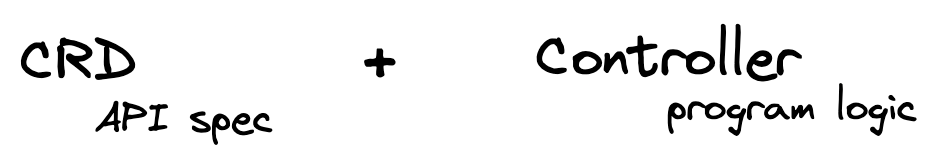
\includegraphics[width=1.00\linewidth]{assets/crd-and-controller.png}
	\caption{Custom Resource Definition and Controller.
		%		(\citeauthor{ref}, \citeyear{ref}).
	}
	\label{fig:crd-and-controller}	
\end{figure}

As the initial step of the design phase,
abstract model definitions are designed.
Their key properties are identified.
Then a sample mockup is designed as
a custom resource definition in Yaml format.
Afterwards this idea of the model definition is 
translated into custom struct types of the
Go programming language,
which is chosen by the Kubebuilder framework.

\subsection{Abstract Models}
	
The first step of the initial design phase is the creation of abstract models.
In order to be able to represent environments and promotions,
the requirement is to at least start with two abstract models for each 
the environment and promotion.

The Environment represents a GitOps environment,
which is a Git repository + path.
The Git repository can be a clone URL to the repository,
and the path is the relative filesystem path, which points to the 
environment, inside the repository.

\begin{figure}[h]
	\centering
	
\includegraphics[width=1.00\linewidth]{assets/gitops-env-repo-and-path.png}
	\caption{GitOps Environment.
		%		(\citeauthor{ref}, \citeyear{ref}).
	}
	\label{fig:gitops-env-repo-and-path}	
\end{figure}

The abstract model for a GitOps environment needs at least the following properties:

\begin{itemize}
	\item URL of the source Git repository
	\item path pointing to the environment inside the repository
\end{itemize}

The URL has the format of a HTTP(S) or SSH URL,
which links to the Git repository,
e.g.:

\begin{itemize}
	\item \lstinline|http://localhost:8080/org/repo|
	\item \lstinline|https://gitprovider.com/org/repo|
	\item \lstinline|ssh://git@gitprovider.com:org/repo|
\end{itemize}

The path has the format of a typical unix style filesystem path.
It starts relative from the root of the given Git repository,
and points to the directory, which represents the GitOps environment.
Examples for a path are the following:

\begin{itemize}
	\item \lstinline|path/to/env|
	\item \lstinline|/path/to/env|
	\item \lstinline|./path/to/env|
	\item \lstinline|./path/to/env/|
\end{itemize}

Note, that these example paths all represent the same directory,
these are just alternative notations.

The abstract model for a GitOps promotion needs at least the following properties:

\begin{itemize}
	\item source environment
	\item target environment
	\item promotion subjects
	\item promotion strategy
\end{itemize}

The source environment defines the environment resource,
where a promotion subject is promoted from.
The target environment defines the environment resource,
where a promotion should promote to.

A promotion subject can be potentially many different things.
In the case of this prototype,
a promotion subject is a file or directory,
which is copied from the source to the target environment.
Examples of such files or directories are the following:

\begin{itemize}
	\item \lstinline|kustomization.yaml|
	\item \lstinline|./component/cert-manager/kustomization.yaml|
	\item \lstinline|./helm-values-prod.yaml|
\end{itemize}

Note, that the relative paths of the promotion subjects,
are relative to the paths of the environment, defined earlier.
An example of the \lstinline|kustomization.yaml|, would look like this:

\lstinline|./path/to/env/kustomization.yaml|

As an example - but outside the scope of the current prototype -
a promotion subject could also be fetched from another source,
like an artifact registry, or be any other type of data
and updated/promoted in the target environment,
e.g. a version tag, helm values, etc.

With the current prototype,
the promotion strategy is to raise a pull request at the Git provider,
with the changes proposed by the promotion.
A human can then review the changes and optionally approve and merge the pull request.
After merging, the promotion will have taken place.

Alternatively to a pull request, the changes could be directly
commited and pushed to the target environment,
without human interaction. This strategy should require different means
of automated or otherwise external or additional checks, in order to ensure a safe promotion.

Now that the abstract models are designed,
they need to be implemented.
Since the decision for the prototype is to be developed
with the Kubebuilder framework and follow its style,
mockups of the custom resources in Yaml format
will be created as a next step.





\subsection{Mockups of Custom Resources}

%to write mockups
%of custom resources in YAML format,
%since this is what the end user will interface with when the application is finished.
%First and foremost the handling and user experience has to be seamless and make sense
%for the user; also it shouldn't take any extra miles for the user to take,
%just to get started.
%The YAML representation of the custom resource should be similar to other ones
%from the Kubernetes core types.

When the abstract models have been specified,
they can be actually implemented with the framework
as Kubernetes custom resource definitions.

Users will mainly be dealing with the custom resources in a Yaml format.
Yaml keys should be intuitive and make sense to the user.
It also helps if they follow the core Kubernetes definitions regarding naming conventions.
An example for a naming convention is the "Ref" suffix for yaml keys.
This suffix is typically appended to keys which represent a reference to another Kubernetes
object.
For example, "secretRef" says that this field refers to a Kubernetes secret resource.

A possible mockup for a GitOps environment -
that is a first prototype implementation of the abstract model into a custom resource -
could look like the following.

\lstinputlisting{assets/files/environment-mockup.yaml}

In this mockup the git reference branch main is also specified \\
in the \lstinline|.spec.source.ref.branch| field.

A possible mockup for a GitOps promotion 
could look like the following.

\lstinputlisting{assets/files/promotion-mockup.yaml}

In the promotion mockup definition,\\
there are four main fields within the \lstinline|.spec|.
These represent the minimum properties of the previously defined abstract definition.
It is to note, that
the \lstinline|.spec.copy| field represents the promotion subjects.
It is a list of items, where each item contains
a \lstinline|name|, \lstinline|source| and \lstinline|target|.
The \lstinline|name| defines a custom name.
The \lstinline|source| and \lstinline|target| fields together define a
file copy operation,
where the \lstinline|source| is the relative path from the source environment,
and the \lstinline|target| is a relative path from the target environment.

\subsection{Alternative Mockups}

The following alternative mockups,
for the custom resource definitions,
i.e. the design of the declarative API,
are suggested, but now implemented in the current prototype.

\subsubsection*{Promotion Subjects defined in each Environment resource}

Alternatively, the promotion subjects could also be specified
in the environment resource.
Then the environment could like the following:

\lstinputlisting{assets/files/environment-mockup-alt-1.yaml}

In the promotion definition,
it would then suffice to specify
a list of promotion subjects.

\lstinputlisting{assets/files/promotion-mockup-alt-1.yaml}

This alternative design allows that each environment could have
a unique path of a specific promotion subject defined.
Now if a promotion is spanning over multiple environments,
they could each specify their own unique path to a promotion subject.
The promotion subject is declared in the promotion,
but the actual path is defined per each environment.

\subsection{Translation to Go types}

Once the mockups of the custom resources in Yaml format are done,
the declarative structure can be translated to custom Go types.

The specification of the Environment resource results in the following code:

\lstinputlisting{assets/files/environmentSpec-type.go}

The type EnvironmentSpec represents the \lstinline|.spec| Yaml field.

What also needs to be defined is the status subresource.
In the status fields, the controller can save the current/actual state
of the resource during runtime.
While \lstinline|.spec| defines the desired state,
\lstinline|.status| defines the actual state, as observed by the controller.

% TODO: maybe show example of .status yaml

\lstinputlisting{assets/files/environmentStatusSpec-type.go}

The specification of the Promotion resource results in the following code:

\lstinputlisting{assets/files/promotionSpec-type.go}

For the promotion,
a status subresource is also defined.
In the status - the actual state of the resource as observed by the controller -
most importantly the metadata of the currently opened pull request is saved,
which the controller will pick up on every consecutive reconciliation
of the same promotion object.

\lstinputlisting{assets/files/promotionStatusSpec-type.go}

The full source code of the types can be found in Appendix
\ref{appendix:source-code}.

Once the Go types are defined,
the controller logic can be written.

\subsection{Controller Logic}

For the environment API,
a controller is written.
For this prototype the following logic was implemented.
First, the source git repository is cloned and checked out,
with the appropriate authentication options, if it is private.
If it succeeds, the Ready condition is set in the status subresource,
which will mark it available and ready for the promotion.

\begin{enumerate}
	\item test the clone of Git repository with authentication
	\item checkout reference branch locally
	\item mark environment as ready
\end{enumerate}

For the promotion API,
the following controller logic is implemented.
First, the controller checks if the source and target environments are ready,
if they are not yet ready, the controller cancels the reconciliation immediately.
Then the source and target environments are cloned.
Next the controller checks if there is a pending/open pull request,
this information is retrieved from the object's status, and then checked
if still up to date via the Git provider's API.
Afterwards the controller executes the promotion tasks,
which are the copy operations with the current state of the prototype.
Now if there were changes since the last reconciliation, the new commits
are pushed to the pull request branch.
Lastly, a pull request will be raised, if not yet done during a previous reconciliation.

\begin{enumerate}
	\item ensure that the source and target environments are ready
	\item clone source and target repositories
	\item check for a pending promotion (open Pull Request)
	\item execute the promotion copy operations
	\item push new commits to PR branch, if there were differences between source \& target environments
	\item create new PR, if not yet opened
\end{enumerate}

The full source code of the controllers can be found in Appendix
\ref{appendix:source-code}.






\section{Proof Of Concept Demonstration}

The following section demonstrates the in-context usage of the
developed prototype - the GitOps Promotions Operator - in a proof of concept.
The use case described as follows is created for the purpose of this demonstration.

This use case deals with a setup with multiple deployment environments.
There are two non-critical environments \lstinline|dev| and \lstinline|qa|,
and two production environments \lstinline|prod-1| and \lstinline|prod-2|.
The GitOps definitions of the non-critical environments are living inside the same
Git repository \lstinline|mtpoc-infra-1|,
and each production environment lives in its own separate Git repository
\lstinline|mtpoc-infra-2| for \lstinline|prod-1|,
and \lstinline|mtpoc-infra-3| for \lstinline|prod-2|.
In general, the application version shall be promoted with a strict flow
through the environments, one after the other.
An overview of the given setup can be seen in the table \ref{table:poc-environments-setup}.

\begin{table}[h]
\begin{center}
	\begin{tabular}{||c c c||} 
		\hline
		Order & Environment & Source Repository \\ [0.5ex] 
		\hline\hline
		1 & dev & mtpoc-infra-1 \\ 
		\hline
		2 & qa & mtpoc-infra-1 \\
		\hline
		3 & prod-1 & mtpoc-infra-2 \\
		\hline
		4 & prod-2 & mtpoc-infra-3 \\ [1ex]
		\hline
	\end{tabular}
	\caption{PoC Environments Setup}
	\label{table:poc-environments-setup}
\end{center}
\end{table}

The GitOps environment is centered around the used configuration management tool
Kustomize, and generally structured for all environments as below:

\begin{lstlisting}
.
|-- app-version
|   `-- kustomization.yaml
|-- kustomization.yaml
`-- settings
    `-- deployment.yaml
\end{lstlisting}

This structure adheres to the constraints of the currently available
copy operation promotion type, which can copy files and directories.
This means the configuration components which need to be promoted,
should be defined in separate files or directories.
This is needed, in order to only promote e.g. the application image version,
while leaving other configuration untouched, and specific to an environment.
With the Kustomize configuration tool, it is possible to split
parts of the main \lstinline|kustomization.yaml| into other separated files,
with the components feature.

In this use case, the value of the application's image version lives within the 
app-version component. This is configured in the main \lstinline|kustomization.yaml|
like this:

\begin{lstlisting}
components:
- app-version
\end{lstlisting}

The \lstinline|./app-version| directory contains a \lstinline|kustomization.yaml| file,
with typical Kustomization specification.
In this case, the images feature of Kustomize is used for configuring the application's
image version tag.

\begin{lstlisting}
apiVersion: kustomize.config.k8s.io/v1alpha1
kind: Component
images:
- name: ghcr.io/stefanprodan/podinfo
newTag: 6.3.4
\end{lstlisting}

Now the goal is to configure a promotion for the app-version component.
To achieve this, 
first, a \lstinline|Environment| resource needs to be created
for all environments respectively.
Only the \lstinline|dev| environment is shown here,
the other three environment definitions follow the same schema,
but are omitted for the sake of brevity.

\lstinputlisting{assets/files/dev-environment.yaml}

%\lstinputlisting{assets/files/qa-environment.yaml}
%
%\lstinputlisting{assets/files/prod-1-environment.yaml}
%
%\lstinputlisting{assets/files/prod-2-environment.yaml}

Now the specified secrets must be created.
The API token is required for the creation of pull requests by the promotion controller;
it must be stored in a Kubernetes generic secret resource in a key named \lstinline|token|,
and can be created with the following command:

\lstinline|kubectl create secret generic github-api-token --from-literal=token="gh..."|

With the current prototype, also a secret for the SSH connection to push and pull
the repository, needs to be created.
For this, a ssh key pair needs to be created by the user. Its public key needs to 
be set as a deploy key at the Git provider,
and its private key needs to be stored in a
Kubernetes generic secret resource in a key named \lstinline|private|.

\lstinline|kubectl create secret generic github-api-token --from-literal=private="--..."|

When all the four environments are created, the \lstinline|Promotion| resources
can be defined.
In this use case, three promotion resources are needed for the ability to
promote between all four environments with a straight flow - promoting from one to the next.
Only the \lstinline|dev-to-qa| promotion is shown here,
the other two definitions follow the same schema,
but are omitted here for the sake of brevity.

\lstinputlisting{assets/files/dev-to-qa.yaml}

%\lstinputlisting{assets/files/qa-to-prod-1.yaml}
%
%\lstinputlisting{assets/files/prod-1-to-prod-2.yaml}





At this point, all which is needed for promoting is configured.
When the status of all the environment resources involved in a promotion,
have a ready status condition,
a promotion will trigger.

\lstinputlisting{assets/files/env-dev-status.yaml}

At this point, the controller logs can be observed.

\begin{lstlisting}
2023-04-16T12:10:40Z    INFO    Begin reconciling Promotion     {"controller": "promotion", "controllerGroup": "promotions.gitopsprom.io", "controllerKind": "Promotion", "Promotion": {"name":"dev-to-qa","namespace":"default"}, "namespace": "default", "name": "dev-to-qa", "reconcileID": "ba3775ae-d8b1-40de-ad7b-4f42f8534686", "name": {"namespace": "default", "name": "dev-to-qa"}}
2023-04-16T12:10:46Z    INFO    Created new pull request        {"controller": "promotion", "controllerGroup": "promotions.gitopsprom.io", "controllerKind": "Promotion", "Promotion": {"name":"dev-to-qa","namespace":"default"}, "namespace": "default", "name": "dev-to-qa", "reconcileID": "ba3775ae-d8b1-40de-ad7b-4f42f8534686", "WebURL": "https://github.com/thomasstxyz/mtpoc-infra-1/pull/1"}
2023-04-16T12:10:46Z    INFO    Reconciled Promotion successfully       {"controller": "promotion", "controllerGroup": "promotions.gitopsprom.io", "controllerKind": "Promotion", "Promotion": {"name":"dev-to-qa","namespace":"default"}, "namespace": "default", "name": "dev-to-qa", "reconcileID": "ba3775ae-d8b1-40de-ad7b-4f42f8534686", "duration": "6.050374419s", "nextReconcile": "300s"}
\end{lstlisting}

A new pull request
%with the number \lstinline|1|
%at the Web URL \\
%\url{https://github.com/thomasstxyz/mtpoc-infra-1/pull/1} \\
has been created by the controller.

The promotion's status will also reflect, that
a pull request is open for review.

\lstinputlisting{assets/files/prom-dev-to-qa-status.yaml}

The open pull request is ready for review in the Git provider's web interface.
%\begin{figure}[h]
%	\centering
%	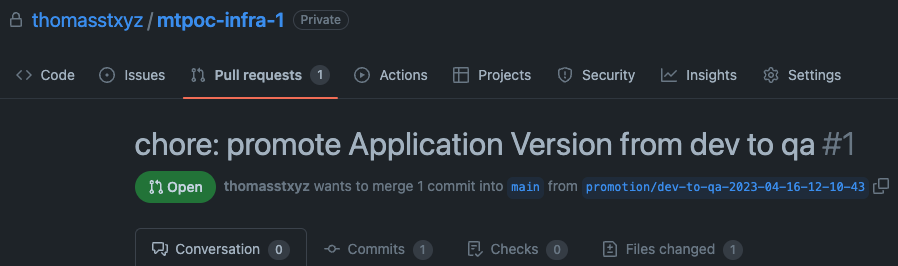
\includegraphics[width=1.00\linewidth]{assets/new-promotion-github.png}
%	\caption{New Git Pull Request.
%		%		(\citeauthor{ref}, \citeyear{ref}).
%	}
%	\label{fig:new-promotion-github}	
%\end{figure}
\begin{figure}[h]
	\centering
	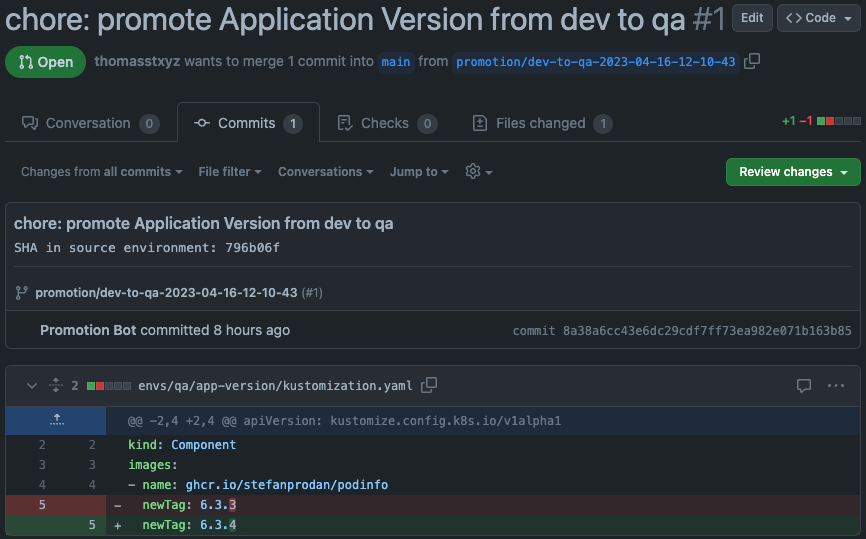
\includegraphics[width=1.00\linewidth]{assets/prom-pr-dev-to-qa.png}
	\caption{Pull Request for Promotion from dev to qa.
		%		(\citeauthor{ref}, \citeyear{ref}).
	}
	\label{fig:prom-pr-dev-to-qa}	
\end{figure}

The changed difference introduced by the commit can be viewed:

\begin{lstlisting}
- newTag: 6.3.3
+ newTag: 6.3.4
\end{lstlisting}

The \lstinline|dev-to-qa| promotion requested the change of the image version from
\lstinline|6.3.3| to \lstinline|6.3.4|.

Now, since the \lstinline|qa| and the \lstinline|prod-1| environments
also differ,
a pull request has also been created for this promotion.

%\begin{figure}[h]
%	\centering
%	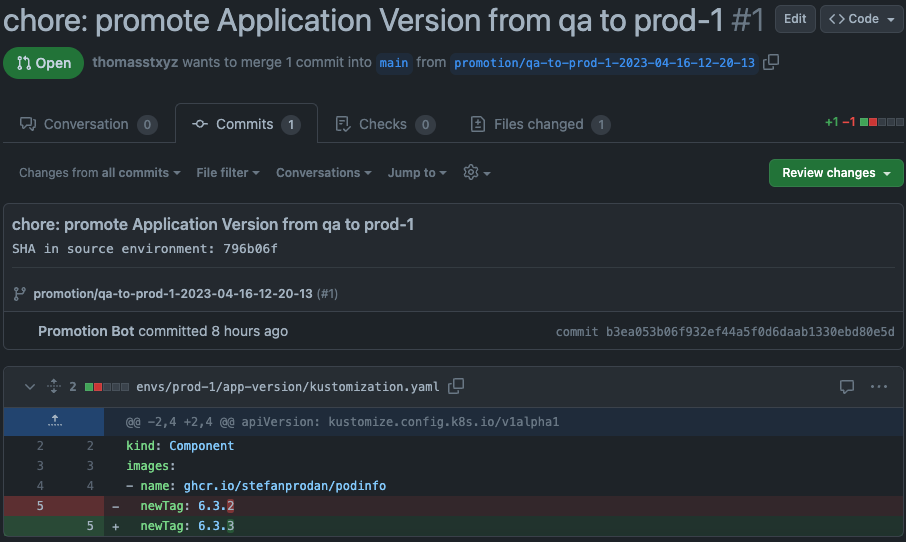
\includegraphics[width=1.00\linewidth]{assets/prom-pr-qa-to-prod-1.png}
%	\caption{Pull Request for Promotion from qa to prod-1.
%		%		(\citeauthor{ref}, \citeyear{ref}).
%	}
%	\label{fig:prom-pr-qa-to-prod-1}	
%\end{figure}

The \lstinline|qa-to-prod-1| promotion requested the change of the image version from
\lstinline|6.3.2| to \lstinline|6.3.3|.

\begin{lstlisting}
- newTag: 6.3.2
+ newTag: 6.3.3
\end{lstlisting}

Now, since the \lstinline|prod-1| and the \lstinline|prod-2| environments
also differ,
a pull request has also been created for this promotion.

%\begin{figure}[h]
%	\centering
%	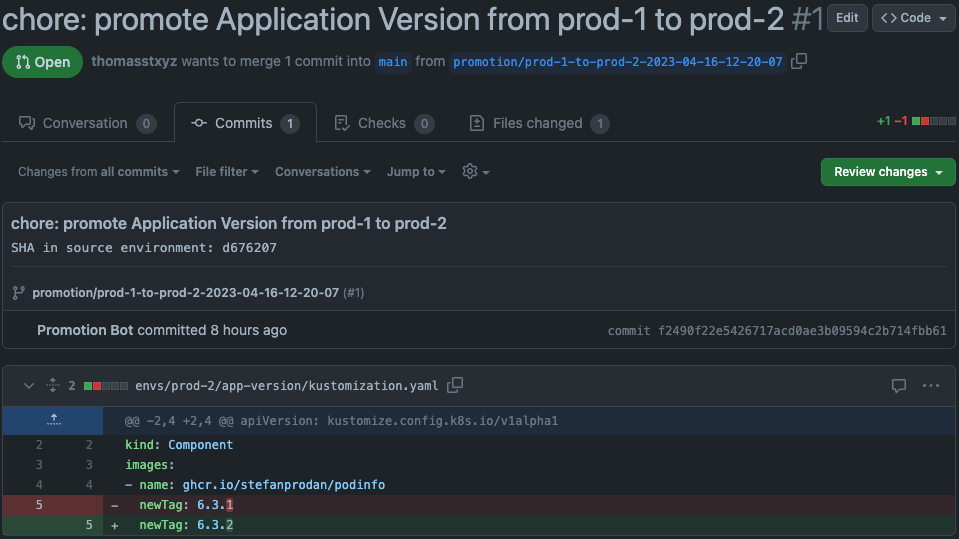
\includegraphics[width=1.00\linewidth]{assets/prom-pr-prod-1-to-prod-2.png}
%	\caption{Pull Request for Promotion from prod-1 to prod-2.
%		%		(\citeauthor{ref}, \citeyear{ref}).
%	}
%	\label{fig:prom-pr-prod-1-to-prod-2}	
%\end{figure}

The \lstinline|prod-1-to-prod-2| promotion requested the change of the image version from
\lstinline|6.3.1| to \lstinline|6.3.2|.

\begin{lstlisting}
- newTag: 6.3.1
+ newTag: 6.3.2
\end{lstlisting}

If the \lstinline|dev| environment advances the application image version further,
the pull request for the \lstinline|dev-to-qa| will be updated with another commit.
Note that the previous commit is not overwritten, 
but the commit history is kept on the pull request branch - now there are two commits on the branch.

\begin{figure}[h]
	\centering
	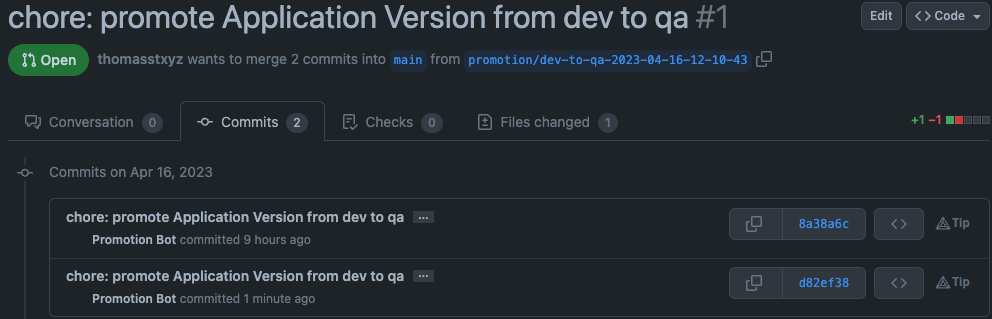
\includegraphics[width=1.00\linewidth]{assets/prom-pr-dev-to-qa-round2.png}
	\caption{Pull Request updated for Promotion from dev to qa.
		%		(\citeauthor{ref}, \citeyear{ref}).
	}
	\label{fig:prom-pr-dev-to-qa-round2}	
\end{figure}

The difference for the \lstinline|dev-to-qa| promotion is now:

\begin{lstlisting}
- newTag: 6.3.3
+ newTag: 6.3.5
\end{lstlisting}

%\begin{figure}[h]
%	\centering
%	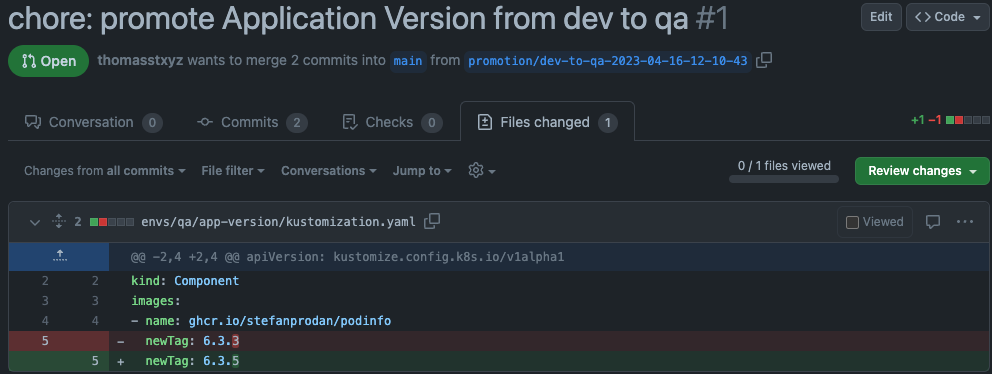
\includegraphics[width=1.00\linewidth]{assets/prom-pr-dev-to-qa-round2-diff.png}
%	\caption{Pull Request updated for Promotion from dev to qa (diff).
%		%		(\citeauthor{ref}, \citeyear{ref}).
%	}
%	\label{fig:prom-pr-dev-to-qa-round2-diff}	
%\end{figure}

Now if the pull request for the \lstinline|dev-to-qa| promotion
is approved and merged by a human,
the promotion will actually take effect.
This will results in the \lstinline|qa-to-prod-1| promotion pull request being updated
by the promotion controller.
Version \lstinline|6.3.5| is now requested for promotion to the
\lstinline|prod-1| environment.

The difference for the \lstinline|qa-to-prod-1| promotion is now:

\begin{lstlisting}
- newTag: 6.3.2
+ newTag: 6.3.5
\end{lstlisting}

Once reviewed, approved and merged by a human,
the promotion of version \lstinline|6.3.5| to the \lstinline|prod-1| environment
will result in further propagation of version \lstinline|6.3.5|
to the \lstinline|prod-2| environment.

The difference for the \lstinline|prod-1-to-prod-2| promotion pull request is now:

\begin{lstlisting}
- newTag: 6.3.1
+ newTag: 6.3.5
\end{lstlisting}

Once reviewed, approved and merged by a human,
the promotion of version \lstinline|6.3.5| to the \lstinline|prod-2| environment
will take effect.

The described demonstration showed,
how an application version can be promoted across multiple environments,
while ensuring a strict flow of promotion of \\
e.g. \lstinline|dev --> qa --> prod-1 --> prod-2|




%For this demonstration, it is supposed that
%the latest version \lstinline|6.3.5| is bad and should not be promoted,
%instead the \lstinline|dev| environment shall be rolled back to \lstinline|6.3.4|.






















\section{Evaluation Of Proof-of-Concept Use Cases}











\section{Summary}







%\chapter{Interviews with Working Professionals}
%
%\section{Categorisation of Findings}
%\section{Common Problem Definitions}
%\section{...?}
%
%
%\chapter{Definition of Solution Objectives}
%
%\section{People \& Communication Perspective}
%\section{Technical Perspective}
%\section{...?}
%
%
%\chapter{Prototype Design and Development}
%
%\section{Architecture}
%\section{Functionality}
%\section{...?}
%
%\chapter{Proof-of-Concept Demonstration}
%
%\section{Setup and Use with Kustomize}
%\section{Setup and Use with Helm}
%\section{Multiple Environments in same Stage}
%\section{Scalability}
%\section{...?}















%
%\section{Instruction included in the original FHBgld word processor template}
%Die Durchführung der empirischen Untersuchung ist nachvollziehbar zu dokumentieren sowie auch die dabei aufgetretenen Probleme und deren Behandlung. Der Umfang ergibt sich aus der Art der Bearbeitung.  
%
%Tabelle 1 zeigt ein Bespiel für eine Tabelle. 
%
%\begin{figure}[ht]
%	\centering
%	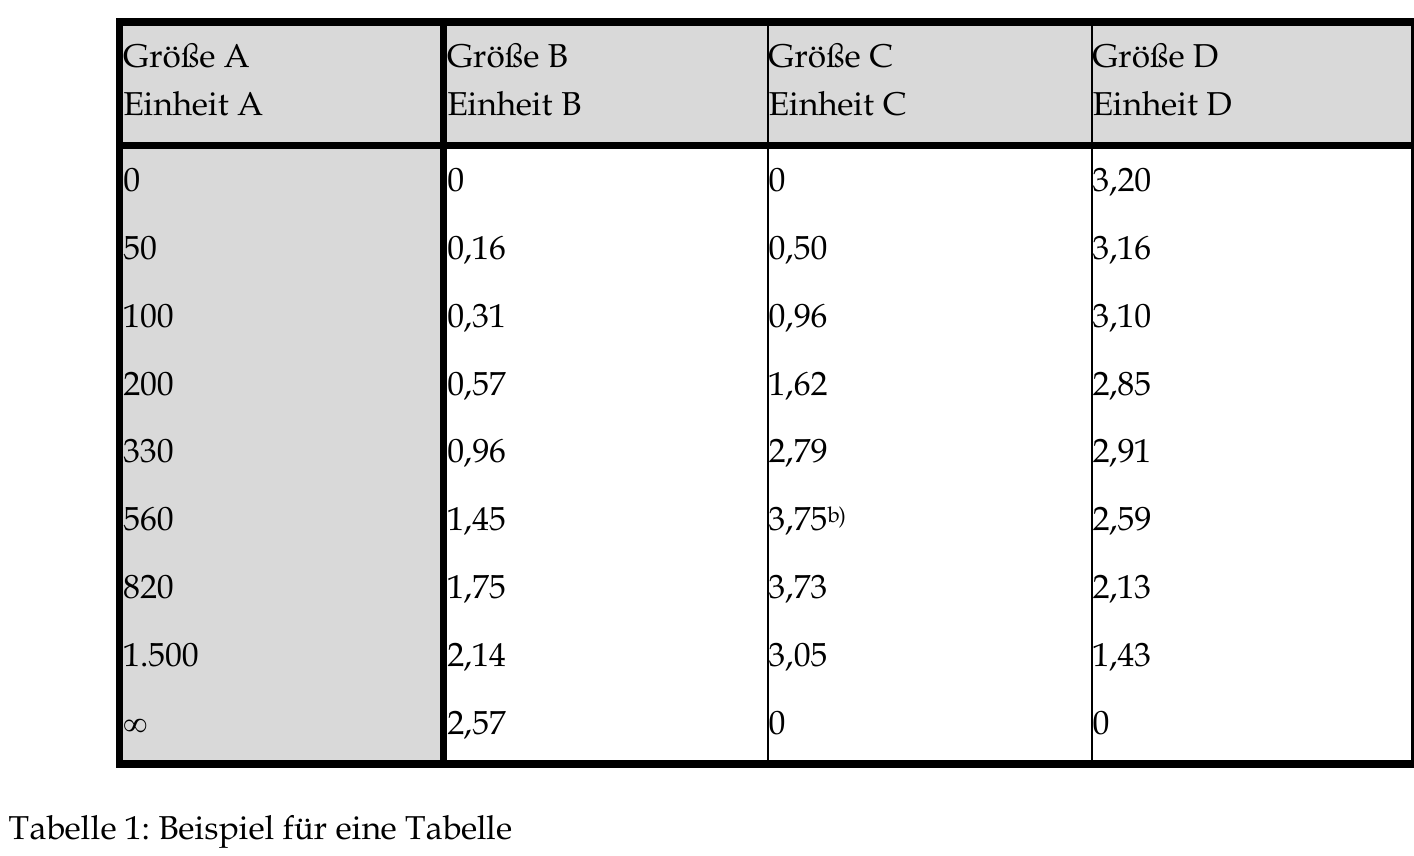
\includegraphics[width=0.7\linewidth]{figures/Word_Table}
%	\caption{Screenshot example from FHBgld word processor template}
%	\label{fig:wordtable}
%\end{figure}
%Abbildung 1 zeigt ein Beispiel für eine Abbildung oder Grafik.
%\begin{figure}
%	\centering
%	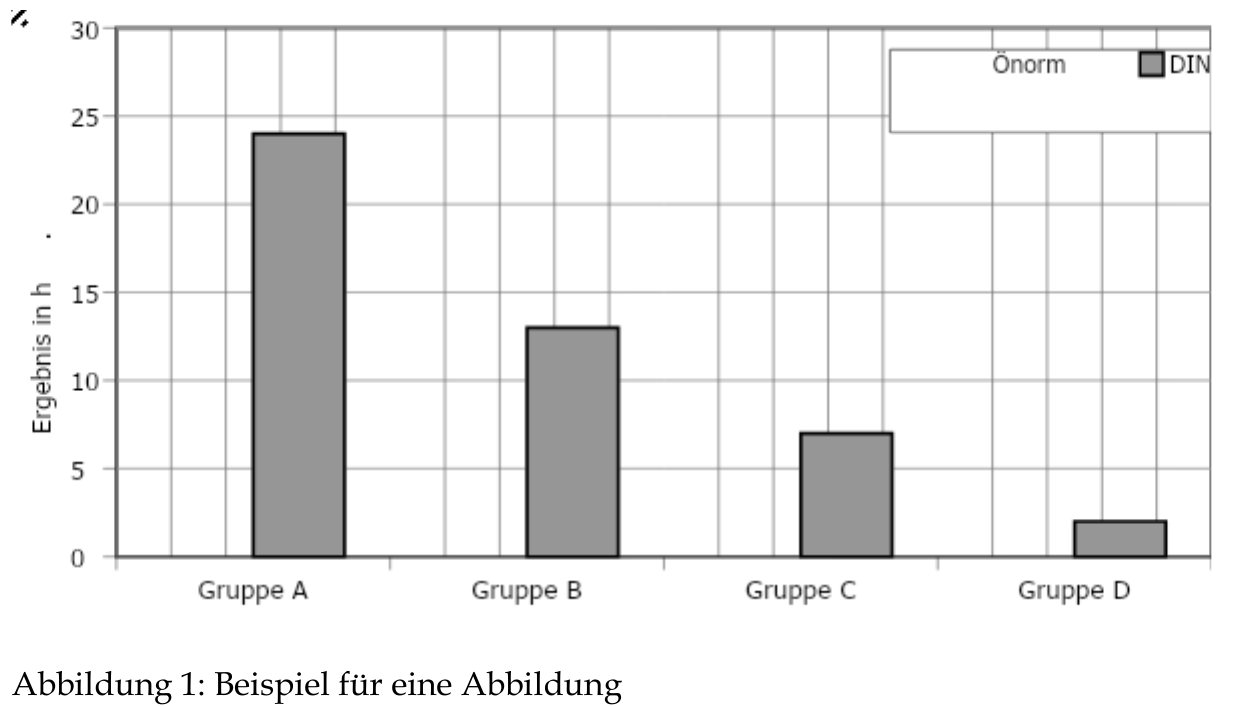
\includegraphics[width=0.7\linewidth]{figures/Word_Diagram}
%	\caption{Screenshot example from FHBgld word processor template}
%	\label{fig:worddiagram}
%\end{figure}
%\linebreak
%Mathematisch werden die Zusammenhänge wie im Figure \ref{fig:wordformel} beschrieben.
%\begin{figure}
%	\centering
%	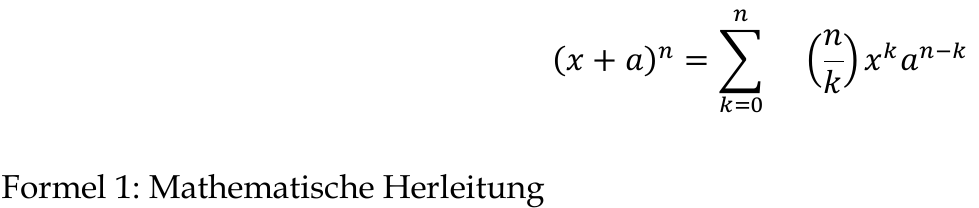
\includegraphics[width=0.7\linewidth]{figures/Word_Formel}
%	\caption{Screenshot example from FHBgld word processor template}
%	\label{fig:wordformel}
%\end{figure}
%
%\section{Tables and Images with \LaTeX}
%One of the great advantages of \LaTeX{} is that all it needs to know is
%the structure of a document, and then it will take care of the layout
%and presentation itself.  So, here we shall begin looking at how exactly
%you tell \LaTeX{} what it needs to know about your document.
%
%\subsection{Tables}
%In this sub-section, a simple table is inserted. To add reference to the table, see (cf. Table~\hyperref[tab:tableexample0]{\ref{tab:tableexample0}}):
%
%%A simple table.  The center environment is first set up, otherwise the
%%table is left aligned.  The tabular environment is what tells Latex
%%that the data within is data for the table.
%% https://en.wikibooks.org/wiki/LaTeX/Tables
%\begin{table}[htb]
%	\begin{tabular}{|b{7cm}|c|}
%		%The tabular environment is what tells Latex that the data within is
%		%data for the table.  The arguments say that there will be two
%		%columns, both left justified (indicated by the 'l', you could also
%		%have 'c' or 'r'.  The bars '|' indicate vertical lines throughout
%		%the table.
%		
%		\hline  % Print horizontal line
%		\fontsize{11pt}{12pt}\selectfont Command & Level \\ \hline  % Columns are delimited by '&'.  And
%		%rows are delimited by '\\'
%		\fontsize{10pt}{14pt}\selectfont Some sections to provide some examples: & \\
%		\texttt{\textbackslash part\{\emph{part}\}} & -1 \\
%		\texttt{\textbackslash chapter\{\emph{chapter}\}} & 0 \\
%		\texttt{\textbackslash section\{\emph{section}\}} & 1 \\
%		\texttt{\textbackslash subsection\{\emph{subsection}\}} & 2 \\
%		\texttt{\textbackslash subsubsection\{\emph{subsubsection}\}} & 3 \\
%		\texttt{\textbackslash paragraph\{\emph{paragraph}\}} & 4 \\
%		\texttt{\textbackslash subparagraph\{\emph{subparagraph}\}} & 5 \\
%		\hline
%		
%	\end{tabular}
%	\caption{some description of the table}
%	\label{tab:tableexample0}
%\end{table}
%
%\subsubsection{More tabular examples}
%
%First, a plain simple example for a FHBgld table, see table~\hyperref[tab:tab:tableexample1]{\ref{tab:tableexample1}}.
%
%\begin{table}[h]
%	\centering
%	\begin{tabular}{|b{1cm}|b{2cm}|b{3cm}|b{4cm}|}
%		\hline
%		\multicolumn{4}{|l|}{\fontsize{11pt}{12pt}\selectfont\noindent First line in 11pt fontsize } \\ \hline
%		1cm & 2cm & 3cm & 4cm \\ \hline
%		from & here on & the table & font size \\ \hline
%		will & be as & defined & in class, that is 10pt\footnote{yes, really!} \\ \hline
%		will & be as & defined & in class, that is 10pt\footnote{yes, really!} \\ \hline
%		will & be as & defined & in class, that is 10pt\footnote{yes, really!} \\ \hline
%		will & be as & defined & in class, that is 10pt\footnote{yes, really!} \\ \hline
%		will & be as & defined & in class, that is 10pt\footnote{yes, really!} \\ \hline
%	\end{tabular}
%	\caption{some description of the table}
%\label{tab:tableexample1}
%\end{table}
%
%Next, a table with nine columns, see table~\hyperref[tab:tableexample2]{\ref{tab:tableexample2}}.
%
%\begin{table}[h]
%	\centering
%	\begin{tabular}{|*{9}{l|}}
%		\hline
%		{\fontsize{11pt}{12pt}\selectfont This} & {\fontsize{11pt}{12pt}\selectfont table} & {\fontsize{11pt}{12pt}\selectfont has} & {\fontsize{11pt}{12pt}\selectfont way} & {\fontsize{11pt}{12pt}\selectfont too } & {\fontsize{11pt}{12pt}\selectfont many} & {\fontsize{11pt}{12pt}\selectfont columns}, & {\fontsize{11pt}{12pt}\selectfont does'nt} & {\fontsize{11pt}{12pt}\selectfont it?} \\ \hline
%		One & Two & Three & Four & Five & Six & Seven & Eight & Nine! \\ \hline
%		At & least & the & first & column & has & 11pt & font & size. \\ \hline
%	\end{tabular}
%	\caption{some description of the table}
%	\label{tab:tableexample2}
%\end{table}
%
%\subsection{Images}
%% Here is how to insert an image as a figure. There is a lot more you can do
%% when inserting images, check out: https://en.wikibooks.org/wiki/LaTeX/Importing_Graphics
%
%\begin{figure}[h]
%	\centering
%	
\includegraphics[width=0.3\textwidth]{figures/logo_nontransparent.jpg}
%	\caption{Image Example}
%	\label{fig:image_example}
%\end{figure}
%
%When an image is inserted, you can refer to it like this (cf. Figure~\hyperref[fig:image_example]{\ref{fig:image_example}}).
%
%\subsubsection{A Subsubsection}
%As one last example, this is how you can insert a sub-sub-section! Have fun
%writing your thesis with \LaTeX{}!
%
%\lipsum[2-3]
%\raggedbottom
%
%\pagebreak

%\chapter{Discussion and Interpretation}

%Results, Discussion and conclusions come here.

TODO

The overall goal of the thesis is to
provide a solution to the problem of release promotion in GitOps environments.
In this regard a prototype will be developed
and its functionality demonstrated in a proof-of-concept evaluation.
The goal for the prototype is to implement it as a modular extension to Kubernetes
and existing GitOps tooling.
By doing so, users can promote releases between multiple deployment environments
following the GitOps principles.
The main contribution of this thesis is a proof of concept for the developed prototype
which can be used as an extension to the GitOps toolkit within the CNCF.









\section{Learnings From The Prototype Implementation}

TODO

- ...

- User Feedback From Interview Partners








\section{Towards Standardized GitOps Promotions}

TODO






\section{Related Ideas And Approaches}

TODO






\section{?}
































%
%\section{Instruction included in the original FHBgld word processor template}
%Die Ergebnisse der Arbeit sind in übersichtlicher Form darzustellen Die gewählte Form der Darstellung ist vom gewählten Datenmaterial und den in der Einleitung gesetzten Zielen abhängig. Die Ergebnisse sind zu interpretieren und in Bezug zum Stand des Wissens zu diskutieren. Über die Beantwortung der Forschungsfrage und die daraus gezogenen Schlussfolgerungen schließt sich der Bogen zur Einleitung. 
%
%Wichtig ist die gedanklich klare Unterscheidung zwischen der Darstellung der Ergebnisse und der Interpretation/Bewertung der Ergebnisse. 
%
%\section{Code}
%If you want to show program code within your thesis you can use the \verb|\texttt{verbatim}| environment or for a more complex display take a look at \url{https://www.overleaf.com/learn/latex/Code_listing}
%
%\begin{verbatim}
%	Text enclosed inside \texttt{verbatim} environment 
%	is printed directly 
%	and all \LaTeX{} commands are ignored.
%\end{verbatim}
%
%\begin{lstlisting}[language=Python, caption=Python example]
%	import numpy as np
%	
%	def incmatrix(genl1,genl2):
%	m = len(genl1)
%	n = len(genl2)
%	M = None #to become the incidence matrix
%	VT = np.zeros((n*m,1), int)  #dummy variable
%	
%	#compute the bitwise xor matrix
%	M1 = bitxormatrix(genl1)
%	M2 = np.triu(bitxormatrix(genl2),1) 
%	
%	for i in range(m-1):
%	for j in range(i+1, m):
%	[r,c] = np.where(M2 == M1[i,j])
%	for k in range(len(r)):
%	VT[(i)*n + r[k]] = 1;
%	VT[(i)*n + c[k]] = 1;
%	VT[(j)*n + r[k]] = 1;
%	VT[(j)*n + c[k]] = 1;
%	
%	if M is None:
%	M = np.copy(VT)
%	else:
%	M = np.concatenate((M, VT), 1)
%	
%	VT = np.zeros((n*m,1), int)
%	
%	return M
%\end{lstlisting}

%\chapter{Future Work}
\label{future-work}

In this chapter,
further suggestions for future research on this topic and the developed prototype are presented.

In addition,
some interesting ideas that came out of this research are discussed,
and how they could be further researched in future work either by the researcher of this thesis or other researchers.



\section*{Further Research \& Development of the Prototype}

The proposed software prototype should be evaluated against its user experience,
in order to find out if users have difficulty doing the initial setup,
or any other troubles.
The use of the prototype could be observed in a case study or tested in a field experiment.
The prototype should be adapted in more iterations of the applied methodology process model.

The API, the custom resources, which the operator provides can be changed to fit the users needs.
Additional functionality which is required by users, can be added.
Since the operator works with any other GitOps tooling the users bring from their individual GitOps setup,
it can lack a bit of ease of use. The integration into other GitOps tooling like Argo or Flux
should be evaluated, and examined if such an integration is worth it, in order to provide better convenience.

The main goal is to extensively adapt for user requirements, in order to fit
many possible promotion processes.
The prototype should be further developed to enable the use in production by organizations or other projects.

\section*{Rolling Production Environments}

The term rolling production environments was coined by interview partner 1 during the interview.
It was discussed in section \ref{insights-related-ideas-approaches} earlier in this thesis.
The term represents a future idea of where promotions and rollouts of new releases could be heading to.
This approach steers in a somewhat other direction, than what this thesis researched.
Instead of having fixed testing environments or stages, which a new release needs to pass,
before being rolled out to the production environment,
this approach conversely foresees only the single environment,
which is actually used for production.

This approach builds upon the progressive delivery pattern,
which can be implemented with tools like Flagger or Argo Rollouts.
Instead of just doing progressive delivery of an application (i.e. Kubernetes deployment / container image),
the progressive delivery would be done on a whole environment (i.e. Kubernetes cluster).
This has the advantage of further limiting the chance of supporting services and applications
influencing the actual user-facing application in a bad way, i.e. breaking the service, making it unavailable for its users.
Each different supporting application constantly changes versions, and all these changes could potentially break some other dependency.
Some infrastructure components are sometimes even updated without a version history,
eliminating the possibility to roll back to a safe and working state.

One possible future work that could be done for evaluating this new approach,
could be to evaluate the costs and feasibility of this approach.
According to interview partner 1, tools like the Weave GitOps Terraform Controller
have made it a lot easier to achieve the idea of rolling production environments.
However since a whole production environment would be dynamically created with each new release,
this could introduce higher costs.
Especially in a cloud environment, where billing is done on-demand per minute used,
and where the costs can be an important factor for deciding between different architectures.

\section*{Overview of GitOps Repositories}

Discussed by interview partner 2 and presented in section \ref{insights-related-ideas-approaches}
is the idea and problem, that when a human is given a GitOps repository,
it is often difficult to understand how the setup is exactly structured,
what the environments are,
what the versions are,
and what applications and version are deployed where.
The overview that GitOps shall give,
with the single place to look and know what is your system's state,
is not as good as it is expected,
interview partner 2 mentioned.

As possible future research on this idea,
this problem statement could be evaluated with a survey research against GitOps users.
In addition, especially if the survey's results speak for this statement,
a software tool could be developed,
which can recognize filesystem structures and plain text configuration files,
which represent the desired state.
This tool would have have knowledge of the different configuration management tools like Kustomize or Helm.
It would probably be beneficial to have a visual representation in the form of a dashboard.

Such a visual representation is already provided by ArgoCD for example,
however it will only show the configured data in the dashboard.
Any files, which are not yet added to the specific ArgoCD instance,
can only be viewed by having a look into the Git repository's filesystem manually.




\section*{Towards Standardized GitOps Promotions}

There is no standard way of doing promotions with the GitOps approach.
Sometimes a container image tag is changed in some place or places,
other times multiple files are copied over to another place (like the promotion process proposed with the prototype in this thesis),
and other times a promotion consists of multiple processes spanning over different domains.
This differs for each individual setup for distinctive organizations.

In order to get a better understanding of what the requirements are for different organizations,
and how they imagine a solution, and solved their individual use case,
it would be of use to survey a wide range and variety of organizations which adopted or want to adopt the GitOps approach.
For open-source tooling it is beneficial to strive for functionality that can be used by everyone,
instead of providing tailored tooling which may only work for a single setup at a particular organization.

















\chapter{Conclusion}
\label{conclusion}

%In einer Conclusio wird keine neue Information präsentiert, sondern das bereits gesagte nochmal zusammenfassend wiedergegeben. Du möchtest hier dem Leser die wichtigsten Key Points deiner Arbeit mitgeben, so dass er sich ewig dran erinnernt.
%
%In welchem Forschungsfeld sind wir nochmal und was ist das eigentlich Problem dort?
%
%Welcher Lösungsvorschlag wurde präsentiert, um dieses Problem zu lösen und welche Methodik wird eingesetzt, um das zu schaffen?
%
%Ausblick...wenn wir das dann geschafft haben, was können wir dann mehr, was wir heute nicht können?
%
%Future Work -> welche neuen Forschungsfelder eröffnen sich dann, wo können wir ab dann weitermachen?


In this final chapter,
no new information is presented,
but what has already been said is summarized again.
The most important key points of the thesis are highlighted,
in order for the reader to easily consume.

\section*{Problem}

The increasing adoption of a DevOps culture in organizations to develop applications and services quickly,
and reduce friction between people, communications and technical processes,
to ultimately decrease the time to market for new product releases,
has brought forward a new practice called GitOps.

One of the unresolved problems of the GitOps practice is
the process of promoting releases between multiple deployment environments.
Current tools in the ecosystem do not provide an integrated solution for this process.
Users are therefore inclined to build workflows which are constrained to specific
Git providers, GitOps engines,
CI/CD system, and configuration/templating tools. This can lead to tightly coupled setups,
and vendor lock-in.

In this research,
the given problem was addressed by designing uniform, standardised models for
defining GitOps-native deployment environments and promotion processes.
These models were implemented in a prototype as custom resources and controllers with the
operator pattern, as a Kubernetes extension.
This developed software artifact allows users to define abstract representations
of their environments, and how they want releases to be promoted between them.

\section*{Research Question}

The overall goal of the thesis was to provide a solution to the problem of
release promotion in GitOps environments.
Therefore this overarching research question was defined:
\textbf{\ref{RQ1}};
with the following sub research questions:
\textbf{\ref{RQ1.1}}
\textbf{\ref{RQ1.2}}

\section*{Methodology}

In order to help with recognition and legitimization of the conducted research,
the methodology for conducting design science research in information systems
\autocite{designScienceResearchMethodologyForInformationSystemsResearch}
was applied, which consists of six activities.
%\nameref{methodology:activity1},
%\nameref{methodology:activity2},
%\nameref{methodology:activity3},
%\nameref{methodology:activity4},
%\nameref{methodology:activity5},
%\nameref{methodology:activity6}.
In activity 1,
the research problem of
release promotion with GitOps
was defined.
This was done primarily with the help of practicing professionals in the GitOps field,
which were interviewed.
In activity 2,
research objectives were inferred from the problem definition in activity 1.
Each objective maps to a distinct item from the problem specification,
which helped with later evaluation in activity 5.
In activity 3,
solutions for the previously defined objectives were designed and developed
by means of producing an artifact, namely the GitOps Promotions Operator prototype.
In activity 4,
the in-context use of the artifact was demonstrated in a proof of concept.
In activity 5,
the implementation of the artifact,
and how well it supports a solution to the problem,
was evaluated.
In activity 6, as a final step,
the whole conducted research was communicated by means of
publishing it as a master thesis.

\section*{Related Work}

Prior research on the concrete problem is focused on presenting
best practices and suggestions
which users need to manually implement themselves.
In addition it is suggested to let an external CI/CD system handle the promotion process.
Conversely, this thesis brought forward
abstract models of environments and promotion processes,
which are implemented in the proposed prototype operator,
as Kubernetes custom resources and controllers, with the operator framework.
The prototype will assess the feasibility of
defining deployment environments and promotion processes declaratively,
following the GitOps principles.

\section*{Theoretical Background}

The theoretical background on the topic was brought forward to the user,
in order to aid comprehension of the material within the thesis.
General definitions of terms,
fundamentals of GitOps along related tooling and components were presented.
DevOps and internal developer platforms were mentioned.
It was explained, how many times the term GitOps is misunderstood,
and that GitOps is actually defined in the OpenGitOps project.
It was shown how GitOps changes the architecture and process of Continuous Deployment,
and how the promotion of releases is achieved without and with the GitOps approach.
Emerging patterns like progressive delivery,
as well as the concept behind short-living environments were described.
The power of Kubernetes as a cloud native platform and its use cases beyond container orchestration were presented.
Finally it was shown how the declarative representations of GitOps environments are typically modelled currently.

\section*{Interviews}

For the problem identification and motivation of the main topic of this thesis,
%namely the promotion of releases in GitOps environments,
interviews with practicing professionals, who are working in the GitOps field, were conducted.
Several problems were identified,
and defined along with their respective research objectives.
\textbf{\nameref{problem1}},
relates to a frequent issue with currently available tooling in the GitOps ecosystem. 
Often times solely container image version tags are the focus with current tools when promoting
new versions or releases.
%It was discussed, that this is insufficient for some use cases.
Because it is sometimes required to handle all sorts of resources, not just the version tag of a container image,
an according research objective was defined.
%Especially when not using containerization technologies for runtime, this is an important problem to handle.
%In order to be able to provide a solution to this problem with a comprehensible approach,
%a solution objective was inferred and its requirements defined.
\textbf{\nameref{objective1}},
defines a qualitative description of how the respective problem is supposed to be solved
by the developed artifact. The main idea is to offer the capability to promote arbitrary resources,
meaning any type of resource, instead of solely the container image version.
%The technical implementation in the proposed prototype foresees the functionality for
%promoting a list of filesystem paths inside the Git repository of the desired state to other environments.
%In addition these arbitrary resources should be able to be assigned a descriptive name,
%in order to identify the promotion subjects more easily.
\textbf{\nameref{problem2}},
states the fact, that it is not a straight-forward process of how the order of promotion
through multiple GitOps environments can be setup.
%When adhering to the principles of GitOps
%and sticking with the asynchronous deployment process (described in the
%\nameref{theoretical-background} chapter)
%there is no streamlined approach or tooling, that automates this, while still sticking to the asynchronous process.
\textbf{\nameref{objective2}},
defines the requirements for the proposed prototype,
in regards to the according problem of having a certain order of promotion through environments or stages.
The objective describes the capability for defining a certain order of environments, in which releases traverse through.
In addition, this solution objective opens up the possibility to setup promotion in stages, in which
certain environments must be deployed to first, before the release can deploy to other specified environments.
\textbf{\nameref{problem3}},
relates to the problem that when wanting to promote a new release from environment one to another environment,
it is not easily achievable with the available tools to specify certain dependencies, like other workloads or
microservices in the same or another environment, or altogether dependencies from external sources.
This is especially desirable for evaluating test results or other metrics, before triggering the promotion.
\textbf{\nameref{objective3}},
describes how the respective problem of being able to specify dependencies for a promotion,
could be solved in the proposed prototype. While the minimum dependency is the successful deployment
of the workload of a release,
it may also be desirable to specify other resources or workloads which need to be in a certain state,
before triggering a promotion.
\textbf{\nameref{problem4}},
draws attention to the common problem of being dependent on single tools and providers.
The more complex the Continuous Delivery is setup for a particular project,
the more difficult it is to de-couple or switch providers for certain components.
%Furthermore, since many tools in the GitOps ecosystem are not very mature in their development and adoption,
%it is of use that components are loosely coupled and can be exchanged with alternatives in the future.
\textbf{\nameref{objective4}},
defines the requirements of how a vendor-neutral and tool-agnostic prototype can be implemented.
%The main components which are desirable to support all alternatives,
%for being able to switch between them,
%are the Git providers (e.g. GitHub, GitLab),
%the GitOps engines (e.g. Argo, Flux),
%the configuration/templating tools (e.g. Kustomize, Helm).
Additionally,
related ideas and approaches were discussed by the interview partners.
These points were not directly considered for the conducted design science in the prototype,
however they were discussed later.

\section*{Prototype}

The proposed prototype was presented.
The asynchronous nature of GitOps deployments, and where
the operator prototype fits within this architecture was described.
Abstract models for the environment and promotion custom resources as well as their prototype
design as declarative Kubernetes custom resources was described.
The implementation of these custom resources was shown in the form of mockups
of Kubernetes custom resources in the YAML format.
Alternative mockup designs were shown as a way to draw attention to the fact
that the actual design of the API specification is not cast in stone.
Moreover, the API specification should be tested with users of it,
and should be adapted for usability and ease of use.
The translation of the API specification in YAML format into Go types was described,
and finally the implemented controller logic of both the environment, as well as
the promotion controller was presented.
The developed artifact of the prototype operator was
demonstrated in the context of a proof-of-concept use case.
The demonstration of the prototype's functionality was then evaluated against
%the research objectives defined in
%\ref{interviews:definitionSolutionObjectives} \nameref{interviews:definitionSolutionObjectives}.
the research objectives.

\section*{Evaluation \& Results}

The results of the conducted research were presented, primarily by means of
presenting and describing the designed and developed operator prototype, and the learning
from the prototyping process.
In addition, the interviewed working professionals gave several interesting insights into the problem
statement from their point of view.
The results of the research were evaluated on how they provide a solution to the research problem.
The implemented functionality of the prototype was evaluated against the research objectives.
This was done by comparing the qualitative descriptions of the objectives with the actual observed results
in the demonstration of the prototype in the proof of concept.
% ?? feedback for the prototype from the working professionals??
For the research question RQ 1.1,
a possible solution was presented by means of
describing the design of a prototype of a Kubernetes operator for handling GitOps promotions.
For research question RQ 1.2,
a possible implementation of the abstract models was presented, in the form of
declarative custom resources, which extend the Kubernetes API.
The overarching research question 1 is the combination of the sub research questions.
The thesis proposes one possible way of how the research problem can be addressed,
namely the promotion of releases in GitOps environments can be designed.
This concrete research does not try to propose a definitive answer or solution to the research question.

\section*{Discussion \& Interpretation}

The results, learnings, and evaluations of the research were discussed and interpreted.
The meanings behind the specific results are brought forward in more detail.
Moreover, interpretations and implications of the results and evaluations were presented.
Learnings from implementing the prototype were presented, namely
ideas about the user experience, security considerations, the use at scale, abstractions and modularity.
Alternative approaches for promoting releases were presented, as mentioned by interview partner 1.
%
%The main idea of this approach is that long-living environments are not necessary,
%and the resiliency should rather be created by doing progressive delivery,
%not just for the user-facing application or service,
%but for the whole infrastructure stack below.
%This has the purpose of further increasing the immutability and resiliency of a service.
%Since the amount of supporting and infrastructure services and dependencies are increasing with Kubernetes,
%and each having a version and constantly new releases, and the possibility of breaking the actual important
%service that is user-facing.
%
%When following this approach, the end goal is to create a complete copy of the production environment,
%and then do progressive delivery on that.
%Once the release is marked as good, the old production environment can safely be destroyed.
%With the GitOps pattern, and the application and infrastructure being stored in Git,
%this has become increasingly more possible.
%Also tools like the Weave GitOps Terraform Controller have contributed to the enablement of this new approach. 
%
%While, with this approach, the need for long-living environments decreases,
%whole copies of production environments will still need to be created.
%This means there is no guarantee that the cost will decrease.
%Advanced tactics like auto-scaling will need to be implemented, in order to
%keep costs low of potentially high numbers of dynamically created environments.
%

\section*{Future Work}

Further suggestions and point of references for future research on this topic
and the developed prototype were presented.
These included
further research and development of the proposed prototype,
which is about testing its user experience, evaluating integration with
other GitOps tools. Generally the aim is to enhance the prototype
to make it mature for production use.
The idea of rolling production environments by interview partner 1 was discussed.
It describes a somewhat different approach for promotions in GitOps,
where less environments are needed, but for each new release the 
production environment is re-created with the new versions, and
progressive delivery is done not only on an application level, but on the whole
infrastructure stack together with the end user application or service on top.
This is to further improve immutability and versioning to increase resiliency.
The idea of the problem with the overview of GitOps repositories by interview partner 2
was discussed.
It is about the somewhat missing feature of an quick and easy to understand overview over a GitOps repository.
Depending on the used configuration/templating tool, a setup looks different.
Deployment environments can be represented, however it is not possible for the user
to know what the target environment is, or where the GitOps definition is deployed to in general.
Moreover it was discussed that it would make sense for future work
to research a wide range and variety of organizations and do a survey on
their requirements, their issues and how they imagine a solution.
An initiative towards standardized GitOps promotions should be made,
because for open-source tooling the aim should be to strive for functionality
that can be used by everyone,
instead of providing tailored tooling which may only be beneficial for specific use cases
and organizations.



























%The currently available GitOps tools
%do not provide an integrated solution to
%the problem of promoting releases between environments.
%This thesis aims at addressing the given problem.
%This is achieved by
%clearly defining the problem in distinct items,
%from which research objectives are then inferred.
%Following in designing and developing abstract models for
%environments and promotion processes;
%which are implemented in the produced artifact "release promotion operator".
%The artifact is demonstrated in a prototype serving as a proof-of-concept.
%Finally the research is evaluated by means of
%comparing the artifact's functionality with the solution objectives.
%
%The developed "release promotion operator" prototype should serve as
%a modular extension to Kubernetes and existing GitOps tooling within the CNCF.
%It should provide a more streamlined and GitOps-native approach
%to the process of release promotion.
%For subsequent research projects the use of the prototype could
%be observed in a case study or tested in a field experiment,
%and adapted in another iteration of the applied methodology process model.
%The main goal for future work is the extensive adaption of the prototype
%to enable use in production by organizations or other projects.






























%
%\section{Instruction included in the original FHBgld word processor template}
%Die Zusammenfassung stellt die gesamte Arbeit – von der Einleitung bis zu den Ergebnissen - in Kurzform dar. Länge maximal 1,5 - 2 Seiten. 
%
%\section{Algorithms}
%
%If you want to show algorithms in your Thesis take a look at the \url{https://www.overleaf.com/learn/latex/algorithms} page. The \verb|algorithm2e| package is already included in the template. You can list algorithms in the same way as you can list Tables and Figures.
%
%\begin{algorithm}[H]
%	\KwData{this text}
%	\KwResult{how to write algorithm with \LaTeX2e }
%	initialization\;
%	\While{not at end of this document}{
%		read current\;
%		\eIf{understand}{
%			go to next section\;
%			current section becomes this one\;
%		}{
%			go back to the beginning of current section\;
%		}
%	}
%	\caption{How to write algorithms}
%\end{algorithm}
%%\cleardoublepage{}
%
%\section{Acronyms and Glossary.}
%
%if you want to use Acronyms or a Glossary check the page here: \url{https://www.overleaf.com/learn/latex/glossaries}
%
%The \Gls{latex} typesetting markup language is specially suitable 
%for documents that include \gls{maths}. are 
%rendered properly an easily once one gets used to the commands.
%
%Given a set of numbers, there are elementary methods to compute 
%its \glsxtrlong{gcd}, which is abbreviated \glsxtrshort{gcd}. This 
%process is similar to that used for the \glsxtrfull{lcm}.
%
%\section{Macros}
%
%You can also add useful packages or macros into the \verb|packages_macros.tex| file to add them to the project.
%The packages for algorithms, code or the glossary have already been added there.
%
%\subsection{FixMe}
%Another example, the \verb|FixMe| package, is added as well. It allows you or your supervisor to add Meta comments to the document. These comments only appear if you set the draft mode in the \verb|main.tex| file. If you remove or comment the activation of the draft mode you can see your final thesis without comments.
\chapter{Einleitung und Problemhintergrund}

Adaptives Scheduling von Arbeitslasten in heterogenen Cluster-Umgebungen, basierend auf Energieeffizienz

Forschungsfeld (Universum), 5-7 Sätze

Was ist denn das überhaupt

Idee 1

Idee 2

Idee 3

Idee xy

Zusammenfassung

Problemstellung, 5-7 Sätze

Forschungsvorhaben, 5-7 Sätze

Ausblick, 3-5 Sätze


\titleformat{\chapter}{\normalfont\Large}{\thechapter}{20pt}{\normalfont\Large}
\printbibliography[title=\thesisBookLiteratureLabel]
\end{document}


% if not used with overleaf add data input here
%% if not using overleaf - data is needed separately
\newcommand{\typeOfWork}{Master Thesis}
\newcommand{\titleToObtain}{Master of Science in Engineering}
\newcommand{\studyProgram}{Master Program Cloud Computing Engineering}
\newcommand{\yourNameInclTitle}{Akademische(r) Grad(e)  Vorname Zuname}
\newcommand{\yourMatNumber}{12345678}
\newcommand{\supervisorNameInclTitle}{Akademische(r) Grad(e)  Vorname Zuname}
\newcommand{\departmentName}{Department Informationstechnologie und Informationsmanagement}
\newcommand{\yourThesisTitle}{Please enter your Thesis Title here, up to 70 characters. If necessary, adapt spaces in FHBgld\_Thesis.}
\newcommand{\thesisDate}{March \ordinalnum{17} 2021}
\newcommand{\universityCityCountry}{FH-Burgenland, Eisenstadt, Österreich}
\newcommand{\thesisBookLiteratureLabel}{Literaturverzeichnis}
\hypersetup{
    pdftitle={\yourThesisTitle},
    pdfsubject={\typeOfWork},
    pdfauthor={\yourNameInclTitle},
    breaklinks, % permits line breaks for long links
    bookmarksnumbered,        % ... and include section numbers
    linktocpage,        % "make page number, not text, be link on TOC ..."
    colorlinks,            % yes ...
    linkcolor=black,        % normal internal links;
    anchorcolor=black,   
    citecolor=black,
    urlcolor=blue,        % quite common
    pdfstartview={Fit},        % "Fit" fits the page to the window
    pdfpagemode=UseOutlines,    % open bookmarks in Acrobat
    plainpages=false      % avoids duplicate page number problem
}

\begin{document}
\pagestyle{empty}
\pagenumbering{gobble}


\begin{flushleft}
    \LARGE{\yourThesisTitle}
\end{flushleft}
\subsectionfont{\fontsize{13}{16}\normalfont}
\titlespacing\subsection{0pt}{0ex}{0ex}
\subsection*{\yourNameInclTitle}
\vspace{-0.5em}
\noindent{\textit{\universityCityCountry}}

% define header appearance
\titleformat{\chapter}{\normalfont\large}{\thechapter}{20pt}{\normalfont\large\MakeUppercase}
\chapterfont{\fontsize{13}{16}\normalfont\MakeUppercase}
\titlespacing\chapter{0pt}{2ex}{2ex}
\sectionfont{\fontsize{13}{16}\normalfont}
\titlespacing\section{0pt}{0ex}{0ex}
\subsectionfont{\fontsize{13}{16}\normalfont}
\titlespacing\subsection{0pt}{0ex}{0ex}
\subsubsectionfont{\fontsize{13}{16}\normalfont}
\titlespacing\subsection{0pt}{0ex}{0ex}
% numbering subsubsections
\setcounter{secnumdepth}{5}

% do not start chapter on new page
\makeatletter
\patchcmd{\chapter}{\clearpage}{\leavevmode\flushleft}{}{}
\makeatother

\vspace{5em}
\begin{abstract}
    % TODO:  abstract!

\noindent
Aus den Prinzipien von DevOps entstand GitOps,
als eine Sammlung von Prinzipien und Best Practices
für die Operation von Softwaresystemen. Im Zentrum
bzw. der Quelle - als einzig wahre Quelle (Single Source of Truth) -
steht dabei das Git-Repository bzw. ein Revisions-Kontrollsystem.
Der Zustand des zu verwaltenden Systems wird
vollständig deklarativ als Code definiert. Ein GitOps-Controller
kümmert sich um den kontinuierlichen Abgleich zwischen dem
definierten Ziel-Zustand und dem tatsächlichen Systemzustand.
Die Promotion neuer Software-Releases zwischen mehreren Umgebungen
zeigt sich als derzeit offenes Problem.
Es fehlen einheitliche Standardpraktiken, sowie nötige Tools in der Open-Source-Community.
Diese Arbeit hat als Ziel,
die Promotion von Releases in GitOps-Umgebungen
zu addressieren.
Es sollen abstrakte Modelle von Deployment-Umgebungen
sowie Promotion-Workflows definiert werden.
Aufbauend auf den zuvor definierten Modellen soll eine
standardisierte Lösung zur Promotion von Releases
nach den GitOps-Prinzipien implementiert,
und den bestehenden Lösungen gegenübergestellt werden.

%Der Leser der Kurzfassung soll verstehen, welche Problemstellung / Fragestellung durch die vorliegende Arbeit bearbeitet wird und welche Erkenntnisse und Ergebnisse vorliegen.



\end{abstract}
\vspace{2em}
%
\chapter{Introduction}

TODO

\section{Problem Statement}

% 1. Absatz: Beschreibe uns das Forschungsfeld in dem du dich befindest (DevOps / GitOps)

%\noindent
Increasingly more organizations are adopting 
a DevOps culture to develop new applications and services at high velocity. 
After all, a culture that encourages shared responsibility, transparency and rapid feedback, 
helps to narrow the gaps between teams and thus accelerate the development process.
In order to
reduce friction between engineering teams who are involved in the software development lifecycle (SDLC),
a new practice called GitOps has emerged.
It allows developers who are already familiar with the revision control system Git,
to easily deploy their applications to target environments in a self-service model.
System administrators and operators can also manage IT infrastructure
purely by interfacing with declarative state definitions stored in Git.
%GitOps is a set of principles for operating and managing software systems.
%These principles are derived from modern software operations, but also have their roots 
%in existing and widely adopted best practices. 
\bigskip

% 2. Absatz: Beschreib uns das Problem bzw. die Challenge in diesem Forschungsfeld (Was ist die Problemstellung, die es zu bearbeiten gilt)

% why is it important to solve the problem?

\noindent
GitOps as a practice for releasing software has many advantages,
but like other solutions, GitOps also has some shortcomings.
One of the unresolved problems is
the process of promoting releases between multiple deployment environments (illustrated in Figure \ref{fig:releasePromotionProcess}).

\begin{figure}[h]
	\centering
	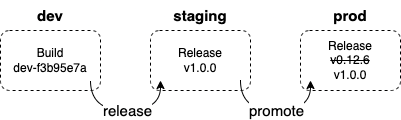
\includegraphics[width=.55\linewidth]{figures/release-promotion.drawio.png}
	\caption{release promotion process.
		%		(\citeauthor{ref}, \citeyear{ref}).
	}
	\label{fig:releasePromotionProcess}	
\end{figure}

\noindent
Current GitOps tools do not provide an integrated solution for this process,
nor do they provide any sort of abstraction for defining environments.
Users currently need to rely on separation of duties
on a file and folder level within the Git repository,
for modeling different environments.
Promotions are often achieved via hard-coded file copy operations,
which is done manually or by a
Continuous Integration (CI)/Continuous Delivery (CD) system.
Due to the nature of Git, a certain flow of promotion can not currently be enforced
(e.g. QA --> Staging --> Production).
Furthermore, for each configuration or templating tool which is used
(e.g. kustomize, helm, jsonnet, etc.),
the modeling of different deployment environments, as well as the
process of promotion, is unique.
This results in the process of promoting releases with GitOps
not being a streamlined task.
Clear guidelines and best practices,
as well as tools which implement them,
are missing in the GitOps ecosystem.
\bigskip

% 3. Absatz: Was schlägst du vor, wie man die Problemstellung bearbeiten könnte? Beschreibe uns deinen Lösugnsvorschlag dieser Arbeit, wie man das Problem bearbeiten könnte

\noindent
%
The given problem could be addressed by
providing standardised models 
for defining deployment environments and promotion processes.
%
An application programming interface (API) extension for Kubernetes
could provide custom resource definitions for these models.
%
This would allow users to define abstract representations of
their environments,
and how they want releases to be promoted between them.
%
Additional logic could be introduced into the promotion process,
like specifying a rule which ensures that new releases must first pass
certain environments or other objectives before being promoted to production.
%
The abstraction would also enable transparent replacement of the
configuration or templating tool,
while keeping the desired state definition intact.
%
Following the principles of GitOps,
an operator would ensure the continuous reconciliation
between the desired and the actual state of the resources.
\bigskip

% 4. Absatz: gib uns einen Ausblick (Paint the Big Picture) wie deine Lösung mit dem großen Ganzen zusammenhängt

\noindent
%
The proposed solution of the problem should
present a possible way of defining environments and promotion processes abstractly,
onto which future work could build upon.
%
Additionally the solution should
provide a protoype of a toolkit,
which could serve as an optional component
in addition to existing tooling within the Cloud Native Computing Foundation (CNCF).
%
Solving the problem of release promotion natively within the GitOps toolkit,
would make the adoption of GitOps more appealing,
especially for organisations, which have the need for many different environments.
%
As a result
this could generally accelerate the widespread use of GitOps
and thus enable more organisations to develop higher quality software.
%








\section{Research Questions}
\label{introduction:research-question}


% TODO: goal of this reasearch is ...
%The goal of this thesis is to
%address the problem of promoting releases between different environments in GitOps.
%\bigskip
%
%\noindent
Large organizations in particular typically have many
non-production and production environments
such as:
Development (Dev),
Quality Assurance (QA),
Staging-US,
Staging-EU,
Production-US,
Production-EU.
Usually new releases are automatically deployed to an environment,
such as QA, 
by a CI/CD system.
Now the task is to promote
new changes, which are brought about by a new release,
into subsequent or other environments.
Current GitOps tools do not have a simple answer to
the question about what is the right approach for the process of promotion.
\bigskip

%\noindent
%In particular, this thesis aims to explore
%existing strategies for the solution of the problem
%with existing tools.
%Furthermore, a prototype of a newly proposed strategy will be developed.
%Subsequently, the prototype will be tested in a laboratory experiment
%and compared to currently existing strategies.
%\bigskip

\noindent
To achieve the goal of the thesis, the following research questions (RQ) were identified:

\begin{itemize}
	\item RQ 1: How can the promotion of releases in GitOps environments be designed?
	\begin{itemize}
		\item RQ 1.1: What possibilities do existing tools offer for the promotion of releases with multiple deployment environments?
		\item RQ 1.2: How can deployment environments, as well as promotion processes be modeled abstractly?
		\item RQ 1.3: How can the abstract models be used to implement a standardized solution for promoting releases?
	\end{itemize}
\end{itemize}

% ensure bullet points do not span over page break on final PDF export






\section{Research Methodology}
\label{introduction:research-methodology}







\section{Thesis Structure}
\label{introduction:thesis-structure}








%Welcome to the \LaTeX{} template prepared for the Computer Science department at the university of applied sciences of Burgenland\footnote{\url{https://www.fh-burgenland.at/en/information-technology/about-the-department/}}. 
%
%Introduction, Problem, Objective, Demarcation, Question, Method, and a description of the overall structure should go into this chapter.


%
%\section{Instruction included in the original FHBgld word processor template}
%\subsection{Problem stating[!]}
%In der Problemstellung erfolgt eine Hinführung zum Thema aus dem globalen
%Zusammenhang heraus betrachtet: Warum es wichtig ist, sich mit dem konkreten
%Thema zu beschäftigen bzw. welche Bedeutung hat dieses Thema zum Beispiel für die
%Wirtschaft, Gesellschaft und Umwelt.
%\subsection{Research question and added value}
%Hier werden die konkrete(n)wissenschaftliche(n) Fragestellung(en) klar angeführt.
%Neben dem inhaltlichen Ziel der Arbeit wird fallweise auch angegeben, wie
%vorgegangen wird, um die Fragestellung zu bearbeiten (z.B. mit einem Online-
%Fragebogen). Auch die Zielgruppe der Arbeit und der für die Zielgruppe angestrebte
%Nutzen kann an dieser Stelle angeführt werden.
%Anmerkung:
%Die Erfahrung zeigt, dass es hilfreich ist, das erste Einleitungskapitel an die Betreuerin
%/ an den Betreuer zu schicken und Feedback dazu zu erhalten.
%Bitte auch darauf achten, dass alle Absatz-Abstände gleich groß sind.
%Jedes Kapitel sollte mit einem Satz beginnen und einem Satz enden und ca. mind. 1⁄2
%A4-Seite umfassen.
%
%\section{Using the \LaTeX{} template}
%
%Everything in the template revolves around the\verb|main.tex| file. Here all the other files are put together to create the thesis.
%There are three different sections to consider: 
%\begin{itemize}
%	\item Front Matter,
%	\item Chapters, and
%	\item Back Matter.
%\end{itemize}
%Each section has a folder where you can put the different parts of your thesis. In the Front Matter section you should put everything that comes before your first chapter of the thesis. Respectively, in the Back Matter section you put everything that comes after your last chapter. And finally all the chapters are put into the Chapters folder. You can put things like abstract, summaries, etc... wherever they suit your thesis. In the end it really only matters how you add them into your \verb|main.tex| file. With the \verb|\input{}| command you can add the parts if they should appear in your thesis, the order within the \verb|main.tex| also determines the order in the final pdf.
%
%\subsection{Title-page}
%The Layout of the Title-page is in the \verb|FHBgld_Thesis.cls|, normally it remains unchanged. You can use all the commands as seen in the \verb|Titlepage.tex|. 
%
%The template and also the titlepage is based on the scrbook class. So if you want to use a different class without changing the title page in the \verb|FHBgld_Thesis.cls|, it is recommended creating the title page separately and then include the compiled pdf file here, using the 
%\verb|\includepdf{<filename>}| from the \verb|pdfpages| package. Alternatively, you may use the word template for the title- page and add it using this package. In that way you can avoid any differences to the original title page template. The word templates can be found here:
%\begin{enumerate}
%	\item \url{https://moodle.fh-burgenland.at/pluginfile.php/34046/mod_folder/content/0/03_Vorlage_zur_Erstellung_wissenschaftlicher_Arbeiten\%20V2.8.docx?forcedownload=1}
%	\item \url{https://moodle.fh-burgenland.at/pluginfile.php/34046/mod_folder/content/0/03_Vorlage_zur_Erstellung_wissenschaftlicher_Arbeiten\%20V2.8\%20eng.docx?forcedownload=1}
%\end{enumerate}
%
%If you use the \verb|includepdf| package make sure that the pdf still has the correct metadata afterwards.
%
%\subsection{Citing}
%As per requirement of the FH Burgenland, the template class is configured for APA\footnote{\url{https://ctan.org/pkg/biblatex-apa?lang=en}} style: \verb|[natbib=true, backend=biber, style=apa, sorting=nty]|. It uses Biblatex and the Biber backend. The location of the bibliography file is defined in the \verb|main.tex|. Citation xamples:
%\begin{itemize}
%	\item \verb|\parencite{bibid}| provides \parencite{lamport94}
%	\item \verb|\parencite[p. 123ff]{bibid}| provides \parencite[p. 123ff]{lamport94}
%	\item \verb|\parencite{lamport94,talbot2013using}| provides \parencite{lamport94,talbot2013using}
%\end{itemize}
%
%\subsection{Temporary packages and settings}
%Some packages and settings are included to make creating your thesis easier, e.g. FixMe.
%Before building your final PDF, those should be removed. Use \verb|grep -r RMF *| in the root folder of the template to find the packages and settings that should be removed.
%
%\section{Creating the pdf}
%To create a proper pdf file of your thesis there are some things to consider
%
%\subsection{PDF build}
%The script \verb|build.sh| is provided to compile the thesis in four steps:
%\begin{enumerate}
%	\item pdflatex main.tex
%	\item biber main
%	\item bib2gls main
%	\item pdflatex main.tex
%\end{enumerate}
%\verb+bib2gls+ is used to prepare the indexes for glossaries and acronyms. Both are edited in \verb|defns.bib|, therefore, Jabref can be used to manage entries. 
%
%In case you already have your definitions in \LaTeX{} format, such as
%\begin{itemize}
%	\item \verb|\newacronym{gcd}{GCD}{Greatest Common Divisor}}|, or
%	\item \verb|\newglossaryentry{latex}{name=latex,description={Is a mark up language specially suited for scientific documents}}|
%\end{itemize}
%use \verb|convertgls2bib defns.tex defns.bib| to convert from \LaTeX{} to Bibtex.
%
%\subsection{Embed all fonts in pdf}
%Please make sure that you embed all fonts in your pdf. Also make sure all the fonts of any figures that were used in the document are embedded. 
%If you don't use any pdf figures, pdfLaTeX should embed all fonts automatically.
%
%\subsubsection{Linux}
%On Linux you can use the command \begin{verbatim}
%	pdffonts my_file.pdf
%\end{verbatim}
%to check if the fonts are embbeded. Check if all the fonts listed have a "yes" in the "emb" column. 
%\begin{verbatim}
%name                                 type              encoding         emb sub uni 
%------------------------------------ ----------------- ---------------- --- --- --- 
%BXJBCJ+NimbusSanL-Bold               Type 1            Custom           yes yes no     
%HEMYJL+NimbusSanL-Regu               Type 1            Custom           yes yes no     
%OOJWDR+SFRM1000                      Type 1            Custom           yes yes no      
%OHLNOC+SFRM0900                      Type 1            Custom           yes yes no   
%...
%\end{verbatim}
%For more information see 
%
%\url{https://www.karlrupp.net/2016/01/embed-all-fonts-in-pdfs-latex-pdflatex/}
%\subsubsection{Windows}
%On Windows using the Adobe Acrobat Reader the fonts can be found at
%\begin{verbatim}
%	File > Properties > Fonts
%\end{verbatim}
%For more information please consult
%\begin{enumerate}
%	\item \url{https://helpx.adobe.com/acrobat/using/pdf-fonts.html}
%	
%	\item \url{https://www.overleaf.com/learn/latex/Questions/My_submission_was_rejected_by_the_journal_because_%22Font_XYZ_is_not_embedded%22._What_can_I_do%3F} 
%	\end{enumerate}
%	
%	%\subsection{Making a PDF/A-1 compatible pdf}
%	\subsection{Making a PDF}
%
%	
%	\subsubsection{validation}
%	To validate the produced PDF, you can either use the Preflight tool included in Adobe Acrobat Pro or a free online version. E.g. \url{https://www.pdf-online.com/osa/validate.aspx}.
%	Please take caution as different validation tools can report different results.
%	
%	\subsubsection{metadata}
%	There may be a section in the beginning of a .tex file where you define metadata.
%	Setting your Name, Title, Subject, Keywords and remove/add Information for example. To find out what fields are possible please check here. \url{http://texdoc.net/texmf-dist/doc/latex/pdfx/pdfx.pdf#subsection.2.3}
%	
%	A file containing the metadata (jobname.xmpdata) is created when compiling. 
%	
%	Watch out, the metadata .xmpdata file is only created one time. So if you need to update it you need to clear the cache of overleaf. Or delete the .xmpdata file. It is then recreated the next time you compile. 
%	
%	\url{https://www.overleaf.com/learn/how-to/Clearing_the_cache}
%	
%	You can check the metadata of your PDF with Acrobat Reader by going to File-> properties. Or alternatively check it with an online tool.
%	
%	\subsubsection{figures}
%	As already mentioned, make sure that all the fonts used in the pictures are included. Furthermore transparency in pictures causes issues, please convert transparent figures into their nontransparent version. 
%	
%	Using Linux the command \verb|pdfimages -list <pdf>| shows the typpe of all images used. The type should always be \verb|image| and not \verb|smask|. Check and convert these images.
%	
%	\subsubsection{color}
%	Additionally, there can be problems if figures use different color spaces. Use the same command as before and check if all images use the same color. 
%	
%	If color is really important in your work it might also be a good idea to use an ICC profile for the color. 
%	For more details about colors check \url{http://texdoc.net/texmf-dist/doc/latex/pdfx/pdfx.pdf#subsection.2.5}
%	
%	It is also possible to convert the pictures automatically using ghostscript. But always check the results manually. 
%	
%	\subsubsection{Other errors}
%	Due to the complexity of Latex files there can be many more errors that are not covered here.
%	
%	The Preflight tool included in Adobe Acrobat Pro also has the ability to fix some errors. For example EOL (End of Line) errors can be fixed with its analyize and fix option. 
%	Please also check if any of the following pages might have a solution to your problem:
%	\begin{enumerate}
%		\item \url{https://www.mathstat.dal.ca/~selinger/pdfa/}
%		\item \url{https://blog.zhaw.ch/icclab/creating-pdfa-documents-for-long-term-archiving/}
%		\item german: \url{http://kulturreste.blogspot.com/2014/06/grrrr-oder-wie-man-mit-latex-vielleicht.html}
%		\item \url{https://support.stmdocs.in/wiki/?title=Generating_PDF/A_compliant_PDFs_from_pdftex}
%		\item \url{http://texdoc.net/texmf-dist/doc/latex/pdfx/pdfx.pdf}
%	\end{enumerate}
%	
%	\subsubsection{Tagged PDF}
%	Currently with Latex it is only possible to create files that are in the PDF/A-1b format. The PDF/A-1a format required the PDF to be tagged which is currently not possible in a satisfactory way.
%	A manual tagging with Adobe Acrobat Pro is possible but not recommended.
%	
%	More information about the current status of tagged pdfs can be found here:
%	\begin{enumerate}
%		\item \url{https://umij.wordpress.com/2016/08/11/the-sad-state-of-pdf-accessibility-of-latex-documents/} 
%		\item \url{https://www.tug.org/TUGboat/tb30-2/tb95moore.pdf}
%	\end{enumerate}
%	
%	\subsection{General Remarks to create the pdf}
%	Highest priority should always be the embedding of all fonts. Further compliance with the PDF/A standards is always desired, but talk to your advisor in any case.
%	
%	Please also check the following resources if you have problems and need assistance
%	
%	\begin{enumerate}
%		\item \url{https://spl29.univie.ac.at/fileadmin/user_upload/s_spl29/Studium/abschluss_master/Infoblatt_Hochschulschriften.pdf} 
%		\item \url{https://e-theses.univie.ac.at/E-Theses_erstellen_von_pdf.pdf}
%	\end{enumerate}
%	
%	\section{Further tips on the template}
%	In the following chapters there are some general tips on the elements of Latex. You can check them out if you think they have useful information for you. Then you delete these chapters and replace them with the real chapters of your thesis.

%\chapter{Theoretical Background} 	% Produces section heading.  Lower-level
\label{theoretical-background}

%Basics such as theory, definitions, relevant theories, related work and state of the art should be included here.

TODO

% TODO: maximal 1.1.1 
% TODO: wenns 1.1 gibt, muss es auch 1.2 geben

\section{General Definitions}
\label{theoretical-background:general-definitions}

The following section includes general definitions of terms on the topic.

\subsection*{Cloud Computing}

\begin{quotation}
\noindent
\enquote*{Cloud computing is a model for enabling ubiquitous, convenient, on-demand network access to a shared
	pool of configurable computing resources (e.g., networks, servers, storage, applications, and services) that
	can be rapidly provisioned and released with minimal management effort or service provider interaction.
	This cloud model is composed of five essential characteristics, three service models, and four deployment
	models.}
\autocite{cloudComputingNistDefinition2011}
\end{quotation}

The characteristics are
\autocite{cloudComputingNistDefinition2011}:

\begin{itemize}
	\item On-demand self-service
	\item Broad network access
	\item Resource pooling
	\item Rapid elasticity
	\item Measured service
\end{itemize}

The service models are
\autocite{cloudComputingNistDefinition2011}:

\begin{itemize}
	\item Software as a Service (SaaS)
	\item Platform as a Service (PaaS)
	\item Infrastructure as a Service (IaaS)
\end{itemize}

The deployment models are
\autocite{cloudComputingNistDefinition2011}:

\begin{itemize}
	\item Private cloud
	\item Community cloud
	\item Public cloud
	\item Hybrid cloud
\end{itemize}

\subsection*{Cloud Native Application}

\begin{quotation}
\noindent
\enquote*{A cloud-native application (CNA) is a distributed, elastic and horizontal scalable system composed of (micro)services which isolates state in a
minimum of stateful components. The application and each self-contained
deployment unit of that application is designed according to cloud-focused
design patterns and operated on a self-service elastic platform.}
\autocite{cloudNativeApplicationDefinition2017}
\end{quotation}

\subsection*{Continuous}
\begin{quotation}
\noindent
\enquote*{"Continuous" is intended to match the industry standard term: reconciliation continues to happen, not that it must be instantaneous.}
\autocite{gitopsGlossary}
\end{quotation}

\subsection*{Declarative Description}
\begin{quotation}
\noindent
\enquote*{A configuration that describes the desired operating state of a system without specifying procedures for how that state will be achieved. This separates configuration (the desired state) from the implementation (commands, API calls, scripts etc.) used to achieve that state.}
\autocite{gitopsGlossary}
\end{quotation}

\subsection*{Desired State}
\begin{quotation}
\noindent
\enquote*{The aggregate of all configuration data that is sufficient to recreate the system so that instances of the system are behaviourally indistinguishable. This configuration data generally does not include persistent application data, eg. database contents, though often does include credentials for accessing that data, or configuration for data recovery tools running on that system.}
\autocite{gitopsGlossary}
\end{quotation}

\subsection*{DevOps}

\citeauthor{devopsDefinition2016} (\citeyear{devopsDefinition2016})
define DevOps as
a development methodology aimed at bridging the gap between
development and operations, emphasizing communication and collaboration,
continuous integration, quality assurance and delivery with automated deployment
utilizing a set of development practices
\autocite{devopsDefinition2016}.

\subsection*{Drift}
\begin{quotation}
\noindent
\enquote*{When a system's actual state has moved or is in the process of moving away from the desired state, this is often referred to as drift.}
\autocite{gitopsGlossary}
\end{quotation}

\subsection*{Environment}

An Environment
- or GitOps Environment -
in the context of this thesis
is defined as a target deployment environment for a given application;
e.g. Development, Testing, or Production.
Most of the time this is a Kubernetes cluster or namespace.

In the context of the proposed Kubernetes Custom Resource Definition
Environment, however it represents a folder/directory in a Git repository,
which points to a deployment environment or cluster/namespace as defined
in the previous paragraph.

\subsection*{Feedback}
\begin{quotation}
	\noindent
	\enquote*{Open GitOps follows control-theory and operates in a closed-loop. In control theory, feedback represents how previous attempts to apply a desired state have affected the actual state. For example if the desired state requires more resources than exist in a system, the software agent may make attempts to add resources, to automatically rollback to a previous version, or to send alerts to human operators.}
	\autocite{gitopsGlossary}
\end{quotation}

\subsection*{GitOps}

This thesis aims at adhering to the definition of the term GitOps,
%for the term GitOps, its principles and the glossary around it.
as specified by the CNCF project OpenGitOps.
The overall goal of OpenGitOps is to establish a clear vendor-neutral,
principle-driven meaning of GitOps,
which shall provide a foundation for interoperability between tools, conformance and certification through enduring programs, documents and code
\autocite{opengitopsDocuments}.

\noindent
\enquote*{The primary four principles
	for the desired state of a
	system managed by GitOps are the following} \autocite{gitopsPrinciplesv100}:

\begin{itemize}
	\item \textbf{Declarative} \\
	\enquote*{A system managed by GitOps must have its desired state expressed declaratively.}
	\item \textbf{Versioned and Immutable} \\
	\enquote*{Desired state is stored in a way that enforces immutability, versioning and retains a complete version history.}
	\item \textbf{Pulled Automatically} \\
	\enquote*{Software agents automatically pull the desired state declarations from the source.}
	\item \textbf{Continuously Reconciled} \\
	\enquote*{Software agents continuously observe actual system state and attempt to apply the desired state.}
	\autocite{gitopsPrinciplesv100}
\end{itemize}

% ensure list does not span over multiple pages in PDF export

These principles are defined in OpenGitOps version 1.0.0,
along with glossary
\autocite{gitopsGlossary}
for associated terms and concepts.
%The ones needed for understanding of this thesis,
%are the following:

\subsection*{Internal Developer Platform}

\begin{quotation}
	\noindent
	\enquote*{An Internal Developer Platform (IDP) is built by a platform team to build golden paths and enable developer self-service. An IDP consists of many different techs and tools, glued together in a way that lowers cognitive load on developers without abstracting away context and underlying technologies. Following best practices, platform teams treat their platform as a product and build it based on user research, maintain and continuously improve it.}
	\autocite{internaldeveloperplatformWhatIsIDP}
\end{quotation}

\subsection*{Phase scheme}
The ideal-typical structure of a project in sections of logically related tasks including the methodology,
methods and techniques of task solution. Synonym: phase model
\autocite{riedlManagementInformatik2019}.

\subsection*{Platform Engineering}

Platform Engineering represents the engineering processes
for providing an internal developer platform (as defined in this section).

\subsection*{Promotion}

Promotion in the context of this thesis is defined as
the process of promoting a new application or infrastructure version (release)
to another deployment environment.
In the context of GitOps and Git repositories,
this often means changing declarative definitions of the desired state in Git repositories.

\subsection*{Prototype}
An executable model of the planned product, produced with little effort and easy to modify,
which can be tested and evaluated by the future user
\autocite{riedlManagementInformatik2019}.

\subsection*{Prototyping}
The entirety of activities, methods and tools required to produce prototypes
\autocite{riedlManagementInformatik2019}.

\subsection*{Prototyping cycle}
A sequence of steps consisting of using, evaluating and modifying a prototype
\autocite{riedlManagementInformatik2019}.





\subsection*{Reconciliation}
\begin{quotation}
\noindent
\enquote*{The process of ensuring the actual state of a system matches its desired state. Contrary to traditional CI/CD where automation is generally driven by pre-set triggers, in GitOps reconciliation is triggered whenever there is a divergence. Divergence could be due to the actual state unintentionally drifting from the desired state declarations, or a new desired state declaration version having been changed intentionally. Actions are taken based on policies around feedback from the system and previous reconciliation attempts, in order to reduce deviation over time.}
\autocite{gitopsGlossary}
\end{quotation}

\subsection*{Release}

A release in the context of this thesis
represents the process of
publishing a new version of an application or software component
to the users.
When following GitOps practices,
this usually means
pushing a new Git tag to a Git repository,
which triggers a CI/CD workflow,
which as one of its steps publishes the software artifact of
the new version of the application in an artifact registry.

\subsection*{Software System}
\begin{quotation}
\noindent
\enquote*{A software system managed by GitOps includes} \autocite{gitopsGlossary}:
\begin{itemize}
	\item \enquote*{One or more runtime environments consisting of resources under management}
	\item \enquote*{The management agents within each runtime}
	\item \enquote*{Policies for controlling access and management of repositories, deployments, runtimes}
	\autocite{gitopsGlossary}
\end{itemize}
\end{quotation}

\subsection*{State Store}
\begin{quotation}
\noindent
\enquote*{A system for storing immutable versions of desired state declarations. This state store should provide access control and auditing on the changes to the Desired State. Git, from which GitOps derives its name, is the canonical example used as this state store but any other system that meets these criteria may be used. In all cases, these state stores must be properly configured and precautions must be taken to comply with requirements set out in the GitOps Principles.}
\autocite{gitopsGlossary}
\end{quotation}













\section{Configuration Management Tools, GitOps Engines, and Git Providers}

In the following section,
the role of configuration management tools,
GitOps engines,
and Git providers
is explained.

\subsection*{Configuration Management Tools}

A main component when following the GitOps approach is the configuration management or templating tool
for the Kubernetes manifests.
Since the Kubernetes manifests are declarative and highly configurable in nature,
the configuration can be rather cumbersome.
Many definitions are duplicated, so it is desirable to use variables, templates and the like,
for making the configuration easier to use and maintain.
Popular tools are Kustomize, Helm, cdk8s and Carvel ytt.

\enquote*{Kustomize introduces a template-free way to customize application configuration that simplifies the use of off-the-shelf applications. Now, built into kubectl as apply -k.}
\autocite{kustomizeIoWebsite}

Kustomize provides a way to customize base Kubernetes manifests with minimal additional overhead.
It is built into kubectl and works purely declarative with raw manifests as input and output.

Helm is the de-facto standard package manager for Kubernetes.
It provides a way to package the configuration and easily deploy those packages
which can be highly configurable.
Most third-party applications offer a helm chart for installation.
It is based on using templates with variables and minimal logic,
which can be rendered into plain Kubernetes manifests, usually at deployment time,
as variables may be input for last-mile configuration.

Cdk8s is a development kit for Kubernetes.
It
\enquote*{is an open-source software development framework for defining Kubernetes applications and reusable abstractions using familiar programming languages and rich object-oriented APIs. cdk8s apps synthesize into standard Kubernetes manifests.}
\autocite{cdk8sWebsite}

Carvel ytt is used to template and patch any YAML definitions.
It strives to function deterministically,
meaning the
\enquote*{ytt execution environment is hermetic and side-effect free, with no access to filesystem, network, time, randomness, or the operating system interfaces. This guarantees that templates produce identical output with the same inputs. Your configuration changes only when you change it.}
\autocite{carvelYttWebsite}









\subsection*{GitOps Engines}

The GitOps engine or controller is responsible for the
reconciliation of the desired state with the actual state
in the target deployment environment.
It adheres to the GitOps principles and is the primary tool
to achieve the GitOps pattern.

The different alternative GitOps engines offer similar functionality,
and they have their own advantages and disadvantages.
When extending the GitOps toolchain, it should not make a difference which specific
tool from which provider is used.
GitOps engines should work together with any other tool in the GitOps ecosystem.

The most widely adopted GitOps engines and accompanying projects are those from
the Argo
\autocite{argoProjWebsite}
and Flux
\autocite{fluxWebsite}
projects.








\subsection*{Git Providers}

Git providers or otherwise called Git servers are a relevant component of
a GitOps setup.
For the most important Git functionalities like branches, commits, history
tags, cherry-picking or merges, each Git provider functions the same.
However, one of the most important functions which is part of the primary pattern
of GitOps, is the Git pull request.
As pull requests are not part of the open-source core of Git,
each Git provider offers a different API for the pull requests.
Integrations with the pull request component therefore need to be implemented
for each Git provider separately. Thus many software tools support only a limited amount
of Git providers.

Some of the most prominent Git providers are
Github,
Gitlab,
Bitbucket,
Azure DevOps, and
Gitea.










\section{DevOps \& Internal Developer Platforms}

DevOps, as defined in section \ref{theoretical-background:general-definitions},
is still seeing increasingly more adoption.
One of the most important principles of DevOps is
to allow the developer who brings new code changes
which end up in new product releases,
to have as much insight into the software development lifecycle as possible.
So it is not just bringing developers and operations closer together,
but to shift many processes into the developers hands.
This is to give developers as much insight as possible,
in order to decrease efficiency and productivity to finally
decrease the time-to-market for product releases, features and bug fixes.
This is essentially needed for organizations to continue to thrive in todays
rapidly changing world.

Cloud native technologies have allowed for this movement to happen.
An important aspect of cloud technologies is the self-service.
When previously it was necessary to have many different teams and departments
within a software development organization,
each being responsible for individual parts of the 
software development lifecycle,
it is now easier than ever before possible to reduce the amount of
teams down to a minimum, in order to reduce friction between people communications.
This additionally gives the developers much better insights of what effect their code changes have.

In order to increase the level of self-service for developers,
and increase their productivity,
many organizations implement the concept of internal developer platforms.
While this concept has been around for quite a while,
it has now in recent years explicitely gotten more meaning and attention.

Internal Developer Platforms have received a lot of attention
when Spotify released their project Backstage
\autocite{backstageIOWebsite}
with an open-source license in 2020; it later got accepted into the CNCF in 2022.

%
Backstage was initially created at Spotify, due to the need for it.
As Spotify grew and added increasingly more microservices to their software catalog,
their developers were observed to becoming less and less productive.
Engineering teams at Spotify were spending too much time context switching between
a burden of tasks, which were the result of bad organization of all their
information around applications, microservices, infrastructure, etc.
What was actually valuable, building, testing and releasing code,
was becoming less frequent and more difficult to achieve over time.
Engineers at Spotify decided that they needed to make it easier 
for their developers to do their work
\autocite{backstageSpotifyStory}.

Their idea was to
\enquote*{centralize and simplify end-to-end software development
with an abstraction layer that sits on top of all of our infrastructure and developer tooling.}
\autocite{backstageSpotifyStory}

The resulting product Backstage,
is a developer portal with a centralized software catalog,
with a pluggable architecture,
which allows for extensibility and customization.
Services and software tooling can be managed via the Backstage platform.
To summarize, the platform makes it easier for developers to create and maintain
microservices, keep track of service owners, and the like
\autocite{backstageSpotifyStory}.

The term Platform Engineering basically refers to this concept of
providing internal developer platforms to increase developer productivity
in todays world of distributed microservice applications,
and dozens of languages and frameworks,
and tools to choose from.






\section{Git + Ops Does Not Equal GitOps}

Infrastructure-as-Code which is stored in a Git repository,
and executed by a CI/CD pipeline,
is not actually the concept behind GitOps.

A visual representation of what is not GitOps can be seen in
fig. \ref{fig:iacIsNotGitOps}.

\begin{figure}[h]
	\centering
	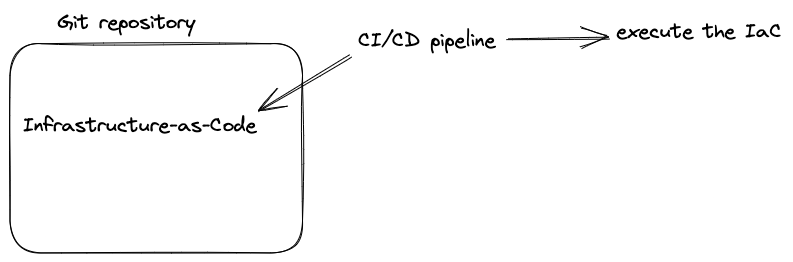
\includegraphics[width=1.00\linewidth]{assets/iac-is-not-gitops.png}
	\caption{IaC is not GitOps.
		%		(\citeauthor{ref}, \citeyear{ref}).
	}
	\label{fig:iacIsNotGitOps}	
\end{figure}

To avoid confusion with what GitOps actually is, 
the OpenGitOps project
\autocite{openGitOpsProject}
was created within the CNCF;
which is maintained by the GitOps working group.

The overall goal of OpenGitOps is to establish a clear vendor-neutral,
principle-driven meaning of GitOps,
which shall provide a foundation for interoperability between tools, conformance and certification through enduring programs, documents and code
\autocite{opengitopsDocuments}.

The definition of GitOps as per the OpenGitOps project
is stated in section \ref{theoretical-background:general-definitions} of this thesis.

In fig. \ref{fig:gitOpsConcept} a visual representation can be seen of the main GitOps concept.

\begin{figure}[h]
	\centering
	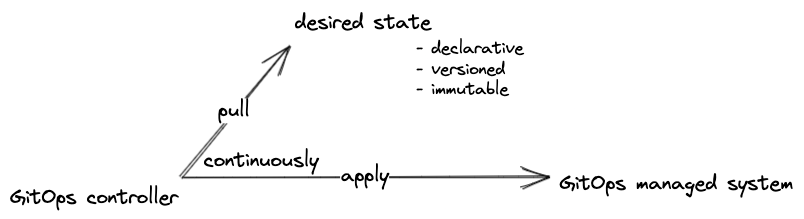
\includegraphics[width=1.00\linewidth]{assets/gitops-concept.png}
	\caption{GitOps concept.
		%		(\citeauthor{ref}, \citeyear{ref}).
	}
	\label{fig:gitOpsConcept}	
\end{figure}







\section{How GitOps changed Continuous Delivery}
\label{theoretical-background:gitops-cd}

Before GitOps, Continuous Delivery was primarliy push-based.
This means that a code change is introduced by a developer,
this code change is commited to a Git repository.
Then a CI/CD system gets triggered to execute a certain pipeline
of jobs.
These jobs may be to test the code and build an artifact, push the artifact
to a registry, etc.
The jobs are run in a pipeline - one after the other -
if one fails, the pipeline is cancelled.
The commit, that is a new version of the code -
is pushed through the pipeline.
Eventually at the end of the pipeline
the new version is deployed by pushing the new artifact
to the deployment environment in an imperative way.
Once the new version is deployed, the pipeline stops.

\begin{figure}[h]
	\centering
	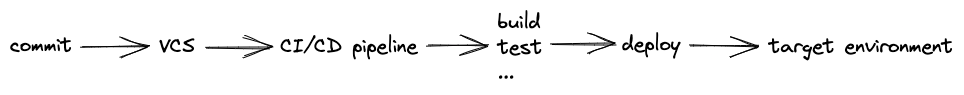
\includegraphics[width=1.00\linewidth]{assets/push-based-cd.png}
	\caption{Push based Continuous Delivery.
		%		(\citeauthor{ref}, \citeyear{ref}).
	}
	\label{fig:pushBasedCD}	
\end{figure}

With GitOps, this primarily push-based process has changed.
Namely, the last couple of steps when the new version
is deployed to the target environment,
are done asynchronously.
With a GitOps workflow,
the CI/CD pipeline usually stops when the new artifact
is successfully pushed to the artifact registry,
or the desired state is changed in the Git repository.
Then another system - the GitOps controller,
which usually lives inside the deployment environment -
notices that the desired state changed and has now
drifted from the actual state.
The GitOps controller then reconciles the new desired state,
by applying it to the managed system.

\begin{figure}[h]
	\centering
	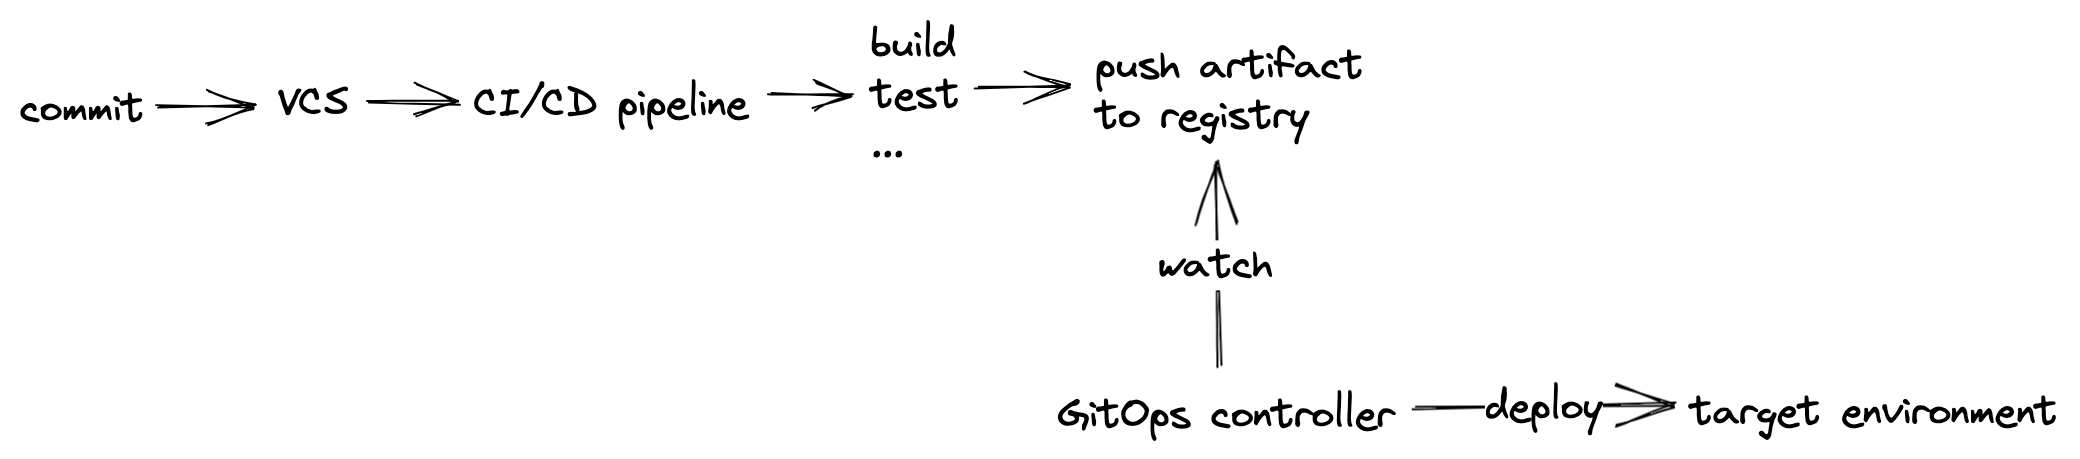
\includegraphics[width=1.00\linewidth]{assets/cd-gitops.png}
	\caption{Continuous Delivery with GitOps.
		%		(\citeauthor{ref}, \citeyear{ref}).
	}
	\label{fig:cd-gitops}	
\end{figure}

One major difference is that with the GitOps workflow,
the CI/CD system no longer knows if and where the application is being
deployed to, since the pipeline usually stops after successful push to the artifact registry.
The desired state, which is stored in a Git repository is continuously being watched
by the GitOps controller. Any changes that it detects are promptly applied to the
target environment.











\section{Promoting Releases Across Environments}

With the push-based pipelines, described in section
\ref{theoretical-background:gitops-cd},
it is typically more straight-forward of how an application
is deployed to multiple target environments.
When the pipeline job to deploy to environment A was successfully done,
the next job to deploy to environment B would be executed.
Since the push-based workflow was a synchronous process from commit
to deployment to target environment,
the whole process could be packed into a single pipeline.

However, with the GitOps workflow the process from
commit to deployment to target environment is usually split up after
publishing of the artifact to the artifact registry.
At this point, the process continues asynchronously.

There are multiple ways how the promotion across environments can be achieved.
In the simplest form, the desired state could be stored in a Git repository,
and the GitOps engine would synchronize every new commit, which is detected -
meaning each and every new change to the desired state is immediately
applied to the actual system state.
For each environment, there would be a representing folder in the Git repository,
or a separate repository.
On every new commit, the reconciliation immediately happens.
It could also be done differently, in that the state or source controller
is configured to watch a specific git refspec, meaning a certain Git tag, for example.
This way, not every commit is deployed, but rather only specific Git tags,
which may be created manually by a human.
When having the desired state as fixed Git tags,
it can possibly provide for more control over what is deployed.

Additionally to leveraging Git tags as fixed and immutable versions,
the desired state could be packaged and pushed to an artifact registry.
Especially when using configuration or templating tools like Kustomize or Helm,
where the Kubernetes manifests need to be rendered before being applied,
it could make sense to go with this approach.
Packaging the desired state into an immutable artifact can also increase
security, when the artifact is signed with a digital signature, and also validated upon deployment.

Whether the desired state is packaged as an artifact with an immutable version and signed signature,
or just stored in a Git repository and secured purely by the built-in Git commit functionality, providing
unique snapshots, which can be rolled back any time;
it always comes down to changing plain text files stored somewhere.
For promotion to other environments, these changes are typically done again for the desired state of the other environment.
There is no way around changing files in Git repositories, as this is within the nature of the GitOps approach.






\section{Towards Progressive Delivery \& Short-Living Environments}

With progressive delivery tools like
Flagger
\autocite{flaggerWebsite}
and
Argo Rollouts
\autocite{argoRolloutsWebsite},
which offer advanced deployment strategies
like canary and blue/green deployments, or A/B testing,
it is now easier to ensure a bad release does not impact the end users
as drastically.
As an example, the named tools make it possible to release new versions
to 10 percent of a specific region of end users,
then this canary rollout is automatically tested and evaluated against metrics,
if certain objectives for metrics fail to be met,
the new release can automatically be rolled back.

\begin{figure}[h]
	\centering
	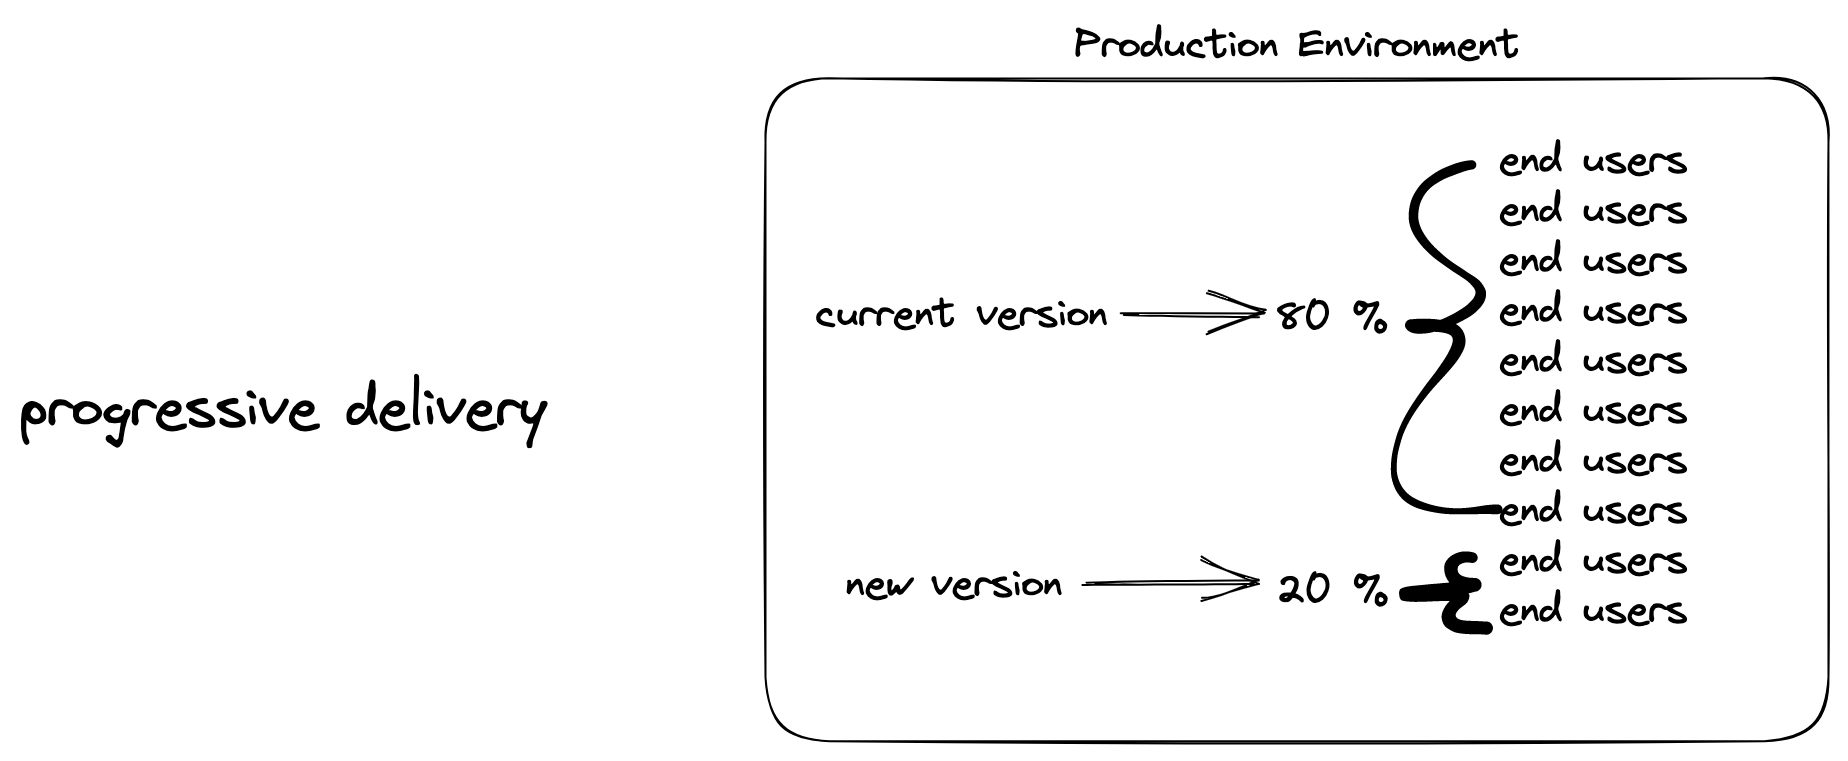
\includegraphics[width=1.00\linewidth]{assets/progressive-delivery.png}
	\caption{Progressive Delivery.
		%		(\citeauthor{ref}, \citeyear{ref}).
	}
	\label{fig:progressive-delivery}	
\end{figure}

Since the progressive delivery tools allow for a more
fine-grained segmentation
of a single environment based on numerous parameters like
client device type, user region, user type (e.g., developer, admin),
registered or unregistered users, etc.
the requirements to have a multitude of deployment environments
have decreased for some organizations.
An illustration can be seen in fig. \ref{fig:progressive-delivery}.

The described segmentation of an environment with the progressive delivery
tools, however might not be possible for every use case or organization.
Financial institutions for example, where the requirement for absolutely zero
errors hitting the production environment is top priority and business critical,
to say the least,
may still want to run multiple environments next to progressive delivery tools,
to ensure an even higher quality and level of caution.
This is illustrated in fig. \ref{fig:deploy-multiple-envs}.

Multiple environments typically mean a big increase in costs;
with progressive delivery the need for multiple environments has decreased,
and this way costs can be reduced.

\begin{figure}[h]
	\centering
	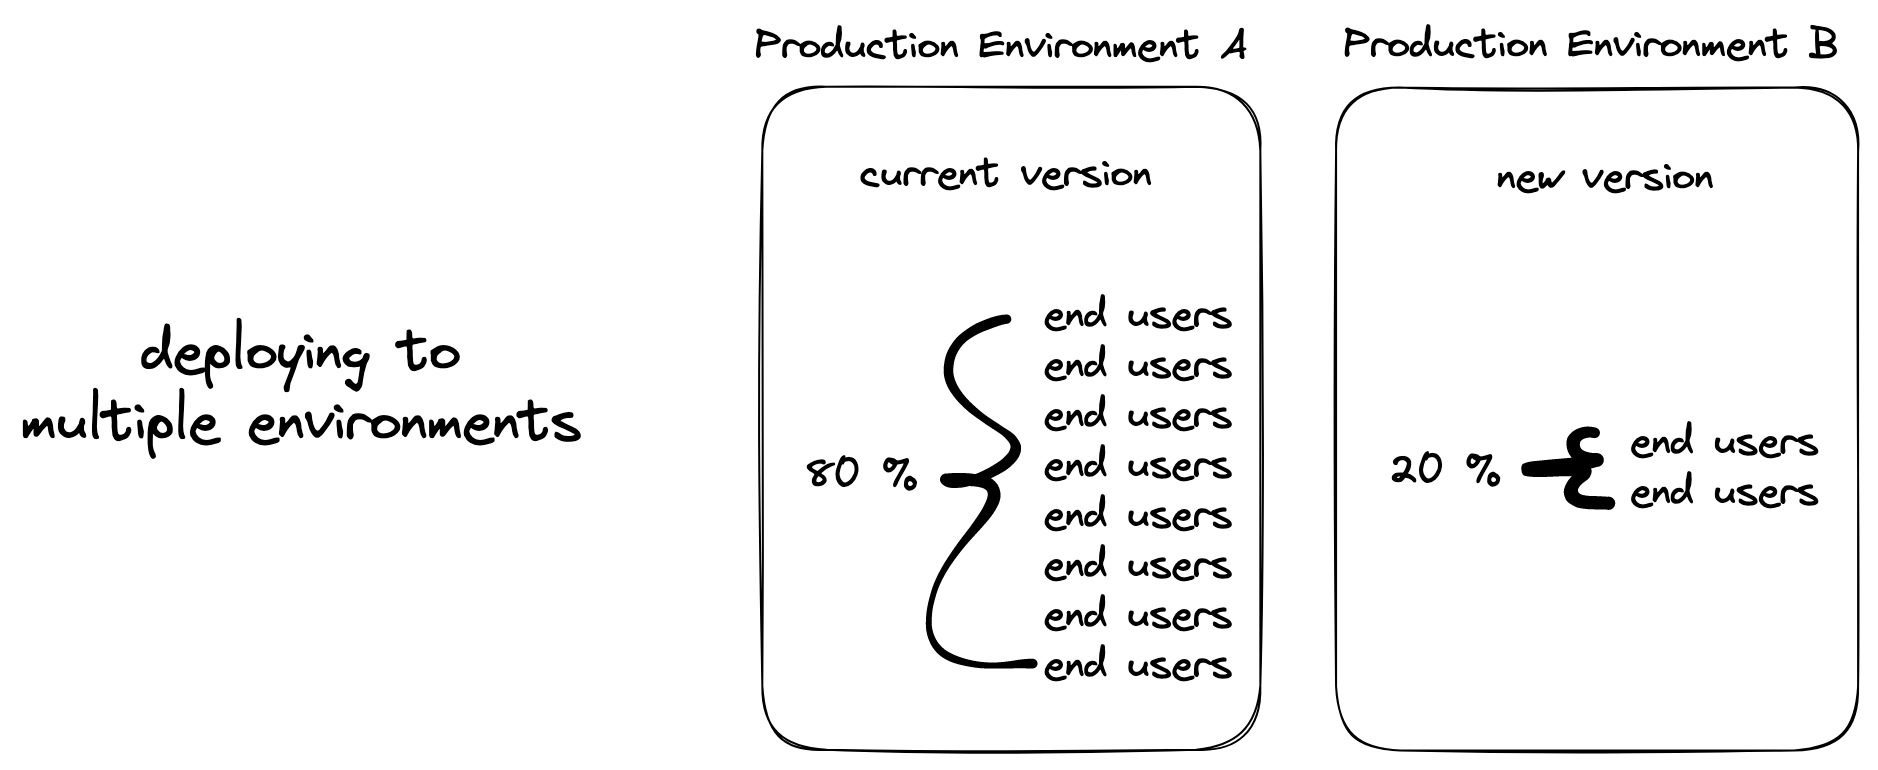
\includegraphics[width=1.00\linewidth]{assets/deploy-multiple-envs.png}
	\caption{Deploying to multiple environments.
		%		(\citeauthor{ref}, \citeyear{ref}).
	}
	\label{fig:deploy-multiple-envs}	
\end{figure}

Nowadays with the rapid development and releasing of new versions,
there has become a need for dynamic, short-living environments.
For every commit of an individual developer,
a deployment environment may be provisioned for previewing the changes
in a live environment that resembles the production environment as well as possible.
This short-living environment may be deleted after a short specified amount of time
has passed.






\section{Beyond container orchestration with Kubernetes}
\label{theoretical-background:kubernetes}

The following section is about
the role Kubernetes plays in the current cloud native ecosystem,
and its extensible architecture.

Since the birth of the cloud native computing foundation (CNCF) in 2015 and the release of Kubernetes as the first CNCF project,
there have emerged more than a hundred projects.
Most of the projects are hosting cloud native technologies and tools to support Kubernetes.
The current ecosystem and toolchains are strongly centered around Kubernetes,
although not strictly tied to it and often times with the explicit effort
for the ability to support alternative cloud native platforms and solutions.

\enquote*{Kubernetes, also known as K8s, is an open-source system for automating deployment, scaling, and management of containerized applications.}
\autocite{kubernetesIoWebsite}
Although this is the primary use case of Kubernetes,
and the reason why it was created initially,
Kubernetes is increasingly being used as a base cloud native platform,
to build other applications and platforms on top of.
The architecture of Kubernetes provides a solid framework and platform,
which is easily extensible.
Developers may extend its API by specifying custom resources and controllers.

There are several advantages when extending the Kubernetes API,
in comparison to a plain REST API.
Some of those are the following
\autocite{kubebuilderBookWebsite}:

\begin{itemize}
	\item \enquote*{Hosted API endpoints, storage, and validation.}
	\item \enquote*{Rich tooling and clis such as kubectl and kustomize.}
	\item \enquote*{Support for Authn and granular Authz.}
	\item \enquote*{Support for API evolution through API versioning and conversion.}
	\item \enquote*{Facilitation of adaptive / self-healing APIs that continuously respond to changes in the system state without user intervention.}
	\item \enquote*{Kubernetes as a hosting environment}
	\autocite{kubebuilderBookWebsite}
\end{itemize}

When developing a Kubernetes-native application,
many of the common capabilities which are often required for all applications,
are being provided by Kubernetes itself, or otherwise easily consumable and integrated.
These may include resource quotas, observability, monitoring, logging and tracing,
configuration state storage, declarative APIs, control loops, and event and message queueing.

\subsection*{Extending Kubernetes}
% https://kubernetes.io/docs/concepts/extend-kubernetes/
Kubernetes offers several different extension points and extension patterns.
Most extension patterns however share the same basic design and principles.
In general, a custom extension is a program which reads and/or writes
to the Kubernetes API. By doing that it can provide useful automation.
Since Kubernetes is based around a declarative API,
where resources are defined as the desired state,
and controllers are responsible for continuously reconciling this
desired state with the actual state,
it has shown to be a good pattern to design custom extensions in the same way
\autocite{extendKubernetes}.

\subsection*{Custom Resources, Controllers and Operators}
% https://kubernetes.io/docs/concepts/architecture/controller/
The concept of a controller and control loop within Kubernetes refers to the
meaning from robotics and automation, where
\enquote*{a control loop is a non-terminating loop that regulates the state of a system.}
\autocite{controllersKubernetes}
Controllers in Kubernetes are continuously running in a control loop,
in specified intervals and sometimes internal or external triggers, 
and watch the actual state of the cluster,
and make changes to it by interacting with the API,
in order to bring the actual state closer to the desired state,
like specified in the declarative definition.
It is typically a good practice to have one controller
be responsible for one resource, 
in order to help with separation of concerns.
Controllers make changes to resources inside the cluster,
like pods and deployments,
but can also be responsible for resources external to the cluster,
like APIs of the infrastructure provider
\autocite{controllersKubernetes}.
A typical controller implementation can be seen in figure
\ref{fig:typicalControllerKubernetes}.
As an example here, the deployment controller continuously ensures the desired state
of three replicas; if it notices the desired state and actual state differ
from one another, it does necessary actions to make them match again.

\begin{figure}[h]
	\centering
	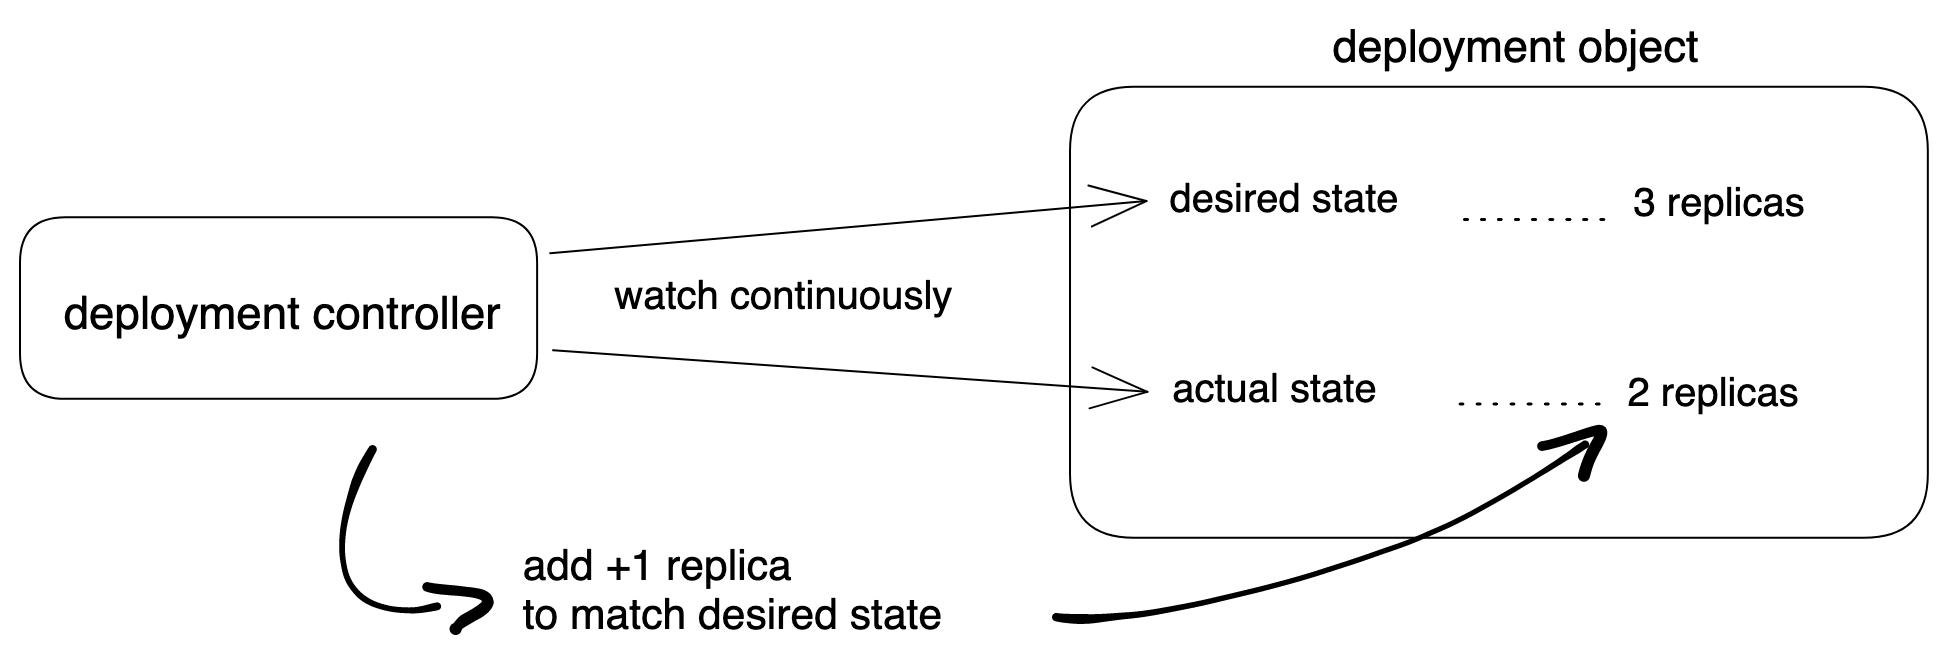
\includegraphics[width=1.00\linewidth]{assets/typical-controller.png}
	\caption{typical controller in Kubernetes.
		%		(\citeauthor{ref}, \citeyear{ref}).
	}
	\label{fig:typicalControllerKubernetes}	
\end{figure}

When a controller has specific domain knowledge,
or does certain tasks, which would usually be done by a human "operator",
it is called an operator.

% https://kubernetes.io/docs/concepts/extend-kubernetes/operator/
Operators typically are a set of controllers and custom resources
with specific codified domain knowledge.
All operational tasks -
which would otherwise have to be done by a human operator -
are written in code.
This code, the controller logic, can then be automated.
Examples for such operational tasks are
backups and restoring of backups, error remediation, database migrations, etc.
\autocite{operatorWhitepaperV1}.
In overly simplified terms:
An operator is a controller plus domain-specific operational knowledge
(fig. \ref{fig:operatorAndController}).

\begin{figure}[h]
	\centering
	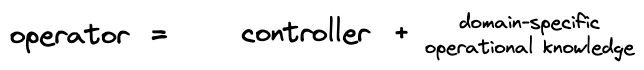
\includegraphics[width=0.85\linewidth]{assets/operator-is-controller-domain-knowledge.png}
	\caption{Operator and Controller.
		%		(\citeauthor{ref}, \citeyear{ref}).
	}
	\label{fig:operatorAndController}	
\end{figure}

The Operator Design Pattern represents a set of principles about
managing complex applications and/or infrastructure resources,
using domain-specific knowledge.
The goal is to limit any manual work that needs to be done,
and try to automate all operational tasks.
This is done by capturing domain-specific knowledge in code,
defining the desired state of resources and exposing them
via a declarative API
\autocite{operatorWhitepaperV1}.

To simplify the process of creating and maintaining Kubernetes-native application
in the form of an operator,
there exist several operator frameworks.
The most prominent framework is the Kubebuilder Framework.
%\url{https://github.com/kubernetes-sigs/kubebuilder}
The Kubebuilder framework makes the process of extending the Kubernetes API
an easy process for developers.
An initial project can easily be boostrapped, allowing the developer to focus
on implementing the custom resource definitions and controller logic.
Any needed Kubernetes primitives, such as service accounts and RBAC permissions
are automatically generated.
Documentation for the OpenAPI resources are also generated from the code,
which is the Go programming language.
There exist rich libraries for interfacing with Kubernetes components,
since Kubernetes itself is also implemented in the Go language
\autocite{kubebuilderBookWebsite}.

With custom resources, the Kubernetes API can dynamically be extended during runtime,
without the need to access its source code or recompile it.

While a resource is
\enquote*{an endpoint in the Kubernetes API that stores a collection of API objects of a certain kind}
\autocite{customResourcesKubernetesIO},
a custom resource is
\enquote*{an extension of the Kubernetes API that is not necessarily available in a default Kubernetes installation}
\autocite{customResourcesKubernetesIO}.
Custom resources can be dynamically registered and independently updated.
Users can interface with its objects as they do with the Kubernetes built-in resources
\autocite{customResourcesKubernetesIO}.









\section{Modeling GitOps Environments}

GitOps environments as defined in section
\ref{theoretical-background:general-definitions},
are currently being modeled using different approaches.
The most prominent approach is to have a folder in a Git repository
per environment. This is straight-forward and easily compatible with
the currently most used configuration and templating tools like Kustomize and Helm.
Promotion would be just a file copy operation from one to another file or folder.
For each environment, or only critical ones, there could be a completely separate Git repository.
Having a separate repository opens up the possibility to have a more strict separation of concerns,
regarding permissions and access rights.
Anyone who has access to a Git repository has read access to the entire repository tree.
While the write access could potentially be limited by administrators or maintainers
to certain folders, the read access will always be open for anyone who has access to the repository.

Another approach is to have a Git branch per environment.
Promotion would be a Git merge from one to another branch.
When taking this approach, and also having environment-specific configuration,
it is possible, when not being careful, that a merge conflict happens,
and the promotion would need to be solved manually.
However when this approach is purely used for the purpose of staging,
meaning environments are identical, but new releases are deployed to some environments first
after other ones,
it could provide a seamless way of promotion by solely leveraging the built-in merge mechanism in Git.
Branches can usually be restricted or limited to certain developers only,
which would make it easier to implement the access permissions than the previous folder-per-environment approach.

This research focuses primarily on the modeling of folder-per-environment.








\section{Promotion Strategies with Existing Tools}

There are many ways for achieving a promotion process when using the GitOps approach for the Continuous Delivery of
an application or any other infrastructure declared in code.
When a push-based CI/CD pipeline is already in place, it is often the first thing that comes to mind
to just append the GitOps deployment as a synchronized process to the end of the pipeline.
GitOps engines like ArgoCD offer the capability for the user to configure webhook receivers
which reconcile an application. This makes it possible to setup a synchronous pipeline,
which results in every code change being delivered through a pipeline step by step in a synchronous manner.
After the push-based synchronous deployment step succeeds in the pipeline process,
the pipeline developer can configure another imperative step which triggers reconcilication for another environment.

However, there is a downside when choosing to go with such a push-based imperative approach.
In fact, this approach would abide by the core principles of GitOps,
namely the principle of desired state being continuously being pulled by the GitOps engine/agent.
So the advantage of drift detection and automatic mending, would no longer be given.

When following the GitOps approach, it may be desirable to decouple Continuous Integration/Delivery and Continuous Deployment.
This means that a code change, namely a Git commit, triggers a Continuous Integration pipeline,
which ends in a step which builds and pushes an artifact of the new version to an artifact registry.
The pipeline ends at this point.
Afterwards the GitOps engine, another system than the CI/CD system, is responsible for detecting the new desired state and starting reconciliation.
However, the desired state first needs to be changed after a new artifact is available,
and especially when multiple environments are needed and promotion should be achieved between them,
this is not straight-forward with this asynchronous process.
It may be desirable to trigger tests after a deployment to a certain environment is done,
and only afterwards promote to another environment.
The GitOps approach proposes to have the source of truth in the Git repository as the desired state of a system.

Currently there is insufficient tooling in the GitOps ecosystem for streamlining such a
multi-environment promotion process.

{\color{red}\larger TODO review section!}



















\section{Summary}

TODO































%
%\section{Instruction included in the original FHBgld word processor template}
%\subsection{General definitions}
%Die in dieser Formatvorlage beispielhaft enthaltenen Überschriften sind auf die im
%konkreten Fall tatsächlich passenden Überschriften anzupassen.
%In diesem Teil der Arbeit werden die zum eindeutigen Verständnis unbedingt
%erforderlichen Grundlagen und Definitionen sowie die Erklärung wichtiger Begriffe
%angeführt.
%Die Gliederungspunkte müssen möglichst prägnant bezeichnet werden.
%\subsection{Related work / state of research}
%Auch die neuesten Entwicklungen und Arbeiten auf diesem Gebiet (Stand der
%Wissenschaft oder auch state-of-the-art) sind darzulegen, wobei diese je nach Thema
%auch in der 1. Gliederungsebene behandelt werden können.
%
%\section{Ordinary text}
%% A '%' character causes TeX to ignore all remaining text on the line,
%% and is used for comments like this one.
%
%% sections are begun with similar 
%% \subsection and \subsubsection commands.
%
%The ends  of words and sentences are marked by spaces. It doesn't matter how many 
%spaces    you type; one is as good as 100.  The
%end of   a line counts as a space.
%
%One   or more   blank lines denote the  end 
%of  a paragraph.  
%
%Since any number of consecutive spaces are treated
%like a single one, the formatting of the input
%file makes no difference to
%\LaTeX,                % The \LaTeX command generates the LaTeX logo.
%but it makes a difference to you.  When you use 
%\LaTeX \cite{lamport94},  % \cite inserts a reference, which you define at the end of the document
%making your input file as easy to read
%as possible will be a great help as you write 
%your document and when you change it.  This sample 
%file shows how you can add comments to your own input 
%file.
%
%Because printing is different from typewriting,
%there are a number of things that you have to do
%differently when preparing an input file than if
%you were just typing the document directly.
%Quotation marks like
%``this'' 
%have to be handled specially, as do quotes within
%quotes:
%``\,`this'            % \, separates the double and single quote.
%is what I just 
%wrote, not  `that'\,''.  
%
%Dashes come in three sizes: an 
%intra-word 
%dash, a medium dash for number ranges like 
%1--2, 
%and a punctuation 
%dash---like 
%this.
%
%A sentence-ending space should be larger than the
%space between words within a sentence.  You
%sometimes have to type special commands in
%conjunction with punctuation characters to get
%this right, as in the following sentence.
%Gnats, gnus, etc.\ all  % `\ ' makes an inter-word space.
%begin with G\@.         % \@ marks end-of-sentence punctuation.
%You should check the spaces after periods when
%reading your output to make sure you haven't
%forgotten any special cases.  Generating an
%ellipsis
%\ldots\               % `\ ' is needed after `\ldots' because TeX 
%% ignores spaces after command names like \ldots 
%% made from \ + letters.
%%
%% Note how a `%' character causes TeX to ignore 
%% the end of the input line, so these blank lines 
%% do not start a new paragraph.
%%
%with the right spacing around the periods requires
%a special command.
%
%\LaTeX\ interprets some common characters as
%commands, so you must type special commands to
%generate them.  These characters include the
%following:
%\$ \& \% \# \{ and \}.
%
%In printing, text is usually emphasized with an
%\emph{italic}  
%type style.  
%
%\begin{em}
%	A long segment of text can also be emphasized 
%	in this way.  Text within such a segment can be 
%	given \emph{additional} emphasis.
%\end{em}
%
%It is sometimes necessary to prevent \LaTeX\ from
%breaking a line where it might otherwise do so.
%This may be at a space, as between the ``Mr.''\ and
%``Jones'' in
%``Mr.~Jones'',        % ~ produces an unbreakable interword space.
%or within a word---especially when the word is a
%symbol like
%\mbox{\emph{itemnum}} 
%that makes little sense when hyphenated across
%lines.
%
%Footnotes\footnote{This is an example of a footnote.}
%pose no problem.
%
%\LaTeX\ is good at typesetting mathematical formulas
%like
%\( x-3y + z = 7 \) 
%or
%\( a_{1} > x^{2n} + y^{2n} > x' \)
%or  
%\( AB  = \sum_{i} a_{i} b_{i} \).
%The spaces you type in a formula are 
%ignored.  Remember that a letter like
%$x$                   % $ ... $  and  \( ... \)  are equivalent
%is a formula when it denotes a mathematical
%symbol, and it should be typed as one.
%Furthermore you can add a formula as Images or Tables, see Formula  \hyperref[eq:abc]{\ref{eq:abc}}
%\begin{equation}
%	\label{eq:abc}
%	a+b=c
%\end{equation}
%
%It is sometimes necessary to prevent \LaTeX\ from
%breaking a line where it might otherwise do so.
%This may be at a space, as between the ``Mr.''\ and
%``Jones'' in
%``Mr.~Jones'',        % ~ produces an unbreakable interword space.
%or within a word---especially when the word is a
%symbol like
%\mbox{\emph{itemnum}} 
%that makes little sense when hyphenated across
%lines.

%\chapter{Methodology}

In this chapter,
the methodological approach,
as well as
the used scientific research methods
are presented.


\section{Approach}
\label{methodology:approach}

To achieve the main goal of the thesis and answer the identified research questions,
a mix of different scientific methods will be used.
In order to help with the recognition and legitimization of the conducted research,
a commonly accepted framework, namely
the methodology for conducting design science (DS) research
in information systems (IS)
\autocite{designScienceResearchMethodologyForInformationSystemsResearch}
will be applied.
It consists of six activities
(illustrated in Figure \ref{fig:dsrmProcessReleasePromotionGitOps}):

\begin{itemize}
	\item \nameref{methodology:activity1}
	\item \nameref{methodology:activity2}
	\item \nameref{methodology:activity3}
	\item \nameref{methodology:activity4}
	\item \nameref{methodology:activity5}
	\item \nameref{methodology:activity6}
\end{itemize}

%Since the model allows for process iteration,
%it will be decided by the researcher
%whether, at the end of activity 5,
%to iterate back to activity 3 to try to improve the artifact.
The process is structured in a nominally sequential order.
For this concrete research,
the problem-centered initiation is chosen as the entry point,
thus the process will begin with activity 1.
Afterwards the research will proceed sequentially,
because the idea of the research resulted from observation of the problem
\autocite{designScienceResearchMethodologyForInformationSystemsResearch}.
\bigskip

% TODO: add activity 1-6 to illustration?

\begin{figure}[h]
	\centering
	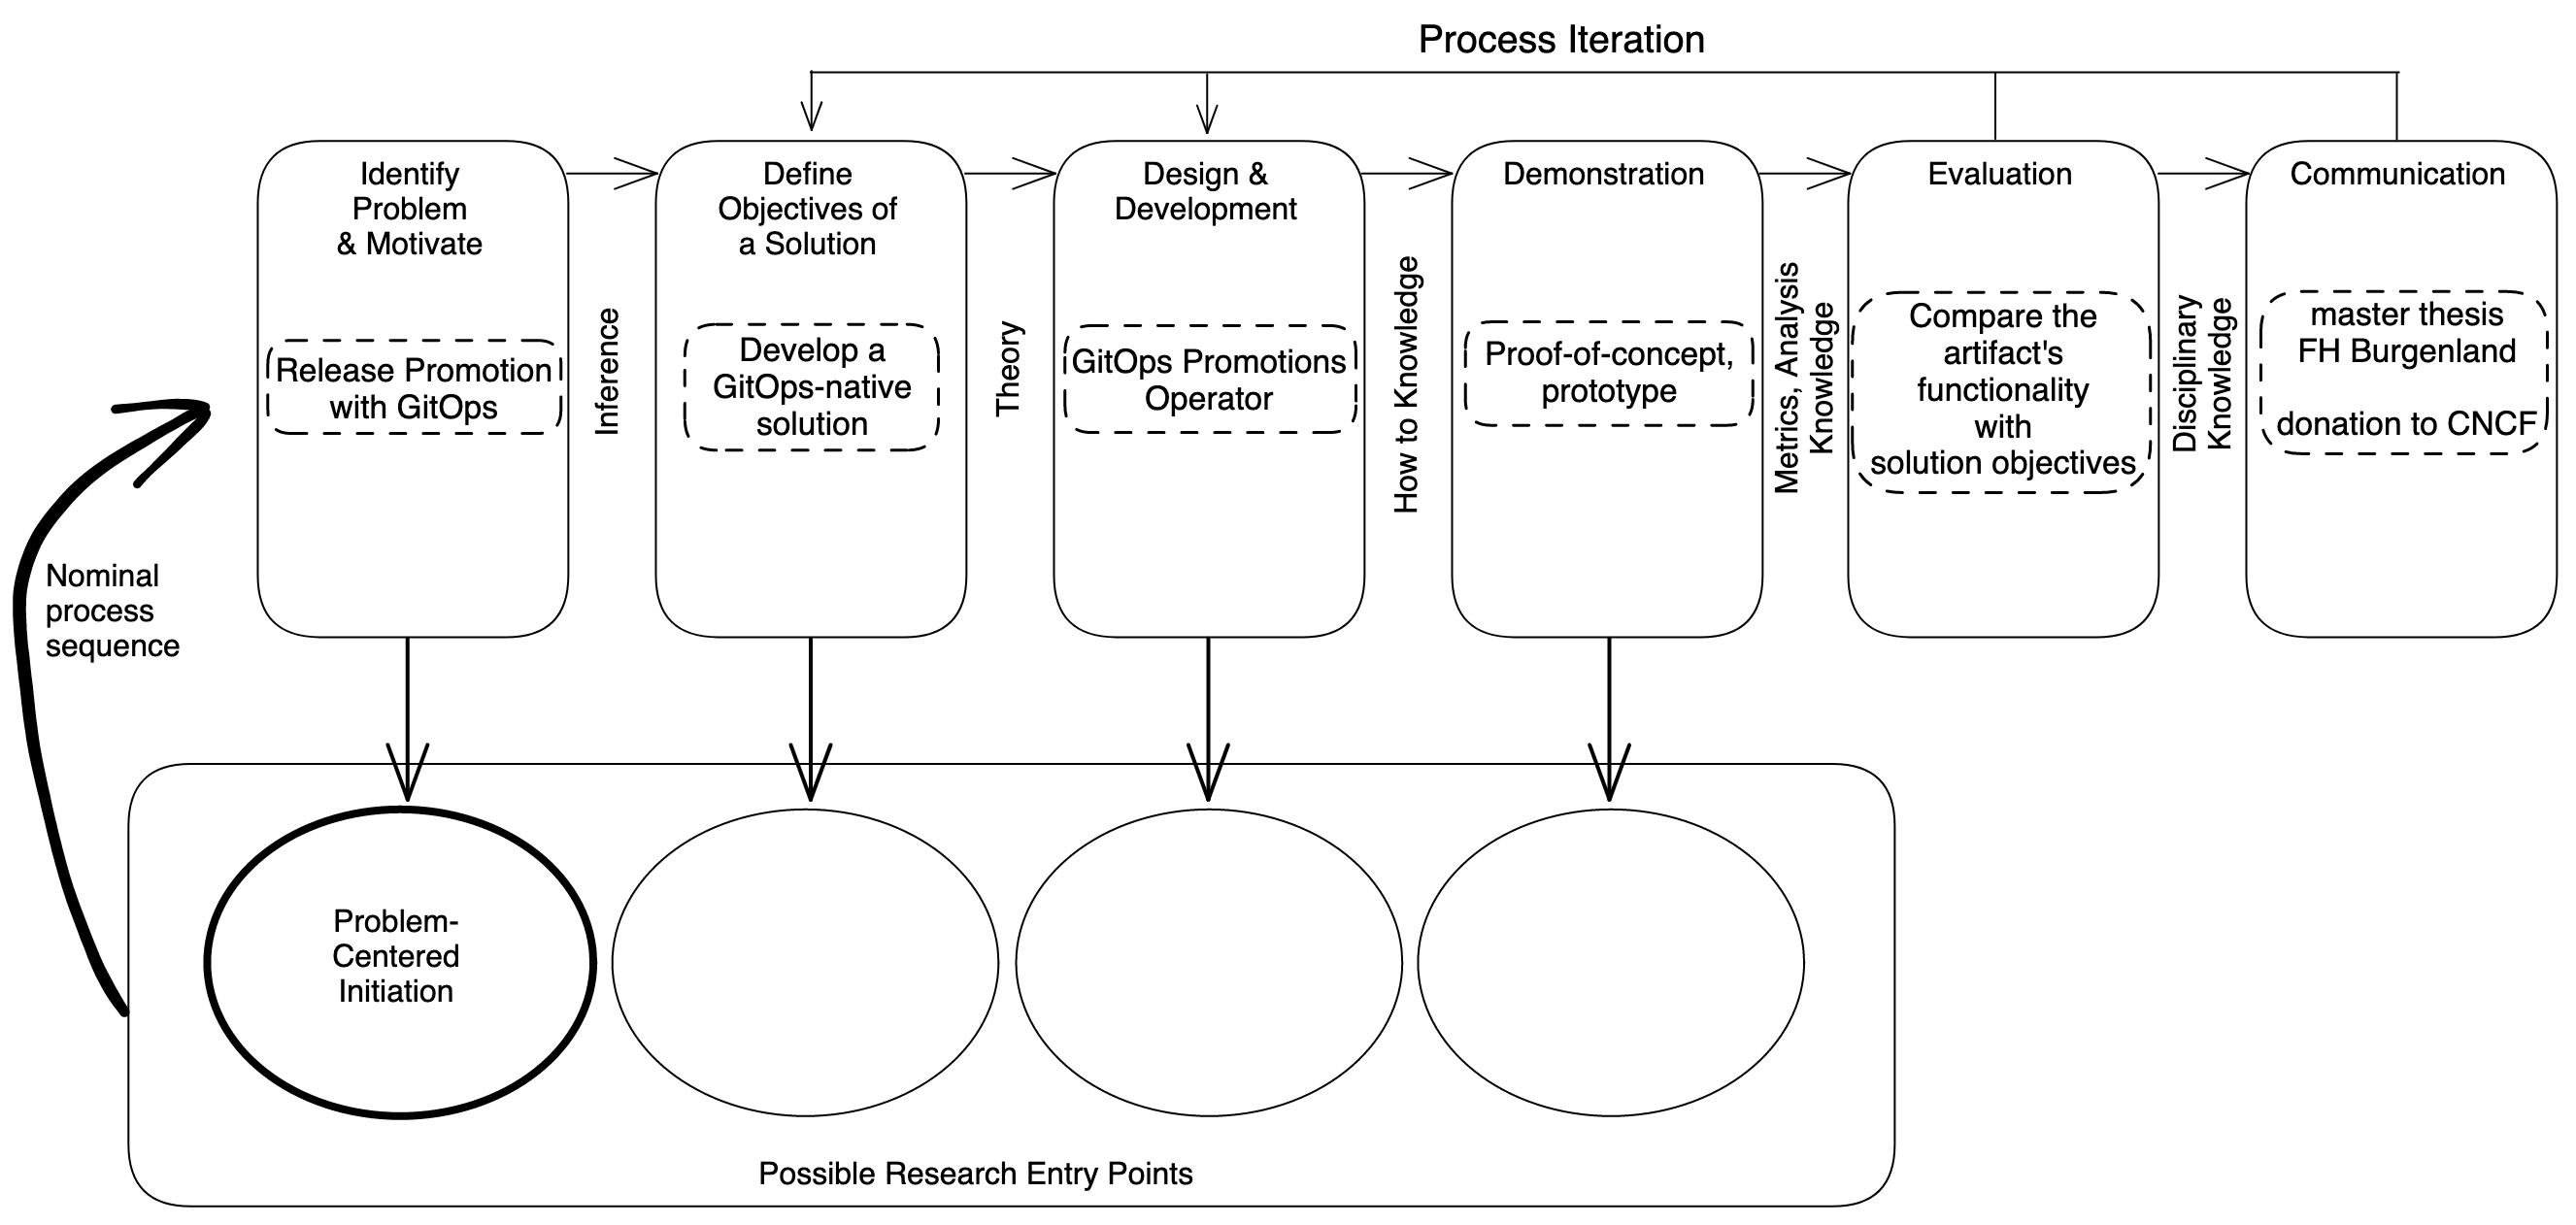
\includegraphics[width=1.00\linewidth]{figures/dsrm-process-release-promotion-gitops.png}
	\caption{DSRM Process for this thesis.
		%		(\citeauthor{ref}, \citeyear{ref}).
	}
	\label{fig:dsrmProcessReleasePromotionGitOps}	
\end{figure}

\subsection{Activity 1: Identify Problem \& Motivate}
\label{methodology:activity1}

\noindent
In activity 1,
the research problem of
release promotion with GitOps
is defined.
This is accomplished, by
seeking knowledge of the state of the problem
from practicing professionals.
This is done by conducting
semi-structured interviews, as described in section \ref{methodology:interview},
as well as analysing prior written literature.
To assist later evaluation,
the problem is conceptually broken down into distinct items.
The value of a solution is highlighted,
in order to help the audience of the research
understand the reasoning associated with the
researcher's understanding of the problem
\autocite{designScienceResearchMethodologyForInformationSystemsResearch}.
\bigskip

\begin{figure}[h]
	\centering
	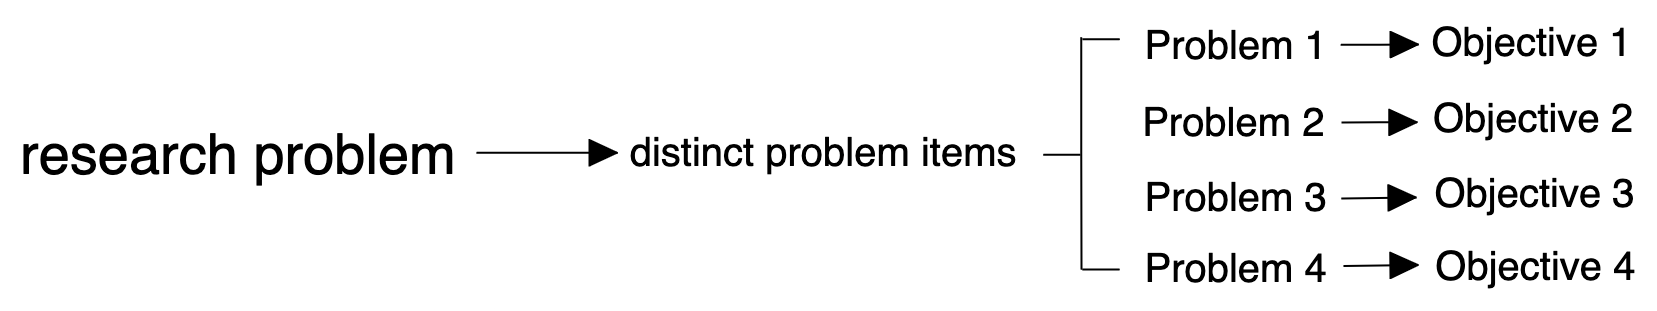
\includegraphics[width=0.75\linewidth]{assets/problem-to-objective-mapping.png}
	\caption{Inference of objectives from problems.
		%		(\citeauthor{ref}, \citeyear{ref}).
	}
	\label{fig:problemToObjectiveMapping}	
\end{figure}

\subsection{Activity 2: Define Objectives of a Solution}
\label{methodology:activity2}

\noindent
In activity 2,
research objectives are inferred from the problem definition in activity 1.
Each objective maps to a distinct item from the problem specification
(illustrated in Figure \ref{fig:problemToObjectiveMapping}),
which helps with later evaluation in activity 5.
In practice, a research objective will be a qualitative description of
how a new artifact is expected to support a solution to the problem definition.
\bigskip

\subsection{Activity 3: Design \& Development}
\label{methodology:activity3}

\noindent
In activity 3,
solutions for the previously defined objectives are designed and developed
by means of producing an artifact.
This is achieved by
determining the artifact's desired functionality and its architecture,
followed by actually creating the artifact
\autocite{designScienceResearchMethodologyForInformationSystemsResearch}.
In practice this means that:
Abstract model definitions are designed;
with the specification of the model definitions in place,
the "release promotion operator" is developed as an artifact.
\bigskip

\subsection{Activity 4: Demonstration}
\label{methodology:activity4}

\noindent
In activity 4,
the in-context use of the artifact is demonstrated.
After outlining how to use the artifact to effectively provide a solution to the problem definition,
the artifact is implemented in a proof-of-concept-level prototype.
%In practice,
%the prototype 
\bigskip

\subsection{Activity 5: Evaluation}
\label{methodology:activity5}

\noindent
In activity 5,
the implementation of the artifact,
and how well it supports a solution to the problem,
is evaluated.
This is achieved by
comparing the objectives of a solution to actual observed results
from use of the artifact in the demonstration
\autocite{designScienceResearchMethodologyForInformationSystemsResearch}.
In practice this means, that
the functionality of the artifact implemented in the prototype in activity 4,
is compared with the solution objectives from activity 2.
\bigskip

\subsection{Activity 6: Communication}
\label{methodology:activity6}

\noindent
In activity 6, as a final step,
the whole conducted research is communicated by means of
disclosing
the problem and its importance,
the artifact and its utility and novelty,
and the demonstration accompanied by the evalution results
\autocite{designScienceResearchMethodologyForInformationSystemsResearch},
within the publication of a master thesis at
the University of Applied Sciences Burgenland \autocite{fhBurgenlandWebsite}.
In addition, it is communicated to relevant audiences such as
the GitOps Working Group \autocite{gitopsWG} of the CNCF.






\section{Research methods}

In the following section,
the used research methods
semi-structured interview
by
\citeauthor{glaser2010experteninterviews} (\citeyear{glaser2010experteninterviews})
and
design science research methodology for information systems
by
\citeauthor{designScienceResearchMethodologyForInformationSystemsResearch} (\citeyear{designScienceResearchMethodologyForInformationSystemsResearch})
are explained in detail.
%The procedure in the course of the research work is also described.




\subsection{Semi-structured Interview}\label{methodology:interview}

For \nameref{methodology:activity1},
semi-structured interviews with working professionals
are conducted.
For this research method,
the suggested practices and guidelines from
the textbook of
\citeauthor{glaser2010experteninterviews} (\citeyear{glaser2010experteninterviews})
are used.
These interviews have the primary goal of aiding with
problem identification and motivation,
because prior written scientific literature is insufficient on the topic.
For conducting the interviews,
a semi-structured interview guide (Appendix \ref{appendix:interview-guide}) is used.

The interview guide is created on the basis of preliminary theoretical considerations.
The use of a guide facilitates the comparability of several interviews,
but still leaves enough room for spontaneous statements.
The advantage of a guide is that the researcher can stick to concrete questions.
Follow-up questioning is allowed and the questions are mostly open.
The open questioning enables the interviewee to present their point of view
\autocite{berger2016wissenschaftliches}.


\subsubsection*{Preparing the Interviews}

As an initial step,
a semi-structured interview guide is developed.
It serves as a rough guideline for the structure of the interview process.
Additionally it encompasses the content-related interview questions,
which are specific to the given research problem.
These questions can be seen at section \ref{appendix:interview-questions} in the appendix.

The selection of the interview partners is based on the questions mentioned in
\citeauthor{glaser2010experteninterviews} (\citeyear{glaser2010experteninterviews}):

\begin{itemize}
	\item Who has the information relevant to this work?
	\item Who can describe it precisely?
	\item Who is most willing to be interviewed?
	\item Who is available?
\end{itemize}

The pool of potential interview partners is mainly oriented around
contacts from friends and acquaintances,
who are working professionally in the GitOps field.
The contact to the interview partners is done via Slack \autocite{slackWebsite} or e-mail.
Prior to conducting the interview, the interview guide is sent to the interviewee.

\subsubsection*{Conducting the interviews}

Appointments for the interviews are made with each interview partner in advance. 
Eventually, the interview is conducted with a web video conferencing tool like Zoom \autocite{zoomWebsite}.
The interviews are recorded for later transcription.
The semi-structured interview guide
is used as a guideline for the interview process as a whole.
However, the actual structure of the interview may differ for each individual interview and according interview partner.

\subsubsection*{Transcription and post-processing of the interviews}

The output of the interviews are in the form of audio-video recordings.
These are transcribed word-for-word into a written form afterwards.
The transcriptions can be seen in Appendix \ref{appendix:interview-transcriptions}.
The content-related answers of the interview partners are taken into consideration
for \nameref{methodology:activity1}, and there further processed.





\subsection{Qualitative Content Analysis}

For \nameref{methodology:activity2},
the transcriptions of the interviews are evaluated with
the qualitative content analysis by
\citeauthor{mayring2019qualitative} (\citeyear{mayring2019qualitative}).

\subsubsection*{Object and research question}

The underlying object for the content analysis are
the conducted semi-structured interviews as described in section \ref{methodology:interview}.

The research questions are presented in the earlier section \ref{introduction:research-question}.

\subsubsection*{Approach}

As the main approach,
the inductive category formation
is chosen.
The first text passage is read,
then a category is formed,
and finally you proceed to the next passage.
For the next passage,
you decide if an existing category matches
or you need to form a new one.
This process continues until all text passages are handled.
At the end, similar categories may be merged together.

\subsubsection*{Coding}

Each text passage is labelled with the according category.

\subsubsection*{Review of categories}

About halfway through the coding process,
\citeauthor{mayring2019qualitative} (\citeyear{mayring2019qualitative})
advises to review the already formed categories.
The following questions may be asked:
Do they represent the content well?
Were they formed in an appropriate relation?
How do possible denotations look?
Could you merge certain categories?

\subsubsection*{Completion of coding process}

After reviewing the categories,
and taking appropriate measures,
the coding process is completed.

\subsubsection*{Reliability check}

Once coding is completed,
a reliability check is done.
How much do the results differ in replication?
This is achieved by letting another independent researcher
execute the coding process.

%Cohens's Kappa (1960)
%Krippendorff's Alpha (1970)

\subsubsection*{Evaluation and interpretation}

A possible way for evaluation would be to check frequencies.

How often does each of the categories occur in the data set?
What does this mean in terms of my research question?
How do my results relate to the existing state of research?













\subsection{Design Science Research Methodology}

The
design science research methodology (DSRM)
has already been described and applied in the earlier section
\ref{methodology:approach} \nameref{methodology:approach}
of this thesis.

\citeauthor{designScienceResearchMethodologyForInformationSystemsResearch} (\citeyear{designScienceResearchMethodologyForInformationSystemsResearch})
describe DSRM as follows:

\begin{quotation}
\noindent
We propose and develop a design science research methodology (DSRM) for the
production and presentation of DS research in IS. This effort contributes to IS research
by providing a commonly accepted framework for successfully carrying out DS research
and a mental model for its presentation. It may also help with the recognition
and legitimization of DS research and its objectives, processes, and outputs, and it
should help researchers to present research with reference to a commonly understood
framework, rather than justifying the research paradigm on an ad hoc basis with each
new paper.

\noindent
\autocite{designScienceResearchMethodologyForInformationSystemsResearch}
\end{quotation}

\enquote*{DS is of importance in a discipline oriented to the creation of successful artifacts.}
\autocite{designScienceResearchMethodologyForInformationSystemsResearch}


%DSRM provides a nominal process model consisting of six steps:
%problem identification and motivation, definition of the objectives for a solution, design and development, demonstration, evaluation, and communication


















%\section{Approach}
%Alle im durchgeführten Untersuchungen und Versuche müssen systematisch und
%nachvollziehbar sein. Daher ist die gewählte Vorgangsweise genau zu beschreiben
%und zu begründen. Es empfiehlt sich, dafür Literatur zum wissenschaftlichen Arbeiten
%heranzuziehen.
%
%\section{Research methods}
%Die eingesetzte Methoden (z.B. Online-Befragung, Inhaltsanalyse, Interviews) müssen
%ebenfalls nachvollziehbar beschrieben werden.
%Unterschiedliche Untersuchungsmethoden haben oft unterschiedliche Genauigkeit.
%Neben der Begründung und Beschreibung der Untersuchungsmethoden ist auch eine
%Begründung und Beschreibung der verwendeten Auswertungsmethoden bzw. dafür
%verwendete Software unerlässlich\footnote{Wenn der Abstand zwischen Fußnotentrennstrich und Fußnote zu groß wird, gehen Sie folgend vor:
%	Wählen Sie im Hauptmenü „Ansicht | Entwurf | Verweise | Notizen anzeigen |
%	Fußnotentrennlinie". Dann können Sie unnötige Leerzeichen entfernen.
%}.
%Wenn es ein Kapitel 3.2.1 gibt, muss es auch ein Kapitel 3.2.2 geben.

%\subsubsection{<<Überschrift 4. Ebene>>}
%4 Überschriftenebenen müssen reichen.
%
%
%\section{Displayed Text}
%Text is displayed by indenting it from the left
%margin.  Quotations are commonly displayed.  There
%are short quotations
%\begin{quote}
%	This is a short quotation.  It consists of a 
%	single paragraph of text.  See how it is formatted.
%\end{quote}
%and longer ones.
%\begin{quotation}
%	This is a longer quotation.  It consists of two
%	paragraphs of text, neither of which are
%	particularly interesting.
%	
%	This is the second paragraph of the quotation.  It
%	is just as dull as the first paragraph.
%\end{quotation}
%Another frequently-displayed structure is a list.
%The following is an example of an \emph{itemized}
%list.
%\begin{itemize}
%	\item This is the first item of an itemized list.
%	Each item in the list is marked with a ``tick''.
%	You don't have to worry about what kind of tick
%	mark is used.
%	
%	\item This is the second item of the list.  It
%	contains another list nested inside it.  The inner
%	list is an \emph{enumerated} list.
%	\begin{enumerate}
%		\item This is the first item of an enumerated 
%		list that is nested within the itemized list.
%		
%		\item This is the second item of the inner list.  
%		\LaTeX\ allows you to nest lists deeper than 
%		you really should.
%	\end{enumerate}
%	This is the rest of the second item of the outer
%	list.  It is no more interesting than any other
%	part of the item.
%	\item This is the third item of the list.
%\end{itemize}
%You can even display poetry.
%\begin{verse}
%	There is an environment 
%	for verse \\             % The \\ command separates lines
%	Whose features some poets % within a stanza.
%	will curse.   
%	
%	% One or more blank lines separate stanzas.
%	
%	For instead of making\\
%	Them do \emph{all} line breaking, \\
%	It allows them to put too many words on a line when they'd rather be 
%	forced to be terse.
%\end{verse}
%
%Mathematical formulas may also be displayed.  A
%displayed formula 
%is 
%one-line long; multiline
%formulas require special formatting instructions.
%\[  \Gamma \times  \psi = x'' + y^{2} + z_{i}^{n}\]
%Don't start a paragraph with a displayed equation,
%nor make one a paragraph by itself.

%%\chapter{Empirical Work}


\chapter{Interviews with Working Professionals}

\section{Problem Identification \& Motivation}
\section{Definition of Solution Objectives}
\section{Summary}



\chapter{GitOps Promotions Operator Prototype}

This chapter describes the developed prototype,
called the GitOps Promotions Operator.

\section{Design \& Development}

The Design of the GitOps Promotions Operator
is based on the underlying constraints of the Kubebuilder framework,
discussed in section \ref{theoretical-background:kubernetes} of this thesis.
The main constraints the framework comes with, are the
custom resource definition + controller pattern.

\begin{figure}[h]
	\centering
	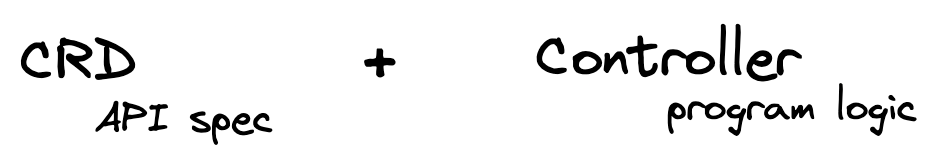
\includegraphics[width=1.00\linewidth]{assets/crd-and-controller.png}
	\caption{Custom Resource Definition and Controller.
		%		(\citeauthor{ref}, \citeyear{ref}).
	}
	\label{fig:crd-and-controller}	
\end{figure}

As the initial step of the design phase,
abstract model definitions are designed.
Their key properties are identified.
Then a sample mockup is designed as
a custom resource definition in Yaml format.
Afterwards this idea of the model definition is 
translated into custom struct types of the
Go programming language,
which is chosen by the Kubebuilder framework.

\subsection{Abstract Models}
	
The first step of the initial design phase is the creation of abstract models.
In order to be able to represent environments and promotions,
the requirement is to at least start with two abstract models for each 
the environment and promotion.

The Environment represents a GitOps environment,
which is a Git repository + path.
The Git repository can be a clone URL to the repository,
and the path is the relative filesystem path, which points to the 
environment, inside the repository.

\begin{figure}[h]
	\centering
	
\includegraphics[width=1.00\linewidth]{assets/gitops-env-repo-and-path.png}
	\caption{GitOps Environment.
		%		(\citeauthor{ref}, \citeyear{ref}).
	}
	\label{fig:gitops-env-repo-and-path}	
\end{figure}

The abstract model for a GitOps environment needs at least the following properties:

\begin{itemize}
	\item URL of the source Git repository
	\item path pointing to the environment inside the repository
\end{itemize}

The URL has the format of a HTTP(S) or SSH URL,
which links to the Git repository,
e.g.:

\begin{itemize}
	\item \lstinline|http://localhost:8080/org/repo|
	\item \lstinline|https://gitprovider.com/org/repo|
	\item \lstinline|ssh://git@gitprovider.com:org/repo|
\end{itemize}

The path has the format of a typical unix style filesystem path.
It starts relative from the root of the given Git repository,
and points to the directory, which represents the GitOps environment.
Examples for a path are the following:

\begin{itemize}
	\item \lstinline|path/to/env|
	\item \lstinline|/path/to/env|
	\item \lstinline|./path/to/env|
	\item \lstinline|./path/to/env/|
\end{itemize}

Note, that these example paths all represent the same directory,
these are just alternative notations.

The abstract model for a GitOps promotion needs at least the following properties:

\begin{itemize}
	\item source environment
	\item target environment
	\item promotion subjects
	\item promotion strategy
\end{itemize}

The source environment defines the environment resource,
where a promotion subject is promoted from.
The target environment defines the environment resource,
where a promotion should promote to.

A promotion subject can be potentially many different things.
In the case of this prototype,
a promotion subject is a file or directory,
which is copied from the source to the target environment.
Examples of such files or directories are the following:

\begin{itemize}
	\item \lstinline|kustomization.yaml|
	\item \lstinline|./component/cert-manager/kustomization.yaml|
	\item \lstinline|./helm-values-prod.yaml|
\end{itemize}

Note, that the relative paths of the promotion subjects,
are relative to the paths of the environment, defined earlier.
An example of the \lstinline|kustomization.yaml|, would look like this:

\lstinline|./path/to/env/kustomization.yaml|

As an example - but outside the scope of the current prototype -
a promotion subject could also be fetched from another source,
like an artifact registry, or be any other type of data
and updated/promoted in the target environment,
e.g. a version tag, helm values, etc.

With the current prototype,
the promotion strategy is to raise a pull request at the Git provider,
with the changes proposed by the promotion.
A human can then review the changes and optionally approve and merge the pull request.
After merging, the promotion will have taken place.

Alternatively to a pull request, the changes could be directly
commited and pushed to the target environment,
without human interaction. This strategy should require different means
of automated or otherwise external or additional checks, in order to ensure a safe promotion.

Now that the abstract models are designed,
they need to be implemented.
Since the decision for the prototype is to be developed
with the Kubebuilder framework and follow its style,
mockups of the custom resources in Yaml format
will be created as a next step.





\subsection{Mockups of Custom Resources}

%to write mockups
%of custom resources in YAML format,
%since this is what the end user will interface with when the application is finished.
%First and foremost the handling and user experience has to be seamless and make sense
%for the user; also it shouldn't take any extra miles for the user to take,
%just to get started.
%The YAML representation of the custom resource should be similar to other ones
%from the Kubernetes core types.

When the abstract models have been specified,
they can be actually implemented with the framework
as Kubernetes custom resource definitions.

Users will mainly be dealing with the custom resources in a Yaml format.
Yaml keys should be intuitive and make sense to the user.
It also helps if they follow the core Kubernetes definitions regarding naming conventions.
An example for a naming convention is the "Ref" suffix for yaml keys.
This suffix is typically appended to keys which represent a reference to another Kubernetes
object.
For example, "secretRef" says that this field refers to a Kubernetes secret resource.

A possible mockup for a GitOps environment -
that is a first prototype implementation of the abstract model into a custom resource -
could look like the following.

\lstinputlisting{assets/files/environment-mockup.yaml}

In this mockup the git reference branch main is also specified \\
in the \lstinline|.spec.source.ref.branch| field.

A possible mockup for a GitOps promotion 
could look like the following.

\lstinputlisting{assets/files/promotion-mockup.yaml}

In the promotion mockup definition,\\
there are four main fields within the \lstinline|.spec|.
These represent the minimum properties of the previously defined abstract definition.
It is to note, that
the \lstinline|.spec.copy| field represents the promotion subjects.
It is a list of items, where each item contains
a \lstinline|name|, \lstinline|source| and \lstinline|target|.
The \lstinline|name| defines a custom name.
The \lstinline|source| and \lstinline|target| fields together define a
file copy operation,
where the \lstinline|source| is the relative path from the source environment,
and the \lstinline|target| is a relative path from the target environment.

\subsection{Alternative Mockups}

The following alternative mockups,
for the custom resource definitions,
i.e. the design of the declarative API,
are suggested, but now implemented in the current prototype.

\subsubsection*{Promotion Subjects defined in each Environment resource}

Alternatively, the promotion subjects could also be specified
in the environment resource.
Then the environment could like the following:

\lstinputlisting{assets/files/environment-mockup-alt-1.yaml}

In the promotion definition,
it would then suffice to specify
a list of promotion subjects.

\lstinputlisting{assets/files/promotion-mockup-alt-1.yaml}

This alternative design allows that each environment could have
a unique path of a specific promotion subject defined.
Now if a promotion is spanning over multiple environments,
they could each specify their own unique path to a promotion subject.
The promotion subject is declared in the promotion,
but the actual path is defined per each environment.

\subsection{Translation to Go types}

Once the mockups of the custom resources in Yaml format are done,
the declarative structure can be translated to custom Go types.

The specification of the Environment resource results in the following code:

\lstinputlisting{assets/files/environmentSpec-type.go}

The type EnvironmentSpec represents the \lstinline|.spec| Yaml field.

What also needs to be defined is the status subresource.
In the status fields, the controller can save the current/actual state
of the resource during runtime.
While \lstinline|.spec| defines the desired state,
\lstinline|.status| defines the actual state, as observed by the controller.

% TODO: maybe show example of .status yaml

\lstinputlisting{assets/files/environmentStatusSpec-type.go}

The specification of the Promotion resource results in the following code:

\lstinputlisting{assets/files/promotionSpec-type.go}

For the promotion,
a status subresource is also defined.
In the status - the actual state of the resource as observed by the controller -
most importantly the metadata of the currently opened pull request is saved,
which the controller will pick up on every consecutive reconciliation
of the same promotion object.

\lstinputlisting{assets/files/promotionStatusSpec-type.go}

The full source code of the types can be found in Appendix
\ref{appendix:source-code}.

Once the Go types are defined,
the controller logic can be written.

\subsection{Controller Logic}

For the environment API,
a controller is written.
For this prototype the following logic was implemented.
First, the source git repository is cloned and checked out,
with the appropriate authentication options, if it is private.
If it succeeds, the Ready condition is set in the status subresource,
which will mark it available and ready for the promotion.

\begin{enumerate}
	\item test the clone of Git repository with authentication
	\item checkout reference branch locally
	\item mark environment as ready
\end{enumerate}

For the promotion API,
the following controller logic is implemented.
First, the controller checks if the source and target environments are ready,
if they are not yet ready, the controller cancels the reconciliation immediately.
Then the source and target environments are cloned.
Next the controller checks if there is a pending/open pull request,
this information is retrieved from the object's status, and then checked
if still up to date via the Git provider's API.
Afterwards the controller executes the promotion tasks,
which are the copy operations with the current state of the prototype.
Now if there were changes since the last reconciliation, the new commits
are pushed to the pull request branch.
Lastly, a pull request will be raised, if not yet done during a previous reconciliation.

\begin{enumerate}
	\item ensure that the source and target environments are ready
	\item clone source and target repositories
	\item check for a pending promotion (open Pull Request)
	\item execute the promotion copy operations
	\item push new commits to PR branch, if there were differences between source \& target environments
	\item create new PR, if not yet opened
\end{enumerate}

The full source code of the controllers can be found in Appendix
\ref{appendix:source-code}.






\section{Proof Of Concept Demonstration}

The following section demonstrates the in-context usage of the
developed prototype - the GitOps Promotions Operator - in a proof of concept.
The use case described as follows is created for the purpose of this demonstration.

This use case deals with a setup with multiple deployment environments.
There are two non-critical environments \lstinline|dev| and \lstinline|qa|,
and two production environments \lstinline|prod-1| and \lstinline|prod-2|.
The GitOps definitions of the non-critical environments are living inside the same
Git repository \lstinline|mtpoc-infra-1|,
and each production environment lives in its own separate Git repository
\lstinline|mtpoc-infra-2| for \lstinline|prod-1|,
and \lstinline|mtpoc-infra-3| for \lstinline|prod-2|.
In general, the application version shall be promoted with a strict flow
through the environments, one after the other.
An overview of the given setup can be seen in the table \ref{table:poc-environments-setup}.

\begin{table}[h]
\begin{center}
	\begin{tabular}{||c c c||} 
		\hline
		Order & Environment & Source Repository \\ [0.5ex] 
		\hline\hline
		1 & dev & mtpoc-infra-1 \\ 
		\hline
		2 & qa & mtpoc-infra-1 \\
		\hline
		3 & prod-1 & mtpoc-infra-2 \\
		\hline
		4 & prod-2 & mtpoc-infra-3 \\ [1ex]
		\hline
	\end{tabular}
	\caption{PoC Environments Setup}
	\label{table:poc-environments-setup}
\end{center}
\end{table}

The GitOps environment is centered around the used configuration management tool
Kustomize, and generally structured for all environments as below:

\begin{lstlisting}
.
|-- app-version
|   `-- kustomization.yaml
|-- kustomization.yaml
`-- settings
    `-- deployment.yaml
\end{lstlisting}

This structure adheres to the constraints of the currently available
copy operation promotion type, which can copy files and directories.
This means the configuration components which need to be promoted,
should be defined in separate files or directories.
This is needed, in order to only promote e.g. the application image version,
while leaving other configuration untouched, and specific to an environment.
With the Kustomize configuration tool, it is possible to split
parts of the main \lstinline|kustomization.yaml| into other separated files,
with the components feature.

In this use case, the value of the application's image version lives within the 
app-version component. This is configured in the main \lstinline|kustomization.yaml|
like this:

\begin{lstlisting}
components:
- app-version
\end{lstlisting}

The \lstinline|./app-version| directory contains a \lstinline|kustomization.yaml| file,
with typical Kustomization specification.
In this case, the images feature of Kustomize is used for configuring the application's
image version tag.

\begin{lstlisting}
apiVersion: kustomize.config.k8s.io/v1alpha1
kind: Component
images:
- name: ghcr.io/stefanprodan/podinfo
newTag: 6.3.4
\end{lstlisting}

Now the goal is to configure a promotion for the app-version component.
To achieve this, 
first, a \lstinline|Environment| resource needs to be created
for all environments respectively.
Only the \lstinline|dev| environment is shown here,
the other three environment definitions follow the same schema,
but are omitted for the sake of brevity.

\lstinputlisting{assets/files/dev-environment.yaml}

%\lstinputlisting{assets/files/qa-environment.yaml}
%
%\lstinputlisting{assets/files/prod-1-environment.yaml}
%
%\lstinputlisting{assets/files/prod-2-environment.yaml}

Now the specified secrets must be created.
The API token is required for the creation of pull requests by the promotion controller;
it must be stored in a Kubernetes generic secret resource in a key named \lstinline|token|,
and can be created with the following command:

\lstinline|kubectl create secret generic github-api-token --from-literal=token="gh..."|

With the current prototype, also a secret for the SSH connection to push and pull
the repository, needs to be created.
For this, a ssh key pair needs to be created by the user. Its public key needs to 
be set as a deploy key at the Git provider,
and its private key needs to be stored in a
Kubernetes generic secret resource in a key named \lstinline|private|.

\lstinline|kubectl create secret generic github-api-token --from-literal=private="--..."|

When all the four environments are created, the \lstinline|Promotion| resources
can be defined.
In this use case, three promotion resources are needed for the ability to
promote between all four environments with a straight flow - promoting from one to the next.
Only the \lstinline|dev-to-qa| promotion is shown here,
the other two definitions follow the same schema,
but are omitted here for the sake of brevity.

\lstinputlisting{assets/files/dev-to-qa.yaml}

%\lstinputlisting{assets/files/qa-to-prod-1.yaml}
%
%\lstinputlisting{assets/files/prod-1-to-prod-2.yaml}





At this point, all which is needed for promoting is configured.
When the status of all the environment resources involved in a promotion,
have a ready status condition,
a promotion will trigger.

\lstinputlisting{assets/files/env-dev-status.yaml}

At this point, the controller logs can be observed.

\begin{lstlisting}
2023-04-16T12:10:40Z    INFO    Begin reconciling Promotion     {"controller": "promotion", "controllerGroup": "promotions.gitopsprom.io", "controllerKind": "Promotion", "Promotion": {"name":"dev-to-qa","namespace":"default"}, "namespace": "default", "name": "dev-to-qa", "reconcileID": "ba3775ae-d8b1-40de-ad7b-4f42f8534686", "name": {"namespace": "default", "name": "dev-to-qa"}}
2023-04-16T12:10:46Z    INFO    Created new pull request        {"controller": "promotion", "controllerGroup": "promotions.gitopsprom.io", "controllerKind": "Promotion", "Promotion": {"name":"dev-to-qa","namespace":"default"}, "namespace": "default", "name": "dev-to-qa", "reconcileID": "ba3775ae-d8b1-40de-ad7b-4f42f8534686", "WebURL": "https://github.com/thomasstxyz/mtpoc-infra-1/pull/1"}
2023-04-16T12:10:46Z    INFO    Reconciled Promotion successfully       {"controller": "promotion", "controllerGroup": "promotions.gitopsprom.io", "controllerKind": "Promotion", "Promotion": {"name":"dev-to-qa","namespace":"default"}, "namespace": "default", "name": "dev-to-qa", "reconcileID": "ba3775ae-d8b1-40de-ad7b-4f42f8534686", "duration": "6.050374419s", "nextReconcile": "300s"}
\end{lstlisting}

A new pull request
%with the number \lstinline|1|
%at the Web URL \\
%\url{https://github.com/thomasstxyz/mtpoc-infra-1/pull/1} \\
has been created by the controller.

The promotion's status will also reflect, that
a pull request is open for review.

\lstinputlisting{assets/files/prom-dev-to-qa-status.yaml}

The open pull request is ready for review in the Git provider's web interface.
%\begin{figure}[h]
%	\centering
%	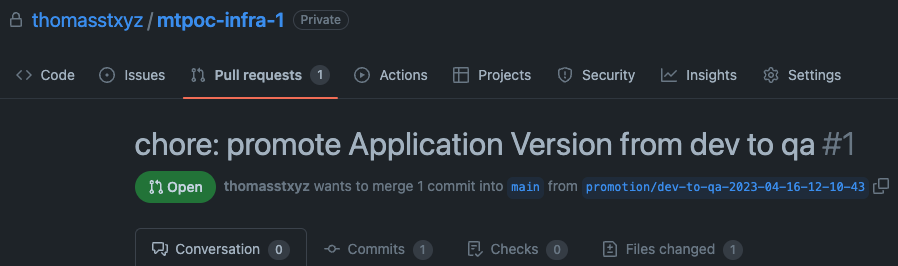
\includegraphics[width=1.00\linewidth]{assets/new-promotion-github.png}
%	\caption{New Git Pull Request.
%		%		(\citeauthor{ref}, \citeyear{ref}).
%	}
%	\label{fig:new-promotion-github}	
%\end{figure}
\begin{figure}[h]
	\centering
	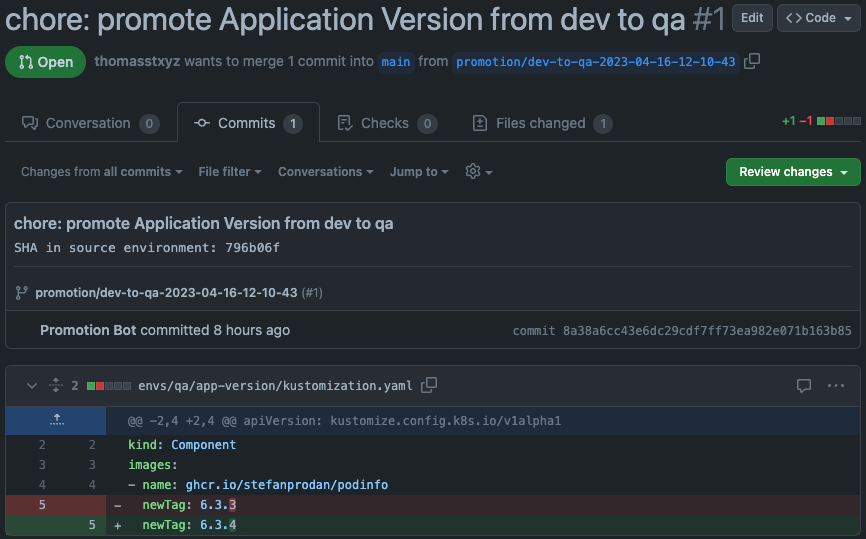
\includegraphics[width=1.00\linewidth]{assets/prom-pr-dev-to-qa.png}
	\caption{Pull Request for Promotion from dev to qa.
		%		(\citeauthor{ref}, \citeyear{ref}).
	}
	\label{fig:prom-pr-dev-to-qa}	
\end{figure}

The changed difference introduced by the commit can be viewed:

\begin{lstlisting}
- newTag: 6.3.3
+ newTag: 6.3.4
\end{lstlisting}

The \lstinline|dev-to-qa| promotion requested the change of the image version from
\lstinline|6.3.3| to \lstinline|6.3.4|.

Now, since the \lstinline|qa| and the \lstinline|prod-1| environments
also differ,
a pull request has also been created for this promotion.

%\begin{figure}[h]
%	\centering
%	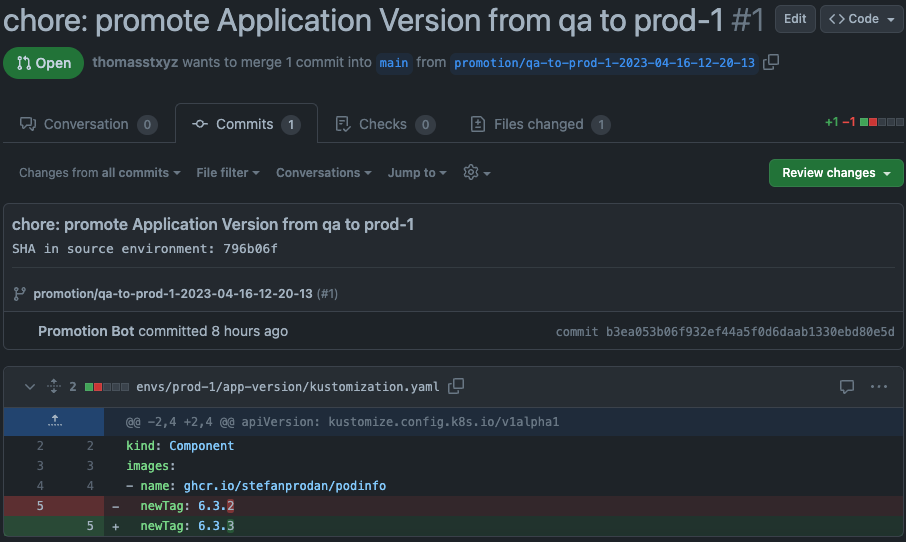
\includegraphics[width=1.00\linewidth]{assets/prom-pr-qa-to-prod-1.png}
%	\caption{Pull Request for Promotion from qa to prod-1.
%		%		(\citeauthor{ref}, \citeyear{ref}).
%	}
%	\label{fig:prom-pr-qa-to-prod-1}	
%\end{figure}

The \lstinline|qa-to-prod-1| promotion requested the change of the image version from
\lstinline|6.3.2| to \lstinline|6.3.3|.

\begin{lstlisting}
- newTag: 6.3.2
+ newTag: 6.3.3
\end{lstlisting}

Now, since the \lstinline|prod-1| and the \lstinline|prod-2| environments
also differ,
a pull request has also been created for this promotion.

%\begin{figure}[h]
%	\centering
%	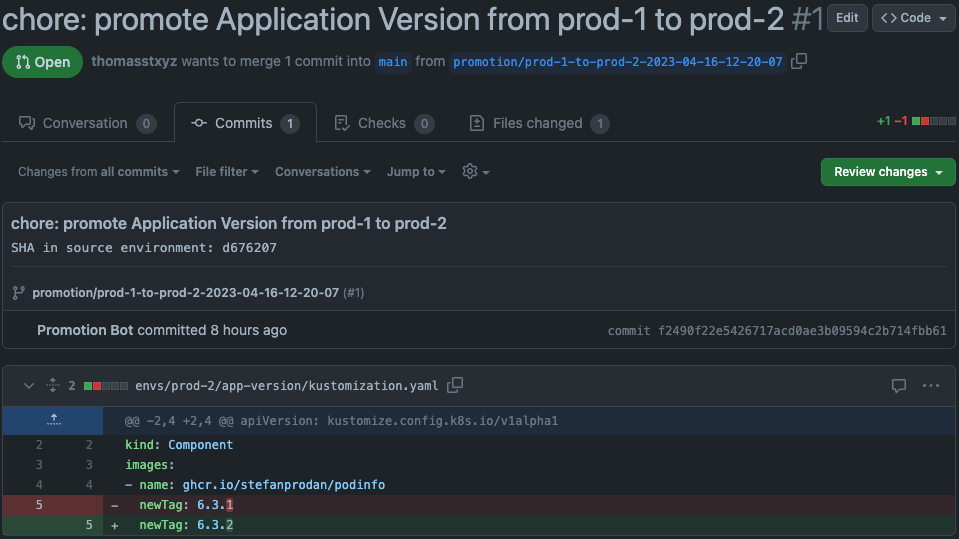
\includegraphics[width=1.00\linewidth]{assets/prom-pr-prod-1-to-prod-2.png}
%	\caption{Pull Request for Promotion from prod-1 to prod-2.
%		%		(\citeauthor{ref}, \citeyear{ref}).
%	}
%	\label{fig:prom-pr-prod-1-to-prod-2}	
%\end{figure}

The \lstinline|prod-1-to-prod-2| promotion requested the change of the image version from
\lstinline|6.3.1| to \lstinline|6.3.2|.

\begin{lstlisting}
- newTag: 6.3.1
+ newTag: 6.3.2
\end{lstlisting}

If the \lstinline|dev| environment advances the application image version further,
the pull request for the \lstinline|dev-to-qa| will be updated with another commit.
Note that the previous commit is not overwritten, 
but the commit history is kept on the pull request branch - now there are two commits on the branch.

\begin{figure}[h]
	\centering
	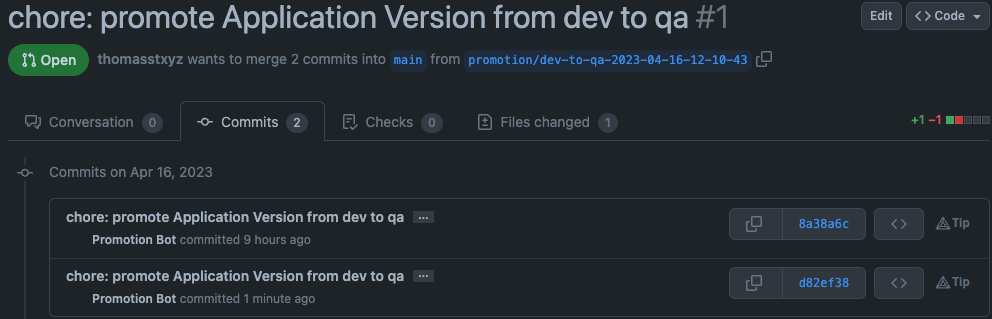
\includegraphics[width=1.00\linewidth]{assets/prom-pr-dev-to-qa-round2.png}
	\caption{Pull Request updated for Promotion from dev to qa.
		%		(\citeauthor{ref}, \citeyear{ref}).
	}
	\label{fig:prom-pr-dev-to-qa-round2}	
\end{figure}

The difference for the \lstinline|dev-to-qa| promotion is now:

\begin{lstlisting}
- newTag: 6.3.3
+ newTag: 6.3.5
\end{lstlisting}

%\begin{figure}[h]
%	\centering
%	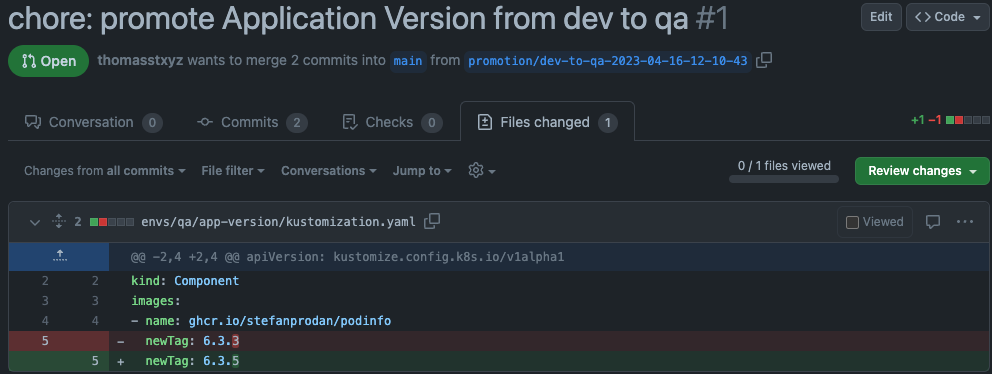
\includegraphics[width=1.00\linewidth]{assets/prom-pr-dev-to-qa-round2-diff.png}
%	\caption{Pull Request updated for Promotion from dev to qa (diff).
%		%		(\citeauthor{ref}, \citeyear{ref}).
%	}
%	\label{fig:prom-pr-dev-to-qa-round2-diff}	
%\end{figure}

Now if the pull request for the \lstinline|dev-to-qa| promotion
is approved and merged by a human,
the promotion will actually take effect.
This will results in the \lstinline|qa-to-prod-1| promotion pull request being updated
by the promotion controller.
Version \lstinline|6.3.5| is now requested for promotion to the
\lstinline|prod-1| environment.

The difference for the \lstinline|qa-to-prod-1| promotion is now:

\begin{lstlisting}
- newTag: 6.3.2
+ newTag: 6.3.5
\end{lstlisting}

Once reviewed, approved and merged by a human,
the promotion of version \lstinline|6.3.5| to the \lstinline|prod-1| environment
will result in further propagation of version \lstinline|6.3.5|
to the \lstinline|prod-2| environment.

The difference for the \lstinline|prod-1-to-prod-2| promotion pull request is now:

\begin{lstlisting}
- newTag: 6.3.1
+ newTag: 6.3.5
\end{lstlisting}

Once reviewed, approved and merged by a human,
the promotion of version \lstinline|6.3.5| to the \lstinline|prod-2| environment
will take effect.

The described demonstration showed,
how an application version can be promoted across multiple environments,
while ensuring a strict flow of promotion of \\
e.g. \lstinline|dev --> qa --> prod-1 --> prod-2|




%For this demonstration, it is supposed that
%the latest version \lstinline|6.3.5| is bad and should not be promoted,
%instead the \lstinline|dev| environment shall be rolled back to \lstinline|6.3.4|.






















\section{Evaluation Of Proof-of-Concept Use Cases}











\section{Summary}







%\chapter{Interviews with Working Professionals}
%
%\section{Categorisation of Findings}
%\section{Common Problem Definitions}
%\section{...?}
%
%
%\chapter{Definition of Solution Objectives}
%
%\section{People \& Communication Perspective}
%\section{Technical Perspective}
%\section{...?}
%
%
%\chapter{Prototype Design and Development}
%
%\section{Architecture}
%\section{Functionality}
%\section{...?}
%
%\chapter{Proof-of-Concept Demonstration}
%
%\section{Setup and Use with Kustomize}
%\section{Setup and Use with Helm}
%\section{Multiple Environments in same Stage}
%\section{Scalability}
%\section{...?}















%
%\section{Instruction included in the original FHBgld word processor template}
%Die Durchführung der empirischen Untersuchung ist nachvollziehbar zu dokumentieren sowie auch die dabei aufgetretenen Probleme und deren Behandlung. Der Umfang ergibt sich aus der Art der Bearbeitung.  
%
%Tabelle 1 zeigt ein Bespiel für eine Tabelle. 
%
%\begin{figure}[ht]
%	\centering
%	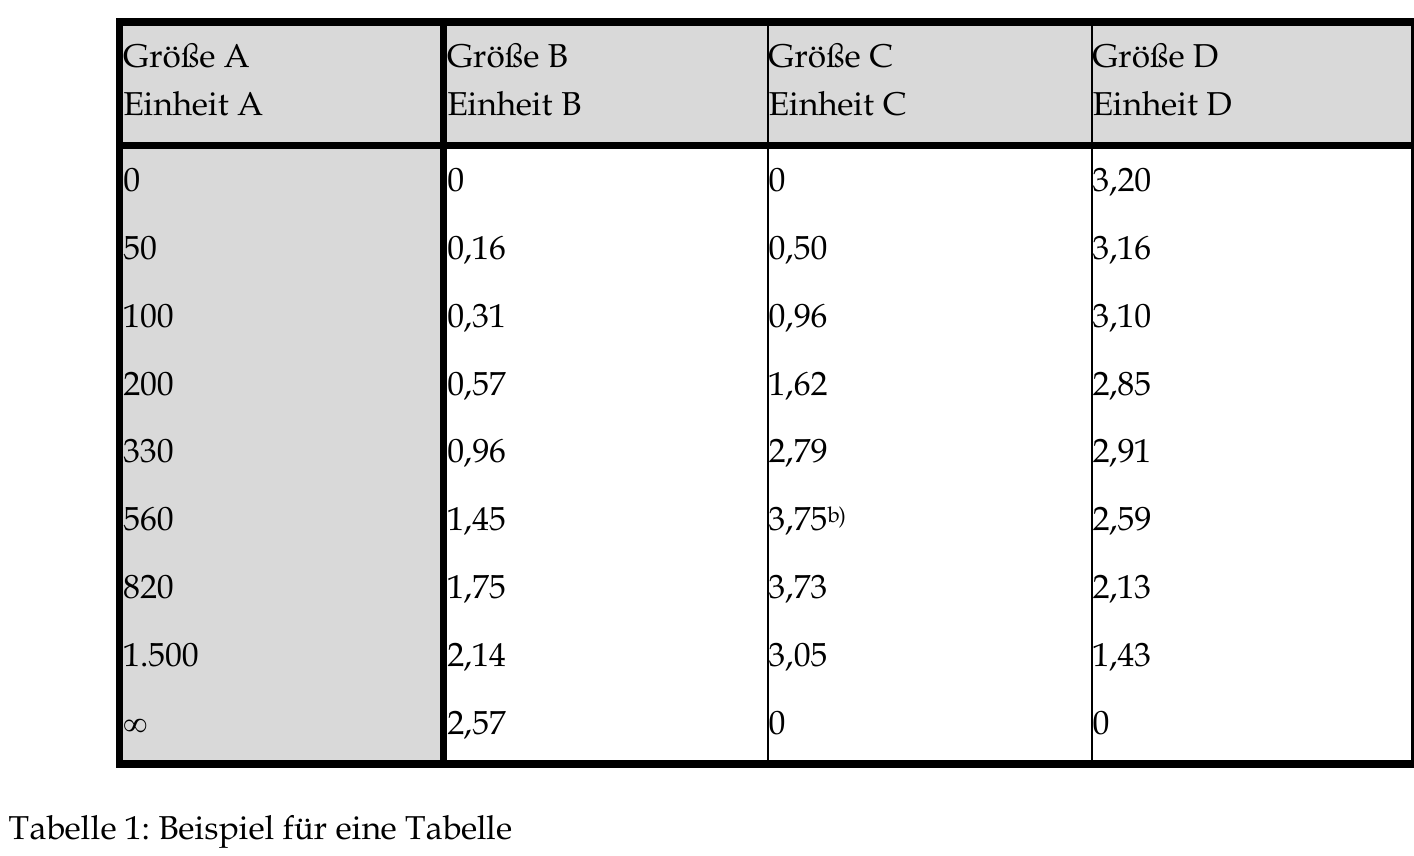
\includegraphics[width=0.7\linewidth]{figures/Word_Table}
%	\caption{Screenshot example from FHBgld word processor template}
%	\label{fig:wordtable}
%\end{figure}
%Abbildung 1 zeigt ein Beispiel für eine Abbildung oder Grafik.
%\begin{figure}
%	\centering
%	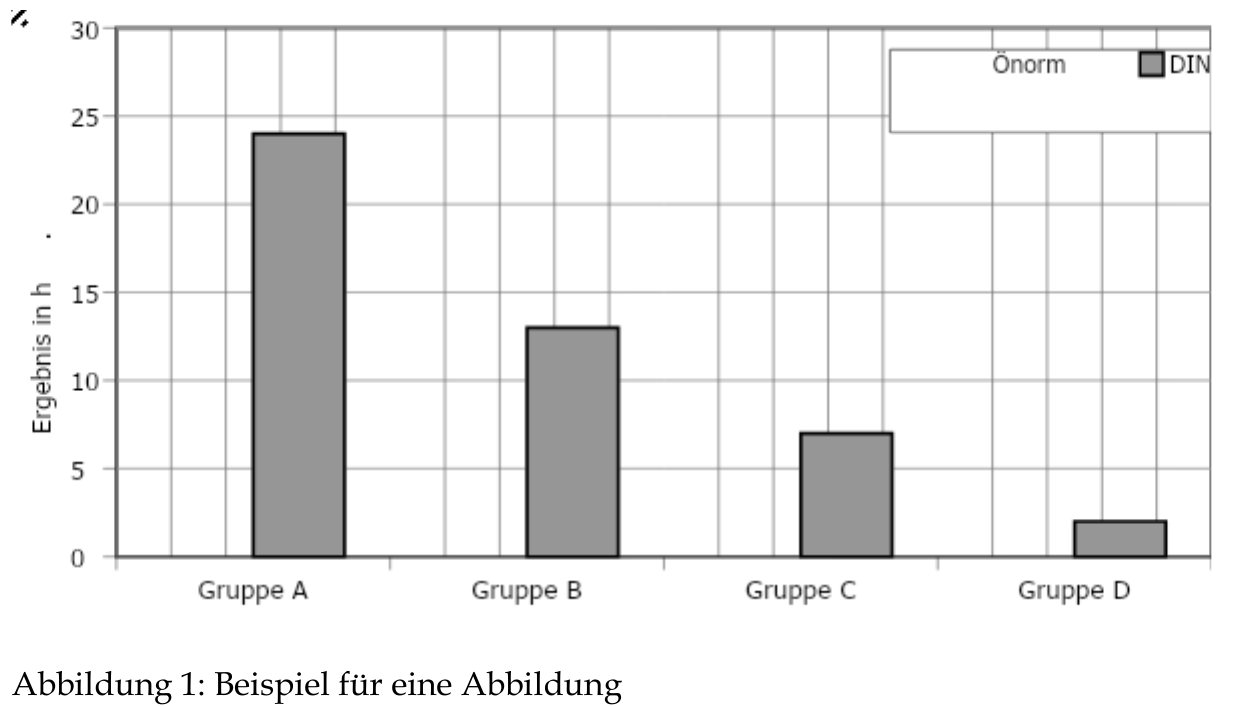
\includegraphics[width=0.7\linewidth]{figures/Word_Diagram}
%	\caption{Screenshot example from FHBgld word processor template}
%	\label{fig:worddiagram}
%\end{figure}
%\linebreak
%Mathematisch werden die Zusammenhänge wie im Figure \ref{fig:wordformel} beschrieben.
%\begin{figure}
%	\centering
%	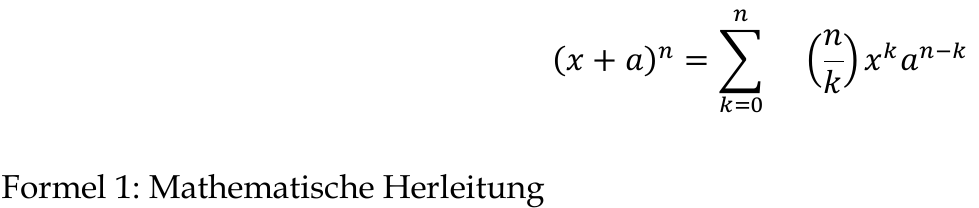
\includegraphics[width=0.7\linewidth]{figures/Word_Formel}
%	\caption{Screenshot example from FHBgld word processor template}
%	\label{fig:wordformel}
%\end{figure}
%
%\section{Tables and Images with \LaTeX}
%One of the great advantages of \LaTeX{} is that all it needs to know is
%the structure of a document, and then it will take care of the layout
%and presentation itself.  So, here we shall begin looking at how exactly
%you tell \LaTeX{} what it needs to know about your document.
%
%\subsection{Tables}
%In this sub-section, a simple table is inserted. To add reference to the table, see (cf. Table~\hyperref[tab:tableexample0]{\ref{tab:tableexample0}}):
%
%%A simple table.  The center environment is first set up, otherwise the
%%table is left aligned.  The tabular environment is what tells Latex
%%that the data within is data for the table.
%% https://en.wikibooks.org/wiki/LaTeX/Tables
%\begin{table}[htb]
%	\begin{tabular}{|b{7cm}|c|}
%		%The tabular environment is what tells Latex that the data within is
%		%data for the table.  The arguments say that there will be two
%		%columns, both left justified (indicated by the 'l', you could also
%		%have 'c' or 'r'.  The bars '|' indicate vertical lines throughout
%		%the table.
%		
%		\hline  % Print horizontal line
%		\fontsize{11pt}{12pt}\selectfont Command & Level \\ \hline  % Columns are delimited by '&'.  And
%		%rows are delimited by '\\'
%		\fontsize{10pt}{14pt}\selectfont Some sections to provide some examples: & \\
%		\texttt{\textbackslash part\{\emph{part}\}} & -1 \\
%		\texttt{\textbackslash chapter\{\emph{chapter}\}} & 0 \\
%		\texttt{\textbackslash section\{\emph{section}\}} & 1 \\
%		\texttt{\textbackslash subsection\{\emph{subsection}\}} & 2 \\
%		\texttt{\textbackslash subsubsection\{\emph{subsubsection}\}} & 3 \\
%		\texttt{\textbackslash paragraph\{\emph{paragraph}\}} & 4 \\
%		\texttt{\textbackslash subparagraph\{\emph{subparagraph}\}} & 5 \\
%		\hline
%		
%	\end{tabular}
%	\caption{some description of the table}
%	\label{tab:tableexample0}
%\end{table}
%
%\subsubsection{More tabular examples}
%
%First, a plain simple example for a FHBgld table, see table~\hyperref[tab:tab:tableexample1]{\ref{tab:tableexample1}}.
%
%\begin{table}[h]
%	\centering
%	\begin{tabular}{|b{1cm}|b{2cm}|b{3cm}|b{4cm}|}
%		\hline
%		\multicolumn{4}{|l|}{\fontsize{11pt}{12pt}\selectfont\noindent First line in 11pt fontsize } \\ \hline
%		1cm & 2cm & 3cm & 4cm \\ \hline
%		from & here on & the table & font size \\ \hline
%		will & be as & defined & in class, that is 10pt\footnote{yes, really!} \\ \hline
%		will & be as & defined & in class, that is 10pt\footnote{yes, really!} \\ \hline
%		will & be as & defined & in class, that is 10pt\footnote{yes, really!} \\ \hline
%		will & be as & defined & in class, that is 10pt\footnote{yes, really!} \\ \hline
%		will & be as & defined & in class, that is 10pt\footnote{yes, really!} \\ \hline
%	\end{tabular}
%	\caption{some description of the table}
%\label{tab:tableexample1}
%\end{table}
%
%Next, a table with nine columns, see table~\hyperref[tab:tableexample2]{\ref{tab:tableexample2}}.
%
%\begin{table}[h]
%	\centering
%	\begin{tabular}{|*{9}{l|}}
%		\hline
%		{\fontsize{11pt}{12pt}\selectfont This} & {\fontsize{11pt}{12pt}\selectfont table} & {\fontsize{11pt}{12pt}\selectfont has} & {\fontsize{11pt}{12pt}\selectfont way} & {\fontsize{11pt}{12pt}\selectfont too } & {\fontsize{11pt}{12pt}\selectfont many} & {\fontsize{11pt}{12pt}\selectfont columns}, & {\fontsize{11pt}{12pt}\selectfont does'nt} & {\fontsize{11pt}{12pt}\selectfont it?} \\ \hline
%		One & Two & Three & Four & Five & Six & Seven & Eight & Nine! \\ \hline
%		At & least & the & first & column & has & 11pt & font & size. \\ \hline
%	\end{tabular}
%	\caption{some description of the table}
%	\label{tab:tableexample2}
%\end{table}
%
%\subsection{Images}
%% Here is how to insert an image as a figure. There is a lot more you can do
%% when inserting images, check out: https://en.wikibooks.org/wiki/LaTeX/Importing_Graphics
%
%\begin{figure}[h]
%	\centering
%	
\includegraphics[width=0.3\textwidth]{figures/logo_nontransparent.jpg}
%	\caption{Image Example}
%	\label{fig:image_example}
%\end{figure}
%
%When an image is inserted, you can refer to it like this (cf. Figure~\hyperref[fig:image_example]{\ref{fig:image_example}}).
%
%\subsubsection{A Subsubsection}
%As one last example, this is how you can insert a sub-sub-section! Have fun
%writing your thesis with \LaTeX{}!
%
%\lipsum[2-3]
%\raggedbottom
%
%\pagebreak

%\chapter{Discussion and Interpretation}

%Results, Discussion and conclusions come here.

TODO

The overall goal of the thesis is to
provide a solution to the problem of release promotion in GitOps environments.
In this regard a prototype will be developed
and its functionality demonstrated in a proof-of-concept evaluation.
The goal for the prototype is to implement it as a modular extension to Kubernetes
and existing GitOps tooling.
By doing so, users can promote releases between multiple deployment environments
following the GitOps principles.
The main contribution of this thesis is a proof of concept for the developed prototype
which can be used as an extension to the GitOps toolkit within the CNCF.









\section{Learnings From The Prototype Implementation}

TODO

- ...

- User Feedback From Interview Partners








\section{Towards Standardized GitOps Promotions}

TODO






\section{Related Ideas And Approaches}

TODO






\section{?}
































%
%\section{Instruction included in the original FHBgld word processor template}
%Die Ergebnisse der Arbeit sind in übersichtlicher Form darzustellen Die gewählte Form der Darstellung ist vom gewählten Datenmaterial und den in der Einleitung gesetzten Zielen abhängig. Die Ergebnisse sind zu interpretieren und in Bezug zum Stand des Wissens zu diskutieren. Über die Beantwortung der Forschungsfrage und die daraus gezogenen Schlussfolgerungen schließt sich der Bogen zur Einleitung. 
%
%Wichtig ist die gedanklich klare Unterscheidung zwischen der Darstellung der Ergebnisse und der Interpretation/Bewertung der Ergebnisse. 
%
%\section{Code}
%If you want to show program code within your thesis you can use the \verb|\texttt{verbatim}| environment or for a more complex display take a look at \url{https://www.overleaf.com/learn/latex/Code_listing}
%
%\begin{verbatim}
%	Text enclosed inside \texttt{verbatim} environment 
%	is printed directly 
%	and all \LaTeX{} commands are ignored.
%\end{verbatim}
%
%\begin{lstlisting}[language=Python, caption=Python example]
%	import numpy as np
%	
%	def incmatrix(genl1,genl2):
%	m = len(genl1)
%	n = len(genl2)
%	M = None #to become the incidence matrix
%	VT = np.zeros((n*m,1), int)  #dummy variable
%	
%	#compute the bitwise xor matrix
%	M1 = bitxormatrix(genl1)
%	M2 = np.triu(bitxormatrix(genl2),1) 
%	
%	for i in range(m-1):
%	for j in range(i+1, m):
%	[r,c] = np.where(M2 == M1[i,j])
%	for k in range(len(r)):
%	VT[(i)*n + r[k]] = 1;
%	VT[(i)*n + c[k]] = 1;
%	VT[(j)*n + r[k]] = 1;
%	VT[(j)*n + c[k]] = 1;
%	
%	if M is None:
%	M = np.copy(VT)
%	else:
%	M = np.concatenate((M, VT), 1)
%	
%	VT = np.zeros((n*m,1), int)
%	
%	return M
%\end{lstlisting}

%\chapter{Future Work}
\label{future-work}

In this chapter,
further suggestions for future research on this topic and the developed prototype are presented.

In addition,
some interesting ideas that came out of this research are discussed,
and how they could be further researched in future work either by the researcher of this thesis or other researchers.



\section*{Further Research \& Development of the Prototype}

The proposed software prototype should be evaluated against its user experience,
in order to find out if users have difficulty doing the initial setup,
or any other troubles.
The use of the prototype could be observed in a case study or tested in a field experiment.
The prototype should be adapted in more iterations of the applied methodology process model.

The API, the custom resources, which the operator provides can be changed to fit the users needs.
Additional functionality which is required by users, can be added.
Since the operator works with any other GitOps tooling the users bring from their individual GitOps setup,
it can lack a bit of ease of use. The integration into other GitOps tooling like Argo or Flux
should be evaluated, and examined if such an integration is worth it, in order to provide better convenience.

The main goal is to extensively adapt for user requirements, in order to fit
many possible promotion processes.
The prototype should be further developed to enable the use in production by organizations or other projects.

\section*{Rolling Production Environments}

The term rolling production environments was coined by interview partner 1 during the interview.
It was discussed in section \ref{insights-related-ideas-approaches} earlier in this thesis.
The term represents a future idea of where promotions and rollouts of new releases could be heading to.
This approach steers in a somewhat other direction, than what this thesis researched.
Instead of having fixed testing environments or stages, which a new release needs to pass,
before being rolled out to the production environment,
this approach conversely foresees only the single environment,
which is actually used for production.

This approach builds upon the progressive delivery pattern,
which can be implemented with tools like Flagger or Argo Rollouts.
Instead of just doing progressive delivery of an application (i.e. Kubernetes deployment / container image),
the progressive delivery would be done on a whole environment (i.e. Kubernetes cluster).
This has the advantage of further limiting the chance of supporting services and applications
influencing the actual user-facing application in a bad way, i.e. breaking the service, making it unavailable for its users.
Each different supporting application constantly changes versions, and all these changes could potentially break some other dependency.
Some infrastructure components are sometimes even updated without a version history,
eliminating the possibility to roll back to a safe and working state.

One possible future work that could be done for evaluating this new approach,
could be to evaluate the costs and feasibility of this approach.
According to interview partner 1, tools like the Weave GitOps Terraform Controller
have made it a lot easier to achieve the idea of rolling production environments.
However since a whole production environment would be dynamically created with each new release,
this could introduce higher costs.
Especially in a cloud environment, where billing is done on-demand per minute used,
and where the costs can be an important factor for deciding between different architectures.

\section*{Overview of GitOps Repositories}

Discussed by interview partner 2 and presented in section \ref{insights-related-ideas-approaches}
is the idea and problem, that when a human is given a GitOps repository,
it is often difficult to understand how the setup is exactly structured,
what the environments are,
what the versions are,
and what applications and version are deployed where.
The overview that GitOps shall give,
with the single place to look and know what is your system's state,
is not as good as it is expected,
interview partner 2 mentioned.

As possible future research on this idea,
this problem statement could be evaluated with a survey research against GitOps users.
In addition, especially if the survey's results speak for this statement,
a software tool could be developed,
which can recognize filesystem structures and plain text configuration files,
which represent the desired state.
This tool would have have knowledge of the different configuration management tools like Kustomize or Helm.
It would probably be beneficial to have a visual representation in the form of a dashboard.

Such a visual representation is already provided by ArgoCD for example,
however it will only show the configured data in the dashboard.
Any files, which are not yet added to the specific ArgoCD instance,
can only be viewed by having a look into the Git repository's filesystem manually.




\section*{Towards Standardized GitOps Promotions}

There is no standard way of doing promotions with the GitOps approach.
Sometimes a container image tag is changed in some place or places,
other times multiple files are copied over to another place (like the promotion process proposed with the prototype in this thesis),
and other times a promotion consists of multiple processes spanning over different domains.
This differs for each individual setup for distinctive organizations.

In order to get a better understanding of what the requirements are for different organizations,
and how they imagine a solution, and solved their individual use case,
it would be of use to survey a wide range and variety of organizations which adopted or want to adopt the GitOps approach.
For open-source tooling it is beneficial to strive for functionality that can be used by everyone,
instead of providing tailored tooling which may only work for a single setup at a particular organization.

















\chapter{Conclusion}
\label{conclusion}

%In einer Conclusio wird keine neue Information präsentiert, sondern das bereits gesagte nochmal zusammenfassend wiedergegeben. Du möchtest hier dem Leser die wichtigsten Key Points deiner Arbeit mitgeben, so dass er sich ewig dran erinnernt.
%
%In welchem Forschungsfeld sind wir nochmal und was ist das eigentlich Problem dort?
%
%Welcher Lösungsvorschlag wurde präsentiert, um dieses Problem zu lösen und welche Methodik wird eingesetzt, um das zu schaffen?
%
%Ausblick...wenn wir das dann geschafft haben, was können wir dann mehr, was wir heute nicht können?
%
%Future Work -> welche neuen Forschungsfelder eröffnen sich dann, wo können wir ab dann weitermachen?


In this final chapter,
no new information is presented,
but what has already been said is summarized again.
The most important key points of the thesis are highlighted,
in order for the reader to easily consume.

\section*{Problem}

The increasing adoption of a DevOps culture in organizations to develop applications and services quickly,
and reduce friction between people, communications and technical processes,
to ultimately decrease the time to market for new product releases,
has brought forward a new practice called GitOps.

One of the unresolved problems of the GitOps practice is
the process of promoting releases between multiple deployment environments.
Current tools in the ecosystem do not provide an integrated solution for this process.
Users are therefore inclined to build workflows which are constrained to specific
Git providers, GitOps engines,
CI/CD system, and configuration/templating tools. This can lead to tightly coupled setups,
and vendor lock-in.

In this research,
the given problem was addressed by designing uniform, standardised models for
defining GitOps-native deployment environments and promotion processes.
These models were implemented in a prototype as custom resources and controllers with the
operator pattern, as a Kubernetes extension.
This developed software artifact allows users to define abstract representations
of their environments, and how they want releases to be promoted between them.

\section*{Research Question}

The overall goal of the thesis was to provide a solution to the problem of
release promotion in GitOps environments.
Therefore this overarching research question was defined:
\textbf{\ref{RQ1}};
with the following sub research questions:
\textbf{\ref{RQ1.1}}
\textbf{\ref{RQ1.2}}

\section*{Methodology}

In order to help with recognition and legitimization of the conducted research,
the methodology for conducting design science research in information systems
\autocite{designScienceResearchMethodologyForInformationSystemsResearch}
was applied, which consists of six activities.
%\nameref{methodology:activity1},
%\nameref{methodology:activity2},
%\nameref{methodology:activity3},
%\nameref{methodology:activity4},
%\nameref{methodology:activity5},
%\nameref{methodology:activity6}.
In activity 1,
the research problem of
release promotion with GitOps
was defined.
This was done primarily with the help of practicing professionals in the GitOps field,
which were interviewed.
In activity 2,
research objectives were inferred from the problem definition in activity 1.
Each objective maps to a distinct item from the problem specification,
which helped with later evaluation in activity 5.
In activity 3,
solutions for the previously defined objectives were designed and developed
by means of producing an artifact, namely the GitOps Promotions Operator prototype.
In activity 4,
the in-context use of the artifact was demonstrated in a proof of concept.
In activity 5,
the implementation of the artifact,
and how well it supports a solution to the problem,
was evaluated.
In activity 6, as a final step,
the whole conducted research was communicated by means of
publishing it as a master thesis.

\section*{Related Work}

Prior research on the concrete problem is focused on presenting
best practices and suggestions
which users need to manually implement themselves.
In addition it is suggested to let an external CI/CD system handle the promotion process.
Conversely, this thesis brought forward
abstract models of environments and promotion processes,
which are implemented in the proposed prototype operator,
as Kubernetes custom resources and controllers, with the operator framework.
The prototype will assess the feasibility of
defining deployment environments and promotion processes declaratively,
following the GitOps principles.

\section*{Theoretical Background}

The theoretical background on the topic was brought forward to the user,
in order to aid comprehension of the material within the thesis.
General definitions of terms,
fundamentals of GitOps along related tooling and components were presented.
DevOps and internal developer platforms were mentioned.
It was explained, how many times the term GitOps is misunderstood,
and that GitOps is actually defined in the OpenGitOps project.
It was shown how GitOps changes the architecture and process of Continuous Deployment,
and how the promotion of releases is achieved without and with the GitOps approach.
Emerging patterns like progressive delivery,
as well as the concept behind short-living environments were described.
The power of Kubernetes as a cloud native platform and its use cases beyond container orchestration were presented.
Finally it was shown how the declarative representations of GitOps environments are typically modelled currently.

\section*{Interviews}

For the problem identification and motivation of the main topic of this thesis,
%namely the promotion of releases in GitOps environments,
interviews with practicing professionals, who are working in the GitOps field, were conducted.
Several problems were identified,
and defined along with their respective research objectives.
\textbf{\nameref{problem1}},
relates to a frequent issue with currently available tooling in the GitOps ecosystem. 
Often times solely container image version tags are the focus with current tools when promoting
new versions or releases.
%It was discussed, that this is insufficient for some use cases.
Because it is sometimes required to handle all sorts of resources, not just the version tag of a container image,
an according research objective was defined.
%Especially when not using containerization technologies for runtime, this is an important problem to handle.
%In order to be able to provide a solution to this problem with a comprehensible approach,
%a solution objective was inferred and its requirements defined.
\textbf{\nameref{objective1}},
defines a qualitative description of how the respective problem is supposed to be solved
by the developed artifact. The main idea is to offer the capability to promote arbitrary resources,
meaning any type of resource, instead of solely the container image version.
%The technical implementation in the proposed prototype foresees the functionality for
%promoting a list of filesystem paths inside the Git repository of the desired state to other environments.
%In addition these arbitrary resources should be able to be assigned a descriptive name,
%in order to identify the promotion subjects more easily.
\textbf{\nameref{problem2}},
states the fact, that it is not a straight-forward process of how the order of promotion
through multiple GitOps environments can be setup.
%When adhering to the principles of GitOps
%and sticking with the asynchronous deployment process (described in the
%\nameref{theoretical-background} chapter)
%there is no streamlined approach or tooling, that automates this, while still sticking to the asynchronous process.
\textbf{\nameref{objective2}},
defines the requirements for the proposed prototype,
in regards to the according problem of having a certain order of promotion through environments or stages.
The objective describes the capability for defining a certain order of environments, in which releases traverse through.
In addition, this solution objective opens up the possibility to setup promotion in stages, in which
certain environments must be deployed to first, before the release can deploy to other specified environments.
\textbf{\nameref{problem3}},
relates to the problem that when wanting to promote a new release from environment one to another environment,
it is not easily achievable with the available tools to specify certain dependencies, like other workloads or
microservices in the same or another environment, or altogether dependencies from external sources.
This is especially desirable for evaluating test results or other metrics, before triggering the promotion.
\textbf{\nameref{objective3}},
describes how the respective problem of being able to specify dependencies for a promotion,
could be solved in the proposed prototype. While the minimum dependency is the successful deployment
of the workload of a release,
it may also be desirable to specify other resources or workloads which need to be in a certain state,
before triggering a promotion.
\textbf{\nameref{problem4}},
draws attention to the common problem of being dependent on single tools and providers.
The more complex the Continuous Delivery is setup for a particular project,
the more difficult it is to de-couple or switch providers for certain components.
%Furthermore, since many tools in the GitOps ecosystem are not very mature in their development and adoption,
%it is of use that components are loosely coupled and can be exchanged with alternatives in the future.
\textbf{\nameref{objective4}},
defines the requirements of how a vendor-neutral and tool-agnostic prototype can be implemented.
%The main components which are desirable to support all alternatives,
%for being able to switch between them,
%are the Git providers (e.g. GitHub, GitLab),
%the GitOps engines (e.g. Argo, Flux),
%the configuration/templating tools (e.g. Kustomize, Helm).
Additionally,
related ideas and approaches were discussed by the interview partners.
These points were not directly considered for the conducted design science in the prototype,
however they were discussed later.

\section*{Prototype}

The proposed prototype was presented.
The asynchronous nature of GitOps deployments, and where
the operator prototype fits within this architecture was described.
Abstract models for the environment and promotion custom resources as well as their prototype
design as declarative Kubernetes custom resources was described.
The implementation of these custom resources was shown in the form of mockups
of Kubernetes custom resources in the YAML format.
Alternative mockup designs were shown as a way to draw attention to the fact
that the actual design of the API specification is not cast in stone.
Moreover, the API specification should be tested with users of it,
and should be adapted for usability and ease of use.
The translation of the API specification in YAML format into Go types was described,
and finally the implemented controller logic of both the environment, as well as
the promotion controller was presented.
The developed artifact of the prototype operator was
demonstrated in the context of a proof-of-concept use case.
The demonstration of the prototype's functionality was then evaluated against
%the research objectives defined in
%\ref{interviews:definitionSolutionObjectives} \nameref{interviews:definitionSolutionObjectives}.
the research objectives.

\section*{Evaluation \& Results}

The results of the conducted research were presented, primarily by means of
presenting and describing the designed and developed operator prototype, and the learning
from the prototyping process.
In addition, the interviewed working professionals gave several interesting insights into the problem
statement from their point of view.
The results of the research were evaluated on how they provide a solution to the research problem.
The implemented functionality of the prototype was evaluated against the research objectives.
This was done by comparing the qualitative descriptions of the objectives with the actual observed results
in the demonstration of the prototype in the proof of concept.
% ?? feedback for the prototype from the working professionals??
For the research question RQ 1.1,
a possible solution was presented by means of
describing the design of a prototype of a Kubernetes operator for handling GitOps promotions.
For research question RQ 1.2,
a possible implementation of the abstract models was presented, in the form of
declarative custom resources, which extend the Kubernetes API.
The overarching research question 1 is the combination of the sub research questions.
The thesis proposes one possible way of how the research problem can be addressed,
namely the promotion of releases in GitOps environments can be designed.
This concrete research does not try to propose a definitive answer or solution to the research question.

\section*{Discussion \& Interpretation}

The results, learnings, and evaluations of the research were discussed and interpreted.
The meanings behind the specific results are brought forward in more detail.
Moreover, interpretations and implications of the results and evaluations were presented.
Learnings from implementing the prototype were presented, namely
ideas about the user experience, security considerations, the use at scale, abstractions and modularity.
Alternative approaches for promoting releases were presented, as mentioned by interview partner 1.
%
%The main idea of this approach is that long-living environments are not necessary,
%and the resiliency should rather be created by doing progressive delivery,
%not just for the user-facing application or service,
%but for the whole infrastructure stack below.
%This has the purpose of further increasing the immutability and resiliency of a service.
%Since the amount of supporting and infrastructure services and dependencies are increasing with Kubernetes,
%and each having a version and constantly new releases, and the possibility of breaking the actual important
%service that is user-facing.
%
%When following this approach, the end goal is to create a complete copy of the production environment,
%and then do progressive delivery on that.
%Once the release is marked as good, the old production environment can safely be destroyed.
%With the GitOps pattern, and the application and infrastructure being stored in Git,
%this has become increasingly more possible.
%Also tools like the Weave GitOps Terraform Controller have contributed to the enablement of this new approach. 
%
%While, with this approach, the need for long-living environments decreases,
%whole copies of production environments will still need to be created.
%This means there is no guarantee that the cost will decrease.
%Advanced tactics like auto-scaling will need to be implemented, in order to
%keep costs low of potentially high numbers of dynamically created environments.
%

\section*{Future Work}

Further suggestions and point of references for future research on this topic
and the developed prototype were presented.
These included
further research and development of the proposed prototype,
which is about testing its user experience, evaluating integration with
other GitOps tools. Generally the aim is to enhance the prototype
to make it mature for production use.
The idea of rolling production environments by interview partner 1 was discussed.
It describes a somewhat different approach for promotions in GitOps,
where less environments are needed, but for each new release the 
production environment is re-created with the new versions, and
progressive delivery is done not only on an application level, but on the whole
infrastructure stack together with the end user application or service on top.
This is to further improve immutability and versioning to increase resiliency.
The idea of the problem with the overview of GitOps repositories by interview partner 2
was discussed.
It is about the somewhat missing feature of an quick and easy to understand overview over a GitOps repository.
Depending on the used configuration/templating tool, a setup looks different.
Deployment environments can be represented, however it is not possible for the user
to know what the target environment is, or where the GitOps definition is deployed to in general.
Moreover it was discussed that it would make sense for future work
to research a wide range and variety of organizations and do a survey on
their requirements, their issues and how they imagine a solution.
An initiative towards standardized GitOps promotions should be made,
because for open-source tooling the aim should be to strive for functionality
that can be used by everyone,
instead of providing tailored tooling which may only be beneficial for specific use cases
and organizations.



























%The currently available GitOps tools
%do not provide an integrated solution to
%the problem of promoting releases between environments.
%This thesis aims at addressing the given problem.
%This is achieved by
%clearly defining the problem in distinct items,
%from which research objectives are then inferred.
%Following in designing and developing abstract models for
%environments and promotion processes;
%which are implemented in the produced artifact "release promotion operator".
%The artifact is demonstrated in a prototype serving as a proof-of-concept.
%Finally the research is evaluated by means of
%comparing the artifact's functionality with the solution objectives.
%
%The developed "release promotion operator" prototype should serve as
%a modular extension to Kubernetes and existing GitOps tooling within the CNCF.
%It should provide a more streamlined and GitOps-native approach
%to the process of release promotion.
%For subsequent research projects the use of the prototype could
%be observed in a case study or tested in a field experiment,
%and adapted in another iteration of the applied methodology process model.
%The main goal for future work is the extensive adaption of the prototype
%to enable use in production by organizations or other projects.






























%
%\section{Instruction included in the original FHBgld word processor template}
%Die Zusammenfassung stellt die gesamte Arbeit – von der Einleitung bis zu den Ergebnissen - in Kurzform dar. Länge maximal 1,5 - 2 Seiten. 
%
%\section{Algorithms}
%
%If you want to show algorithms in your Thesis take a look at the \url{https://www.overleaf.com/learn/latex/algorithms} page. The \verb|algorithm2e| package is already included in the template. You can list algorithms in the same way as you can list Tables and Figures.
%
%\begin{algorithm}[H]
%	\KwData{this text}
%	\KwResult{how to write algorithm with \LaTeX2e }
%	initialization\;
%	\While{not at end of this document}{
%		read current\;
%		\eIf{understand}{
%			go to next section\;
%			current section becomes this one\;
%		}{
%			go back to the beginning of current section\;
%		}
%	}
%	\caption{How to write algorithms}
%\end{algorithm}
%%\cleardoublepage{}
%
%\section{Acronyms and Glossary.}
%
%if you want to use Acronyms or a Glossary check the page here: \url{https://www.overleaf.com/learn/latex/glossaries}
%
%The \Gls{latex} typesetting markup language is specially suitable 
%for documents that include \gls{maths}. are 
%rendered properly an easily once one gets used to the commands.
%
%Given a set of numbers, there are elementary methods to compute 
%its \glsxtrlong{gcd}, which is abbreviated \glsxtrshort{gcd}. This 
%process is similar to that used for the \glsxtrfull{lcm}.
%
%\section{Macros}
%
%You can also add useful packages or macros into the \verb|packages_macros.tex| file to add them to the project.
%The packages for algorithms, code or the glossary have already been added there.
%
%\subsection{FixMe}
%Another example, the \verb|FixMe| package, is added as well. It allows you or your supervisor to add Meta comments to the document. These comments only appear if you set the draft mode in the \verb|main.tex| file. If you remove or comment the activation of the draft mode you can see your final thesis without comments.
\chapter{Einleitung und Problemhintergrund}

Adaptives Scheduling von Arbeitslasten in heterogenen Cluster-Umgebungen, basierend auf Energieeffizienz

Forschungsfeld (Universum), 5-7 Sätze

Was ist denn das überhaupt

Idee 1

Idee 2

Idee 3

Idee xy

Zusammenfassung

Problemstellung, 5-7 Sätze

Forschungsvorhaben, 5-7 Sätze

Ausblick, 3-5 Sätze


\titleformat{\chapter}{\normalfont\Large}{\thechapter}{20pt}{\normalfont\Large}
\printbibliography[title=\thesisBookLiteratureLabel]
\end{document}

%\documentclass[toc=chapterentrywithdots,a4paper,fontsize=12pt,listof=totoc,bibliography=totoc]{scrbook}
\pagestyle{plain} % no running headers, but page number in footer as required by FHBgld
%--Packages added by Dominik Thiede
\usepackage[table,xcdraw]{xcolor} % Use colours in table
\usepackage{pifont} %Use Latex Symbols like check mark 
\newcommand{\cmark}{\ding{51}}
\newcommand{\xmark}{\ding{55}}
\newcommand{\omark}{\ding{72}}
\usepackage{listings} % line break for programm code
\usepackage{xcolor} % highlighting text
\usepackage{glossaries}
% -- Packages needed in the class
\usepackage{scrhack}
%\usepackage[a-1b]{pdfx} % Required for PDF-A compliance 
\usepackage[left=2.5cm,right=2.5cm,top=2.5cm,bottom=2cm,bindingoffset=1cm]{geometry} % required for exact FHBgld page margins
%if changed to \usepackage[ngerman]{babel} "Table of contents" changes to "Inhaltsverzeichnis", "abstract" becomes "Zusammenfassung" and "references" is translated to "Literatur".
\usepackage[ngerman, british]{babel} 
\usepackage{graphicx} % Required for including pictures
%\usepackage[pdfa]{hyperref} % Required for PDF-A compliance 
\usepackage[hidelinks,pdfpagelayout=TwoPageRight]{hyperref} % FHBgld - Hide links: border and color
%\usepackage[hidelinks]{hyperref}
\usepackage[T1]{fontenc} % Required for accented characters
%\usepackage[utf8]{inputenc} % legacy, not needed
\usepackage{changepage} % detects odd/even pages
\usepackage[final]{microtype}
\usepackage{xurl}
\usepackage{mathpazo} % FHBgld required "Book Antiqua" font is a clone of Palatino
% \usepackage[natbib=true, backend=biber, style=apa, sorting=nty]{biblatex} % FHBgld APA bibliography style
%\addbibresource{bibliography.bib} % Bibilography resource file % this goes into the main.tex, otherwise some editors wont find it
\setcounter{secnumdepth}{4} % FHBgld Numbering depth
%\setcounter{tocdepth}{3} % FHBgld TOC depth
\usepackage{csquotes} % Context sensitive quotation facilities, needed for babel and Biblatex-APA to work
\usepackage{booktabs} % Publication quality tables in LaTeX
\usepackage{tabularx} % Tabulars with adjustable-width columns.
\usepackage{multirow} % Create tabular cells spanning multiple rows
\usepackage{algorithm2e} % Package to show algorithms
\usepackage{listings} % Package to format code
\usepackage{xcolor} % Driver-independent color extensions for LaTeX
%\usepackage[super]{nth} % superscript
\usepackage{fmtcount} % another superscript ;-)
\usepackage{verbatim} % provides \begin{verbatim} formatting
\usepackage{array} % additional functionality for the tabular environment

\usepackage[record=only,acronym,nonumberlist,nopostdot=false,toc=true,style=super]{glossaries-extra} % provides extra glossaries features plus bib2gls, use convertgls2bib  defns.tex defns.bib to convert
\usepackage[justification=RaggedRight,singlelinecheck=false,font=footnotesize]{caption} % Needed to format captions to align left
%\RequirePackage{tocloft} % allows to change directories

% \usepackage{showframe}  % Draw a page-layout diagram on pages, RMF

\usepackage{lipsum} % lipsum :-) , RMF 

%  -- colors
\definecolor{codegreen}{rgb}{0,0.6,0}
\definecolor{codegray}{rgb}{0.5,0.5,0.5}
\definecolor{codepurple}{rgb}{0.58,0,0.82}
\definecolor{backcolour}{rgb}{0.95,0.95,0.92}

%  -- FHBgld fonts
% regular fontsize=12pt set in scrbook and mathpazo for Palatino-Roman above
\setkomafont{disposition}{\bfseries} % bold+fat for all sectioning command titles
\addtokomafont{title}{\fontsize{24}{24}\selectfont} % FHBgld Title
\addtokomafont{subtitle}{\fontsize{14}{16}\selectfont} % FHBgld Subtitle
%\addtokomafont{part}{\fontsize{16}{16}\selectfont} % FHBgld Level 1
\addtokomafont{chapter}{\fontsize{16}{16}\selectfont} % FHBgld Level 1
\addtokomafont{section}{\fontsize{14}{16}\selectfont} % FHBgld Level 2
\addtokomafont{subsection}{\fontsize{14}{16}\selectfont} % FHBgld Level 3
\addtokomafont{subsubsection}{\fontsize{13}{16}\selectfont} % FHBgld Level 4

% -- Default table fontsize according to FHBgld requirements
\let\oldtabular\tabular 
\renewcommand{\tabular}{\fontsize{10pt}{14pt}\selectfont\oldtabular}
% FHBgld wants the first line to have 11pt, unfortunately the array package lets you configure columns only. 
% Therefore, each cell of the first line of a table is formatted as follows:
% {\fontsize{11pt}{12pt}\selectfont <content here> }

%  -- FHBgld paragraphs etc.
\setlength{\parskip}{6pt} % Paragraph distance 6pt as required by FHBgld
\setlength\parindent{0pt} % No indent as required by FHBgld
\setlength{\footskip}{2.5\baselineskip} % Move Textbody close to footer as required by FHBgld
\renewcommand*{\chapterheadstartvskip}{\vspace*{0cm}} % FHBgld starts chapter aligned to top


\RedeclareSectionCommand[beforeskip=0pt,afterskip=.5\baselineskip plus .1\baselineskip minus .167\baselineskip]{chapter}
\RedeclareSectionCommand[beforeskip=-1\baselineskip,afterskip=.2\baselineskip]{section}
\RedeclareSectionCommand[beforeskip=-.75\baselineskip,afterskip=.5\baselineskip]{subsection}
\RedeclareSectionCommand[beforeskip=-.75\baselineskip,afterskip=.25\baselineskip]{subsubsection}
\RedeclareSectionCommand[beforeskip=.5\baselineskip,afterskip=-1em]{paragraph}
\RedeclareSectionCommand[beforeskip=-.5\baselineskip,afterskip=-1em]{subparagraph}

% %\renewcommand{\rmdefault}{pplj} % Replaces all Roman fonts with pplj (Palatino-Roman) if \usepackage{palatino}, not mathpazo

% TODO: also move to  thesis-book preamble
\hyphenation{GitOps}
\hyphenation{OpenGitOps}
\hyphenation{Kubernetes}
\hyphenation{Kustomize}

\makeatletter
\newcommand{\setword}[2]{%
  \phantomsection
  #1\def\@currentlabel{\unexpanded{#1}}\label{#2}%
}
\makeatother



\renewcommand{\autodot}{}% Remove all end-of-counter dots


% %%%%%%%%%%%%%%%%%%%%additional packages and macros%%%%%%%%%%%%%%%%%%%%%%%%%%%%%%
%\usepackage{algorithm2e}
%\usepackage[acronym]{glossaries}
%packages and setings to show colored code
%\usepackage{listings}
%\usepackage{xcolor}
%\definecolor{codegreen}{rgb}{0,0.6,0}
%\definecolor{codegray}{rgb}{0.5,0.5,0.5}
%\definecolor{codepurple}{rgb}{0.58,0,0.82}
%\definecolor{backcolour}{rgb}{0.95,0.95,0.92}

\lstdefinestyle{mystyle}{
    backgroundcolor=\color{backcolour},   
    commentstyle=\color{codegreen},
    keywordstyle=\color{magenta},
    numberstyle=\tiny\color{codegray},
    stringstyle=\color{codepurple},
    basicstyle=\ttfamily\footnotesize,
    breakatwhitespace=false,         
    breaklines=true,                 
    captionpos=b,                    
    keepspaces=true,                 
    numbers=left,                    
    numbersep=5pt,                  
    showspaces=false,                
    showstringspaces=false,
    showtabs=false,                  
    tabsize=2
}

\lstset{style=mystyle}

%\usepackage{showframe}


%%%%%%%%%%%%%%%%%%% added to thesis draft %%%%%%%%%%%%%%%%%%%%%%%%%%%%%%%%
\usepackage{acro}
\usepackage[
    urldate=long,		    % default: short, e.g. 08/15/2010
    style=authoryear-icomp,	% Harvard citation style
    sorting=nty,            % this is default: sort by name, title, year
    style=apa,
    backend=biber,
    language=ngerman,
    sortlocale=de-DE,    % set according to your needs
    natbib=true,		    % if you want to use natbib compatible citation commands; do _not_ use package natbib!
    maxbibnames=1000,
]{biblatex}
\addbibresource{references.bib}


% add content to the files in B_Chapters

% more content needed?
% add additional chapter files to B_Chapters
% input the new files in thesis/thesis-book